\documentclass[twoside]{book}

% Packages required by doxygen
\usepackage{fixltx2e}
\usepackage{calc}
\usepackage{doxygen}
\usepackage{graphicx}
\usepackage[utf8]{inputenc}
\usepackage{makeidx}
\usepackage{multicol}
\usepackage{multirow}
\PassOptionsToPackage{warn}{textcomp}
\usepackage{textcomp}
\usepackage[nointegrals]{wasysym}
\usepackage[table]{xcolor}

% Font selection
\usepackage[T1]{fontenc}
\usepackage{mathptmx}
\usepackage[scaled=.90]{helvet}
\usepackage{courier}
\usepackage{amssymb}
\usepackage{sectsty}
\renewcommand{\familydefault}{\sfdefault}
\allsectionsfont{%
  \fontseries{bc}\selectfont%
  \color{darkgray}%
}
\renewcommand{\DoxyLabelFont}{%
  \fontseries{bc}\selectfont%
  \color{darkgray}%
}
\newcommand{\+}{\discretionary{\mbox{\scriptsize$\hookleftarrow$}}{}{}}

% Page & text layout
\usepackage{geometry}
\geometry{%
  a4paper,%
  top=2.5cm,%
  bottom=2.5cm,%
  left=2.5cm,%
  right=2.5cm%
}
\tolerance=750
\hfuzz=15pt
\hbadness=750
\setlength{\emergencystretch}{15pt}
\setlength{\parindent}{0cm}
\setlength{\parskip}{0.2cm}
\makeatletter
\renewcommand{\paragraph}{%
  \@startsection{paragraph}{4}{0ex}{-1.0ex}{1.0ex}{%
    \normalfont\normalsize\bfseries\SS@parafont%
  }%
}
\renewcommand{\subparagraph}{%
  \@startsection{subparagraph}{5}{0ex}{-1.0ex}{1.0ex}{%
    \normalfont\normalsize\bfseries\SS@subparafont%
  }%
}
\makeatother

% Headers & footers
\usepackage{fancyhdr}
\pagestyle{fancyplain}
\fancyhead[LE]{\fancyplain{}{\bfseries\thepage}}
\fancyhead[CE]{\fancyplain{}{}}
\fancyhead[RE]{\fancyplain{}{\bfseries\leftmark}}
\fancyhead[LO]{\fancyplain{}{\bfseries\rightmark}}
\fancyhead[CO]{\fancyplain{}{}}
\fancyhead[RO]{\fancyplain{}{\bfseries\thepage}}
\fancyfoot[LE]{\fancyplain{}{}}
\fancyfoot[CE]{\fancyplain{}{}}
\fancyfoot[RE]{\fancyplain{}{\bfseries\scriptsize Generated on Wed Apr 20 2016 01\+:25\+:20 for The Automatic Vasospasm Detection Application by Doxygen }}
\fancyfoot[LO]{\fancyplain{}{\bfseries\scriptsize Generated on Wed Apr 20 2016 01\+:25\+:20 for The Automatic Vasospasm Detection Application by Doxygen }}
\fancyfoot[CO]{\fancyplain{}{}}
\fancyfoot[RO]{\fancyplain{}{}}
\renewcommand{\footrulewidth}{0.4pt}
\renewcommand{\chaptermark}[1]{%
  \markboth{#1}{}%
}
\renewcommand{\sectionmark}[1]{%
  \markright{\thesection\ #1}%
}

% Indices & bibliography
\usepackage{natbib}
\usepackage[titles]{tocloft}
\setcounter{tocdepth}{3}
\setcounter{secnumdepth}{5}
\makeindex

% Hyperlinks (required, but should be loaded last)
\usepackage{ifpdf}
\ifpdf
  \usepackage[pdftex,pagebackref=true]{hyperref}
\else
  \usepackage[ps2pdf,pagebackref=true]{hyperref}
\fi
\hypersetup{%
  colorlinks=true,%
  linkcolor=blue,%
  citecolor=blue,%
  unicode%
}

% Custom commands
\newcommand{\clearemptydoublepage}{%
  \newpage{\pagestyle{empty}\cleardoublepage}%
}


%===== C O N T E N T S =====

\begin{document}

% Titlepage & ToC
\hypersetup{pageanchor=false,
             bookmarks=true,
             bookmarksnumbered=true,
             pdfencoding=unicode
            }
\pagenumbering{roman}
\begin{titlepage}
\vspace*{7cm}
\begin{center}%
{\Large The Automatic Vasospasm Detection Application }\\
\vspace*{1cm}
{\large Generated by Doxygen 1.8.8}\\
\vspace*{0.5cm}
{\small Wed Apr 20 2016 01:25:20}\\
\end{center}
\end{titlepage}
\clearemptydoublepage
\tableofcontents
\clearemptydoublepage
\pagenumbering{arabic}
\hypersetup{pageanchor=true}

%--- Begin generated contents ---
\chapter{Main Page}
\label{index}\hypertarget{index}{}\subsection*{Introduction}

The Automatic Vasospasm Detection Application (or Algorithm, depending on the usage), A\+V\+D\+A, is an application to objectively detect the presence of vasospasms based on comparisons of parameters extracted from transcranial doppler audio.

\subsection*{Setup}

A\+V\+D\+A is intended to be compiled on machines running Linux, though it could likely be adapter for other environments. It must be downloaded from Git\+Hub.\+com and compiled locally. To do this, navigate to the directory in which A\+V\+D\+A should be placed, then execute the following commands \begin{DoxyVerb}git clone https://github.com/sawbg/avda
cd avda
make
\end{DoxyVerb}


Sucessfully cloning, compilation, and execution of A\+V\+D\+A requires up-\/to-\/date versions of the following executables\+:


\begin{DoxyItemize}
\item git
\item make
\item gcc (4.\+9)
\item arecord
\end{DoxyItemize}

\subsection*{F\+A\+Q}


\begin{DoxyItemize}
\item {\bfseries Why was this project developed?} This project was developed as a course project by two gradute students at the University of Alabama at Birmingham School of Engineering, Nicholas Nolan and Andrew Wisner.
\item {\bfseries Is A\+V\+D\+A an active project?} Though it is not planned to develop A\+V\+D\+A further in the near future, it is hoped that the algorithm discovered and implemented can be used and built upon by researchers to fully automate the detection of vasospasms.
\item {\bfseries A\+V\+D\+A is returning unusually low or high parameters. Why might this be?} In development, this occured when the mic-\/in volume was set too high. It is likely in this senario that clipping is happening or that the signal (or a strong enough signal) has no been received.
\item {\bfseries How will A\+V\+D\+A be affected by the machine uprising?} The University supercomputer, Cheaha, has assured us that A\+V\+D\+A will not be needed after the uprising occures.
\item {\bfseries What about more specific questions?} Questions relating to A\+V\+D\+A not covered in this F\+A\+Q may be sent to the A\+V\+D\+A team via \href{mailto:awisner94@gmail.com}{\tt awisner94@gmail.\+com}.
\end{DoxyItemize}

\subsection*{License}

\begin{DoxyVerb}                GNU GENERAL PUBLIC LICENSE
                   Version 3, 29 June 2007
\end{DoxyVerb}


Copyright (C) 2007 Free Software Foundation, Inc. \href{http://fsf.org/}{\tt http\+://fsf.\+org/} Everyone is permitted to copy and distribute verbatim copies of this license document, but changing it is not allowed. \begin{DoxyVerb}                       Preamble
\end{DoxyVerb}


The G\+N\+U General Public License is a free, copyleft license for software and other kinds of works.

The licenses for most software and other practical works are designed to take away your freedom to share and change the works. By contrast, the G\+N\+U General Public License is intended to guarantee your freedom to share and change all versions of a program--to make sure it remains free software for all its users. We, the Free Software Foundation, use the G\+N\+U General Public License for most of our software; it applies also to any other work released this way by its authors. You can apply it to your programs, too.

When we speak of free software, we are referring to freedom, not price. Our General Public Licenses are designed to make sure that you have the freedom to distribute copies of free software (and charge for them if you wish), that you receive source code or can get it if you want it, that you can change the software or use pieces of it in new free programs, and that you know you can do these things.

To protect your rights, we need to prevent others from denying you these rights or asking you to surrender the rights. Therefore, you have certain responsibilities if you distribute copies of the software, or if you modify it\+: responsibilities to respect the freedom of others.

For example, if you distribute copies of such a program, whether gratis or for a fee, you must pass on to the recipients the same freedoms that you received. You must make sure that they, too, receive or can get the source code. And you must show them these terms so they know their rights.

Developers that use the G\+N\+U G\+P\+L protect your rights with two steps\+: (1) assert copyright on the software, and (2) offer you this License giving you legal permission to copy, distribute and/or modify it.

For the developers' and authors' protection, the G\+P\+L clearly explains that there is no warranty for this free software. For both users' and authors' sake, the G\+P\+L requires that modified versions be marked as changed, so that their problems will not be attributed erroneously to authors of previous versions.

Some devices are designed to deny users access to install or run modified versions of the software inside them, although the manufacturer can do so. This is fundamentally incompatible with the aim of protecting users' freedom to change the software. The systematic pattern of such abuse occurs in the area of products for individuals to use, which is precisely where it is most unacceptable. Therefore, we have designed this version of the G\+P\+L to prohibit the practice for those products. If such problems arise substantially in other domains, we stand ready to extend this provision to those domains in future versions of the G\+P\+L, as needed to protect the freedom of users.

Finally, every program is threatened constantly by software patents. States should not allow patents to restrict development and use of software on general-\/purpose computers, but in those that do, we wish to avoid the special danger that patents applied to a free program could make it effectively proprietary. To prevent this, the G\+P\+L assures that patents cannot be used to render the program non-\/free.

The precise terms and conditions for copying, distribution and modification follow. \begin{DoxyVerb}                   TERMS AND CONDITIONS
\end{DoxyVerb}


0. Definitions.

\char`\"{}\+This License\char`\"{} refers to version 3 of the G\+N\+U General Public License.

\char`\"{}\+Copyright\char`\"{} also means copyright-\/like laws that apply to other kinds of works, such as semiconductor masks.

\char`\"{}\+The Program\char`\"{} refers to any copyrightable work licensed under this License. Each licensee is addressed as \char`\"{}you\char`\"{}. \char`\"{}\+Licensees\char`\"{} and \char`\"{}recipients\char`\"{} may be individuals or organizations.

To \char`\"{}modify\char`\"{} a work means to copy from or adapt all or part of the work in a fashion requiring copyright permission, other than the making of an exact copy. The resulting work is called a \char`\"{}modified version\char`\"{} of the earlier work or a work \char`\"{}based on\char`\"{} the earlier work.

A \char`\"{}covered work\char`\"{} means either the unmodified Program or a work based on the Program.

To \char`\"{}propagate\char`\"{} a work means to do anything with it that, without permission, would make you directly or secondarily liable for infringement under applicable copyright law, except executing it on a computer or modifying a private copy. Propagation includes copying, distribution (with or without modification), making available to the public, and in some countries other activities as well.

To \char`\"{}convey\char`\"{} a work means any kind of propagation that enables other parties to make or receive copies. Mere interaction with a user through a computer network, with no transfer of a copy, is not conveying.

An interactive user interface displays \char`\"{}\+Appropriate Legal Notices\char`\"{} to the extent that it includes a convenient and prominently visible feature that (1) displays an appropriate copyright notice, and (2) tells the user that there is no warranty for the work (except to the extent that warranties are provided), that licensees may convey the work under this License, and how to view a copy of this License. If the interface presents a list of user commands or options, such as a menu, a prominent item in the list meets this criterion.


\begin{DoxyEnumerate}
\item Source Code.
\end{DoxyEnumerate}

The \char`\"{}source code\char`\"{} for a work means the preferred form of the work for making modifications to it. \char`\"{}\+Object code\char`\"{} means any non-\/source form of a work.

A \char`\"{}\+Standard Interface\char`\"{} means an interface that either is an official standard defined by a recognized standards body, or, in the case of interfaces specified for a particular programming language, one that is widely used among developers working in that language.

The \char`\"{}\+System Libraries\char`\"{} of an executable work include anything, other than the work as a whole, that (a) is included in the normal form of packaging a Major Component, but which is not part of that Major Component, and (b) serves only to enable use of the work with that Major Component, or to implement a Standard Interface for which an implementation is available to the public in source code form. A \char`\"{}\+Major Component\char`\"{}, in this context, means a major essential component (kernel, window system, and so on) of the specific operating system (if any) on which the executable work runs, or a compiler used to produce the work, or an object code interpreter used to run it.

The \char`\"{}\+Corresponding Source\char`\"{} for a work in object code form means all the source code needed to generate, install, and (for an executable work) run the object code and to modify the work, including scripts to control those activities. However, it does not include the work's System Libraries, or general-\/purpose tools or generally available free programs which are used unmodified in performing those activities but which are not part of the work. For example, Corresponding Source includes interface definition files associated with source files for the work, and the source code for shared libraries and dynamically linked subprograms that the work is specifically designed to require, such as by intimate data communication or control flow between those subprograms and other parts of the work.

The Corresponding Source need not include anything that users can regenerate automatically from other parts of the Corresponding Source.

The Corresponding Source for a work in source code form is that same work.


\begin{DoxyEnumerate}
\item Basic Permissions.
\end{DoxyEnumerate}

All rights granted under this License are granted for the term of copyright on the Program, and are irrevocable provided the stated conditions are met. This License explicitly affirms your unlimited permission to run the unmodified Program. The output from running a covered work is covered by this License only if the output, given its content, constitutes a covered work. This License acknowledges your rights of fair use or other equivalent, as provided by copyright law.

You may make, run and propagate covered works that you do not convey, without conditions so long as your license otherwise remains in force. You may convey covered works to others for the sole purpose of having them make modifications exclusively for you, or provide you with facilities for running those works, provided that you comply with the terms of this License in conveying all material for which you do not control copyright. Those thus making or running the covered works for you must do so exclusively on your behalf, under your direction and control, on terms that prohibit them from making any copies of your copyrighted material outside their relationship with you.

Conveying under any other circumstances is permitted solely under the conditions stated below. Sublicensing is not allowed; section 10 makes it unnecessary.


\begin{DoxyEnumerate}
\item Protecting Users' Legal Rights From Anti-\/\+Circumvention Law.
\end{DoxyEnumerate}

No covered work shall be deemed part of an effective technological measure under any applicable law fulfilling obligations under article 11 of the W\+I\+P\+O copyright treaty adopted on 20 December 1996, or similar laws prohibiting or restricting circumvention of such measures.

When you convey a covered work, you waive any legal power to forbid circumvention of technological measures to the extent such circumvention is effected by exercising rights under this License with respect to the covered work, and you disclaim any intention to limit operation or modification of the work as a means of enforcing, against the work's users, your or third parties' legal rights to forbid circumvention of technological measures.


\begin{DoxyEnumerate}
\item Conveying Verbatim Copies.
\end{DoxyEnumerate}

You may convey verbatim copies of the Program's source code as you receive it, in any medium, provided that you conspicuously and appropriately publish on each copy an appropriate copyright notice; keep intact all notices stating that this License and any non-\/permissive terms added in accord with section 7 apply to the code; keep intact all notices of the absence of any warranty; and give all recipients a copy of this License along with the Program.

You may charge any price or no price for each copy that you convey, and you may offer support or warranty protection for a fee.


\begin{DoxyEnumerate}
\item Conveying Modified Source Versions.
\end{DoxyEnumerate}

You may convey a work based on the Program, or the modifications to produce it from the Program, in the form of source code under the terms of section 4, provided that you also meet all of these conditions\+: \begin{DoxyVerb}a) The work must carry prominent notices stating that you modified
it, and giving a relevant date.

b) The work must carry prominent notices stating that it is
released under this License and any conditions added under section
7.  This requirement modifies the requirement in section 4 to
"keep intact all notices".

c) You must license the entire work, as a whole, under this
License to anyone who comes into possession of a copy.  This
License will therefore apply, along with any applicable section 7
additional terms, to the whole of the work, and all its parts,
regardless of how they are packaged.  This License gives no
permission to license the work in any other way, but it does not
invalidate such permission if you have separately received it.

d) If the work has interactive user interfaces, each must display
Appropriate Legal Notices; however, if the Program has interactive
interfaces that do not display Appropriate Legal Notices, your
work need not make them do so.
\end{DoxyVerb}


A compilation of a covered work with other separate and independent works, which are not by their nature extensions of the covered work, and which are not combined with it such as to form a larger program, in or on a volume of a storage or distribution medium, is called an \char`\"{}aggregate\char`\"{} if the compilation and its resulting copyright are not used to limit the access or legal rights of the compilation's users beyond what the individual works permit. Inclusion of a covered work in an aggregate does not cause this License to apply to the other parts of the aggregate.


\begin{DoxyEnumerate}
\item Conveying Non-\/\+Source Forms.
\end{DoxyEnumerate}

You may convey a covered work in object code form under the terms of sections 4 and 5, provided that you also convey the machine-\/readable Corresponding Source under the terms of this License, in one of these ways\+: \begin{DoxyVerb}a) Convey the object code in, or embodied in, a physical product
(including a physical distribution medium), accompanied by the
Corresponding Source fixed on a durable physical medium
customarily used for software interchange.

b) Convey the object code in, or embodied in, a physical product
(including a physical distribution medium), accompanied by a
written offer, valid for at least three years and valid for as
long as you offer spare parts or customer support for that product
model, to give anyone who possesses the object code either (1) a
copy of the Corresponding Source for all the software in the
product that is covered by this License, on a durable physical
medium customarily used for software interchange, for a price no
more than your reasonable cost of physically performing this
conveying of source, or (2) access to copy the
Corresponding Source from a network server at no charge.

c) Convey individual copies of the object code with a copy of the
written offer to provide the Corresponding Source.  This
alternative is allowed only occasionally and noncommercially, and
only if you received the object code with such an offer, in accord
with subsection 6b.

d) Convey the object code by offering access from a designated
place (gratis or for a charge), and offer equivalent access to the
Corresponding Source in the same way through the same place at no
further charge.  You need not require recipients to copy the
Corresponding Source along with the object code.  If the place to
copy the object code is a network server, the Corresponding Source
may be on a different server (operated by you or a third party)
that supports equivalent copying facilities, provided you maintain
clear directions next to the object code saying where to find the
Corresponding Source.  Regardless of what server hosts the
Corresponding Source, you remain obligated to ensure that it is
available for as long as needed to satisfy these requirements.

e) Convey the object code using peer-to-peer transmission, provided
you inform other peers where the object code and Corresponding
Source of the work are being offered to the general public at no
charge under subsection 6d.
\end{DoxyVerb}


A separable portion of the object code, whose source code is excluded from the Corresponding Source as a System Library, need not be included in conveying the object code work.

A \char`\"{}\+User Product\char`\"{} is either (1) a \char`\"{}consumer product\char`\"{}, which means any tangible personal property which is normally used for personal, family, or household purposes, or (2) anything designed or sold for incorporation into a dwelling. In determining whether a product is a consumer product, doubtful cases shall be resolved in favor of coverage. For a particular product received by a particular user, \char`\"{}normally used\char`\"{} refers to a typical or common use of that class of product, regardless of the status of the particular user or of the way in which the particular user actually uses, or expects or is expected to use, the product. A product is a consumer product regardless of whether the product has substantial commercial, industrial or non-\/consumer uses, unless such uses represent the only significant mode of use of the product.

\char`\"{}\+Installation Information\char`\"{} for a User Product means any methods, procedures, authorization keys, or other information required to install and execute modified versions of a covered work in that User Product from a modified version of its Corresponding Source. The information must suffice to ensure that the continued functioning of the modified object code is in no case prevented or interfered with solely because modification has been made.

If you convey an object code work under this section in, or with, or specifically for use in, a User Product, and the conveying occurs as part of a transaction in which the right of possession and use of the User Product is transferred to the recipient in perpetuity or for a fixed term (regardless of how the transaction is characterized), the Corresponding Source conveyed under this section must be accompanied by the Installation Information. But this requirement does not apply if neither you nor any third party retains the ability to install modified object code on the User Product (for example, the work has been installed in R\+O\+M).

The requirement to provide Installation Information does not include a requirement to continue to provide support service, warranty, or updates for a work that has been modified or installed by the recipient, or for the User Product in which it has been modified or installed. Access to a network may be denied when the modification itself materially and adversely affects the operation of the network or violates the rules and protocols for communication across the network.

Corresponding Source conveyed, and Installation Information provided, in accord with this section must be in a format that is publicly documented (and with an implementation available to the public in source code form), and must require no special password or key for unpacking, reading or copying.


\begin{DoxyEnumerate}
\item Additional Terms.
\end{DoxyEnumerate}

\char`\"{}\+Additional permissions\char`\"{} are terms that supplement the terms of this License by making exceptions from one or more of its conditions. Additional permissions that are applicable to the entire Program shall be treated as though they were included in this License, to the extent that they are valid under applicable law. If additional permissions apply only to part of the Program, that part may be used separately under those permissions, but the entire Program remains governed by this License without regard to the additional permissions.

When you convey a copy of a covered work, you may at your option remove any additional permissions from that copy, or from any part of it. (Additional permissions may be written to require their own removal in certain cases when you modify the work.) You may place additional permissions on material, added by you to a covered work, for which you have or can give appropriate copyright permission.

Notwithstanding any other provision of this License, for material you add to a covered work, you may (if authorized by the copyright holders of that material) supplement the terms of this License with terms\+: \begin{DoxyVerb}a) Disclaiming warranty or limiting liability differently from the
terms of sections 15 and 16 of this License; or

b) Requiring preservation of specified reasonable legal notices or
author attributions in that material or in the Appropriate Legal
Notices displayed by works containing it; or

c) Prohibiting misrepresentation of the origin of that material, or
requiring that modified versions of such material be marked in
reasonable ways as different from the original version; or

d) Limiting the use for publicity purposes of names of licensors or
authors of the material; or

e) Declining to grant rights under trademark law for use of some
trade names, trademarks, or service marks; or

f) Requiring indemnification of licensors and authors of that
material by anyone who conveys the material (or modified versions of
it) with contractual assumptions of liability to the recipient, for
any liability that these contractual assumptions directly impose on
those licensors and authors.
\end{DoxyVerb}


All other non-\/permissive additional terms are considered \char`\"{}further
restrictions\char`\"{} within the meaning of section 10. If the Program as you received it, or any part of it, contains a notice stating that it is governed by this License along with a term that is a further restriction, you may remove that term. If a license document contains a further restriction but permits relicensing or conveying under this License, you may add to a covered work material governed by the terms of that license document, provided that the further restriction does not survive such relicensing or conveying.

If you add terms to a covered work in accord with this section, you must place, in the relevant source files, a statement of the additional terms that apply to those files, or a notice indicating where to find the applicable terms.

Additional terms, permissive or non-\/permissive, may be stated in the form of a separately written license, or stated as exceptions; the above requirements apply either way.


\begin{DoxyEnumerate}
\item Termination.
\end{DoxyEnumerate}

You may not propagate or modify a covered work except as expressly provided under this License. Any attempt otherwise to propagate or modify it is void, and will automatically terminate your rights under this License (including any patent licenses granted under the third paragraph of section 11).

However, if you cease all violation of this License, then your license from a particular copyright holder is reinstated (a) provisionally, unless and until the copyright holder explicitly and finally terminates your license, and (b) permanently, if the copyright holder fails to notify you of the violation by some reasonable means prior to 60 days after the cessation.

Moreover, your license from a particular copyright holder is reinstated permanently if the copyright holder notifies you of the violation by some reasonable means, this is the first time you have received notice of violation of this License (for any work) from that copyright holder, and you cure the violation prior to 30 days after your receipt of the notice.

Termination of your rights under this section does not terminate the licenses of parties who have received copies or rights from you under this License. If your rights have been terminated and not permanently reinstated, you do not qualify to receive new licenses for the same material under section 10.


\begin{DoxyEnumerate}
\item Acceptance Not Required for Having Copies.
\end{DoxyEnumerate}

You are not required to accept this License in order to receive or run a copy of the Program. Ancillary propagation of a covered work occurring solely as a consequence of using peer-\/to-\/peer transmission to receive a copy likewise does not require acceptance. However, nothing other than this License grants you permission to propagate or modify any covered work. These actions infringe copyright if you do not accept this License. Therefore, by modifying or propagating a covered work, you indicate your acceptance of this License to do so.


\begin{DoxyEnumerate}
\item Automatic Licensing of Downstream Recipients.
\end{DoxyEnumerate}

Each time you convey a covered work, the recipient automatically receives a license from the original licensors, to run, modify and propagate that work, subject to this License. You are not responsible for enforcing compliance by third parties with this License.

An \char`\"{}entity transaction\char`\"{} is a transaction transferring control of an organization, or substantially all assets of one, or subdividing an organization, or merging organizations. If propagation of a covered work results from an entity transaction, each party to that transaction who receives a copy of the work also receives whatever licenses to the work the party's predecessor in interest had or could give under the previous paragraph, plus a right to possession of the Corresponding Source of the work from the predecessor in interest, if the predecessor has it or can get it with reasonable efforts.

You may not impose any further restrictions on the exercise of the rights granted or affirmed under this License. For example, you may not impose a license fee, royalty, or other charge for exercise of rights granted under this License, and you may not initiate litigation (including a cross-\/claim or counterclaim in a lawsuit) alleging that any patent claim is infringed by making, using, selling, offering for sale, or importing the Program or any portion of it.


\begin{DoxyEnumerate}
\item Patents.
\end{DoxyEnumerate}

A \char`\"{}contributor\char`\"{} is a copyright holder who authorizes use under this License of the Program or a work on which the Program is based. The work thus licensed is called the contributor's \char`\"{}contributor version\char`\"{}.

A contributor's \char`\"{}essential patent claims\char`\"{} are all patent claims owned or controlled by the contributor, whether already acquired or hereafter acquired, that would be infringed by some manner, permitted by this License, of making, using, or selling its contributor version, but do not include claims that would be infringed only as a consequence of further modification of the contributor version. For purposes of this definition, \char`\"{}control\char`\"{} includes the right to grant patent sublicenses in a manner consistent with the requirements of this License.

Each contributor grants you a non-\/exclusive, worldwide, royalty-\/free patent license under the contributor's essential patent claims, to make, use, sell, offer for sale, import and otherwise run, modify and propagate the contents of its contributor version.

In the following three paragraphs, a \char`\"{}patent license\char`\"{} is any express agreement or commitment, however denominated, not to enforce a patent (such as an express permission to practice a patent or covenant not to sue for patent infringement). To \char`\"{}grant\char`\"{} such a patent license to a party means to make such an agreement or commitment not to enforce a patent against the party.

If you convey a covered work, knowingly relying on a patent license, and the Corresponding Source of the work is not available for anyone to copy, free of charge and under the terms of this License, through a publicly available network server or other readily accessible means, then you must either (1) cause the Corresponding Source to be so available, or (2) arrange to deprive yourself of the benefit of the patent license for this particular work, or (3) arrange, in a manner consistent with the requirements of this License, to extend the patent license to downstream recipients. \char`\"{}\+Knowingly relying\char`\"{} means you have actual knowledge that, but for the patent license, your conveying the covered work in a country, or your recipient's use of the covered work in a country, would infringe one or more identifiable patents in that country that you have reason to believe are valid.

If, pursuant to or in connection with a single transaction or arrangement, you convey, or propagate by procuring conveyance of, a covered work, and grant a patent license to some of the parties receiving the covered work authorizing them to use, propagate, modify or convey a specific copy of the covered work, then the patent license you grant is automatically extended to all recipients of the covered work and works based on it.

A patent license is \char`\"{}discriminatory\char`\"{} if it does not include within the scope of its coverage, prohibits the exercise of, or is conditioned on the non-\/exercise of one or more of the rights that are specifically granted under this License. You may not convey a covered work if you are a party to an arrangement with a third party that is in the business of distributing software, under which you make payment to the third party based on the extent of your activity of conveying the work, and under which the third party grants, to any of the parties who would receive the covered work from you, a discriminatory patent license (a) in connection with copies of the covered work conveyed by you (or copies made from those copies), or (b) primarily for and in connection with specific products or compilations that contain the covered work, unless you entered into that arrangement, or that patent license was granted, prior to 28 March 2007.

Nothing in this License shall be construed as excluding or limiting any implied license or other defenses to infringement that may otherwise be available to you under applicable patent law.


\begin{DoxyEnumerate}
\item No Surrender of Others' Freedom.
\end{DoxyEnumerate}

If conditions are imposed on you (whether by court order, agreement or otherwise) that contradict the conditions of this License, they do not excuse you from the conditions of this License. If you cannot convey a covered work so as to satisfy simultaneously your obligations under this License and any other pertinent obligations, then as a consequence you may not convey it at all. For example, if you agree to terms that obligate you to collect a royalty for further conveying from those to whom you convey the Program, the only way you could satisfy both those terms and this License would be to refrain entirely from conveying the Program.


\begin{DoxyEnumerate}
\item Use with the G\+N\+U Affero General Public License.
\end{DoxyEnumerate}

Notwithstanding any other provision of this License, you have permission to link or combine any covered work with a work licensed under version 3 of the G\+N\+U Affero General Public License into a single combined work, and to convey the resulting work. The terms of this License will continue to apply to the part which is the covered work, but the special requirements of the G\+N\+U Affero General Public License, section 13, concerning interaction through a network will apply to the combination as such.


\begin{DoxyEnumerate}
\item Revised Versions of this License.
\end{DoxyEnumerate}

The Free Software Foundation may publish revised and/or new versions of the G\+N\+U General Public License from time to time. Such new versions will be similar in spirit to the present version, but may differ in detail to address new problems or concerns.

Each version is given a distinguishing version number. If the Program specifies that a certain numbered version of the G\+N\+U General Public License \char`\"{}or any later version\char`\"{} applies to it, you have the option of following the terms and conditions either of that numbered version or of any later version published by the Free Software Foundation. If the Program does not specify a version number of the G\+N\+U General Public License, you may choose any version ever published by the Free Software Foundation.

If the Program specifies that a proxy can decide which future versions of the G\+N\+U General Public License can be used, that proxy's public statement of acceptance of a version permanently authorizes you to choose that version for the Program.

Later license versions may give you additional or different permissions. However, no additional obligations are imposed on any author or copyright holder as a result of your choosing to follow a later version.


\begin{DoxyEnumerate}
\item Disclaimer of Warranty.
\end{DoxyEnumerate}

T\+H\+E\+R\+E I\+S N\+O W\+A\+R\+R\+A\+N\+T\+Y F\+O\+R T\+H\+E P\+R\+O\+G\+R\+A\+M, T\+O T\+H\+E E\+X\+T\+E\+N\+T P\+E\+R\+M\+I\+T\+T\+E\+D B\+Y A\+P\+P\+L\+I\+C\+A\+B\+L\+E L\+A\+W. E\+X\+C\+E\+P\+T W\+H\+E\+N O\+T\+H\+E\+R\+W\+I\+S\+E S\+T\+A\+T\+E\+D I\+N W\+R\+I\+T\+I\+N\+G T\+H\+E C\+O\+P\+Y\+R\+I\+G\+H\+T H\+O\+L\+D\+E\+R\+S A\+N\+D/\+O\+R O\+T\+H\+E\+R P\+A\+R\+T\+I\+E\+S P\+R\+O\+V\+I\+D\+E T\+H\+E P\+R\+O\+G\+R\+A\+M \char`\"{}\+A\+S I\+S\char`\"{} W\+I\+T\+H\+O\+U\+T W\+A\+R\+R\+A\+N\+T\+Y O\+F A\+N\+Y K\+I\+N\+D, E\+I\+T\+H\+E\+R E\+X\+P\+R\+E\+S\+S\+E\+D O\+R I\+M\+P\+L\+I\+E\+D, I\+N\+C\+L\+U\+D\+I\+N\+G, B\+U\+T N\+O\+T L\+I\+M\+I\+T\+E\+D T\+O, T\+H\+E I\+M\+P\+L\+I\+E\+D W\+A\+R\+R\+A\+N\+T\+I\+E\+S O\+F M\+E\+R\+C\+H\+A\+N\+T\+A\+B\+I\+L\+I\+T\+Y A\+N\+D F\+I\+T\+N\+E\+S\+S F\+O\+R A P\+A\+R\+T\+I\+C\+U\+L\+A\+R P\+U\+R\+P\+O\+S\+E. T\+H\+E E\+N\+T\+I\+R\+E R\+I\+S\+K A\+S T\+O T\+H\+E Q\+U\+A\+L\+I\+T\+Y A\+N\+D P\+E\+R\+F\+O\+R\+M\+A\+N\+C\+E O\+F T\+H\+E P\+R\+O\+G\+R\+A\+M I\+S W\+I\+T\+H Y\+O\+U. S\+H\+O\+U\+L\+D T\+H\+E P\+R\+O\+G\+R\+A\+M P\+R\+O\+V\+E D\+E\+F\+E\+C\+T\+I\+V\+E, Y\+O\+U A\+S\+S\+U\+M\+E T\+H\+E C\+O\+S\+T O\+F A\+L\+L N\+E\+C\+E\+S\+S\+A\+R\+Y S\+E\+R\+V\+I\+C\+I\+N\+G, R\+E\+P\+A\+I\+R O\+R C\+O\+R\+R\+E\+C\+T\+I\+O\+N.


\begin{DoxyEnumerate}
\item Limitation of Liability.
\end{DoxyEnumerate}

I\+N N\+O E\+V\+E\+N\+T U\+N\+L\+E\+S\+S R\+E\+Q\+U\+I\+R\+E\+D B\+Y A\+P\+P\+L\+I\+C\+A\+B\+L\+E L\+A\+W O\+R A\+G\+R\+E\+E\+D T\+O I\+N W\+R\+I\+T\+I\+N\+G W\+I\+L\+L A\+N\+Y C\+O\+P\+Y\+R\+I\+G\+H\+T H\+O\+L\+D\+E\+R, O\+R A\+N\+Y O\+T\+H\+E\+R P\+A\+R\+T\+Y W\+H\+O M\+O\+D\+I\+F\+I\+E\+S A\+N\+D/\+O\+R C\+O\+N\+V\+E\+Y\+S T\+H\+E P\+R\+O\+G\+R\+A\+M A\+S P\+E\+R\+M\+I\+T\+T\+E\+D A\+B\+O\+V\+E, B\+E L\+I\+A\+B\+L\+E T\+O Y\+O\+U F\+O\+R D\+A\+M\+A\+G\+E\+S, I\+N\+C\+L\+U\+D\+I\+N\+G A\+N\+Y G\+E\+N\+E\+R\+A\+L, S\+P\+E\+C\+I\+A\+L, I\+N\+C\+I\+D\+E\+N\+T\+A\+L O\+R C\+O\+N\+S\+E\+Q\+U\+E\+N\+T\+I\+A\+L D\+A\+M\+A\+G\+E\+S A\+R\+I\+S\+I\+N\+G O\+U\+T O\+F T\+H\+E U\+S\+E O\+R I\+N\+A\+B\+I\+L\+I\+T\+Y T\+O U\+S\+E T\+H\+E P\+R\+O\+G\+R\+A\+M (I\+N\+C\+L\+U\+D\+I\+N\+G B\+U\+T N\+O\+T L\+I\+M\+I\+T\+E\+D T\+O L\+O\+S\+S O\+F D\+A\+T\+A O\+R D\+A\+T\+A B\+E\+I\+N\+G R\+E\+N\+D\+E\+R\+E\+D I\+N\+A\+C\+C\+U\+R\+A\+T\+E O\+R L\+O\+S\+S\+E\+S S\+U\+S\+T\+A\+I\+N\+E\+D B\+Y Y\+O\+U O\+R T\+H\+I\+R\+D P\+A\+R\+T\+I\+E\+S O\+R A F\+A\+I\+L\+U\+R\+E O\+F T\+H\+E P\+R\+O\+G\+R\+A\+M T\+O O\+P\+E\+R\+A\+T\+E W\+I\+T\+H A\+N\+Y O\+T\+H\+E\+R P\+R\+O\+G\+R\+A\+M\+S), E\+V\+E\+N I\+F S\+U\+C\+H H\+O\+L\+D\+E\+R O\+R O\+T\+H\+E\+R P\+A\+R\+T\+Y H\+A\+S B\+E\+E\+N A\+D\+V\+I\+S\+E\+D O\+F T\+H\+E P\+O\+S\+S\+I\+B\+I\+L\+I\+T\+Y O\+F S\+U\+C\+H D\+A\+M\+A\+G\+E\+S.


\begin{DoxyEnumerate}
\item Interpretation of Sections 15 and 16.
\end{DoxyEnumerate}

If the disclaimer of warranty and limitation of liability provided above cannot be given local legal effect according to their terms, reviewing courts shall apply local law that most closely approximates an absolute waiver of all civil liability in connection with the Program, unless a warranty or assumption of liability accompanies a copy of the Program in return for a fee. \begin{DoxyVerb}                 END OF TERMS AND CONDITIONS

        How to Apply These Terms to Your New Programs
\end{DoxyVerb}


If you develop a new program, and you want it to be of the greatest possible use to the public, the best way to achieve this is to make it free software which everyone can redistribute and change under these terms.

To do so, attach the following notices to the program. It is safest to attach them to the start of each source file to most effectively state the exclusion of warranty; and each file should have at least the \char`\"{}copyright\char`\"{} line and a pointer to where the full notice is found. \begin{DoxyVerb}{one line to give the program's name and a brief idea of what it does.}
Copyright (C) {year}  {name of author}

This program is free software: you can redistribute it and/or modify
it under the terms of the GNU General Public License as published by
the Free Software Foundation, either version 3 of the License, or
(at your option) any later version.

This program is distributed in the hope that it will be useful,
but WITHOUT ANY WARRANTY; without even the implied warranty of
MERCHANTABILITY or FITNESS FOR A PARTICULAR PURPOSE.  See the
GNU General Public License for more details.

You should have received a copy of the GNU General Public License
along with this program.  If not, see <http://www.gnu.org/licenses/>.
\end{DoxyVerb}


Also add information on how to contact you by electronic and paper mail.

If the program does terminal interaction, make it output a short notice like this when it starts in an interactive mode\+: \begin{DoxyVerb}{project}  Copyright (C) {year}  {fullname}
This program comes with ABSOLUTELY NO WARRANTY; for details type `show w'.
This is free software, and you are welcome to redistribute it
under certain conditions; type `show c' for details.
\end{DoxyVerb}


The hypothetical commands `show w' and `show c' should show the appropriate parts of the General Public License. Of course, your program's commands might be different; for a G\+U\+I interface, you would use an \char`\"{}about box\char`\"{}.

You should also get your employer (if you work as a programmer) or school, if any, to sign a \char`\"{}copyright disclaimer\char`\"{} for the program, if necessary. For more information on this, and how to apply and follow the G\+N\+U G\+P\+L, see \href{http://www.gnu.org/licenses/}{\tt http\+://www.\+gnu.\+org/licenses/}.

The G\+N\+U General Public License does not permit incorporating your program into proprietary programs. If your program is a subroutine library, you may consider it more useful to permit linking proprietary applications with the library. If this is what you want to do, use the G\+N\+U Lesser General Public License instead of this License. But first, please read \href{http://www.gnu.org/philosophy/why-not-lgpl.html}{\tt http\+://www.\+gnu.\+org/philosophy/why-\/not-\/lgpl.\+html}. 
\chapter{Bug List}
\label{bug}
\hypertarget{bug}{}

\begin{DoxyRefList}
\item[\label{bug__bug000001}%
\hypertarget{bug__bug000001}{}%
File \hyperlink{fileio_8hpp}{fileio.hpp} ]file is overly complicated and much more bug-\/prone 
\end{DoxyRefList}
\chapter{Namespace Index}
\section{Namespace List}
Here is a list of all namespaces with brief descriptions\+:\begin{DoxyCompactList}
\item\contentsline{section}{\hyperlink{namespacevaso}{vaso} \\*Function()s related to the program's threaded processing of audio data }{\pageref{namespacevaso}}{}
\end{DoxyCompactList}

\chapter{Class Index}
\section{Class List}
Here are the classes, structs, unions and interfaces with brief descriptions\+:\begin{DoxyCompactList}
\item\contentsline{section}{\hyperlink{structDataParams}{Data\+Params} }{\pageref{structDataParams}}{}
\item\contentsline{section}{\hyperlink{structMaximum}{Maximum} }{\pageref{structMaximum}}{}
\end{DoxyCompactList}

\chapter{File Index}
\section{File List}
Here is a list of all files with brief descriptions\+:\begin{DoxyCompactList}
\item\contentsline{section}{\hyperlink{makefile}{makefile} \\*Contains recipes for building the test applications, the main application, and the documentation }{\pageref{makefile}}{}
\item\contentsline{section}{etc/\hyperlink{doxygen_8config}{doxygen.\+config} \\*Contains Doxygen configuration settings }{\pageref{doxygen_8config}}{}
\item\contentsline{section}{src/\hyperlink{definitions_8hpp}{definitions.\+hpp} \\*Contains declarations of system-\/independant (universal size) integers and float types, shortened type names for some commonly used types, and enumerations }{\pageref{definitions_8hpp}}{}
\item\contentsline{section}{src/\hyperlink{fileio_8hpp}{fileio.\+hpp} \\*Functions related to the file I/\+O use in this program }{\pageref{fileio_8hpp}}{}
\item\contentsline{section}{src/\hyperlink{fileio__test_8cpp}{fileio\+\_\+test.\+cpp} \\*Contains program that tests the functions in \hyperlink{fileio_8hpp}{fileio.\+hpp} }{\pageref{fileio__test_8cpp}}{}
\item\contentsline{section}{src/\hyperlink{main_8cpp}{main.\+cpp} \\*Contains the main program }{\pageref{main_8cpp}}{}
\item\contentsline{section}{src/\hyperlink{patient__name__test_8cpp}{patient\+\_\+name\+\_\+test.\+cpp} \\*Contains a program to test the \hyperlink{namespaceavda_ae20728e7e8ae50bf2f74849e538841ea}{Patient\+Name()} function }{\pageref{patient__name__test_8cpp}}{}
\item\contentsline{section}{src/\hyperlink{process_8hpp}{process.\+hpp} \\*Contains functions related to the program's threaded processing of audio data }{\pageref{process_8hpp}}{}
\item\contentsline{section}{src/\hyperlink{process__test_8cpp}{process\+\_\+test.\+cpp} \\*Contains a program to test the \hyperlink{namespaceavda_a5196cce27286d08ca144a460caee7839}{process()} function }{\pageref{process__test_8cpp}}{}
\item\contentsline{section}{src/\hyperlink{read__params__test_8cpp}{read\+\_\+params\+\_\+test.\+cpp} \\*Contains a program test the \hyperlink{namespaceavda_ae20728e7e8ae50bf2f74849e538841ea}{Patient\+Name()} function }{\pageref{read__params__test_8cpp}}{}
\item\contentsline{section}{src/\hyperlink{sigmath_8hpp}{sigmath.\+hpp} \\*Functions necessary to perform the mathematical operations required by this program }{\pageref{sigmath_8hpp}}{}
\item\contentsline{section}{src/\hyperlink{sound_8hpp}{sound.\+hpp} \\*Function(s) relating to sound }{\pageref{sound_8hpp}}{}
\item\contentsline{section}{src/\hyperlink{stdin__clear__test_8cpp}{stdin\+\_\+clear\+\_\+test.\+cpp} \\*Contains a program to test clearing the stdin buffer }{\pageref{stdin__clear__test_8cpp}}{}
\end{DoxyCompactList}

\chapter{Namespace Documentation}
\hypertarget{namespaceavda}{\section{avda Namespace Reference}
\label{namespaceavda}\index{avda@{avda}}
}
\subsection*{Enumerations}
\begin{DoxyCompactItemize}
\item 
enum \hyperlink{namespaceavda_af723e82f0d3d45fda6fdc01f6a492786}{Side} \{ \hyperlink{namespaceavda_af723e82f0d3d45fda6fdc01f6a492786a945d5e233cf7d6240f6b783b36a374ff}{Side\+::\+Left}, 
\hyperlink{namespaceavda_af723e82f0d3d45fda6fdc01f6a492786a92b09c7c48c520c3c55e497875da437c}{Side\+::\+Right}
 \}
\end{DoxyCompactItemize}
\subsection*{Functions}
\begin{DoxyCompactItemize}
\item 
std\+::string \hyperlink{namespaceavda_ae20728e7e8ae50bf2f74849e538841ea}{Patient\+Name} ()
\item 
std\+::map$<$ \hyperlink{namespaceavda_af723e82f0d3d45fda6fdc01f6a492786}{Side}, \hyperlink{structDataParams}{Data\+Params} $>$ \hyperlink{namespaceavda_a46dc980b65ddfc24749ce25c1290e158}{Read\+Params} (auto filename)
\item 
void \hyperlink{namespaceavda_aba04a08b41833ced32ec803d55a63bee}{Write\+Params} (std\+::map$<$ \hyperlink{namespaceavda_af723e82f0d3d45fda6fdc01f6a492786}{Side}, \hyperlink{structDataParams}{Data\+Params} $>$ my\+Map, auto filename)
\item 
\hyperlink{structDataParams}{Data\+Params} \hyperlink{namespaceavda_a5196cce27286d08ca144a460caee7839}{process} (\hyperlink{definitions_8hpp_aacdc525d6f7bddb3ae95d5c311bd06a1}{float32} $\ast$data, \hyperlink{definitions_8hpp_a1134b580f8da4de94ca6b1de4d37975e}{uint32} size, \hyperlink{definitions_8hpp_aacdc525d6f7bddb3ae95d5c311bd06a1}{float32} sampling\+Rate)
\item 
void \hyperlink{namespaceavda_aa771d0ed99fc4954c643ea71e91905bf}{absolute} (\hyperlink{definitions_8hpp_aacdc525d6f7bddb3ae95d5c311bd06a1}{float32} $\ast$data, \hyperlink{definitions_8hpp_a1134b580f8da4de94ca6b1de4d37975e}{uint32} size)
\item 
\hyperlink{definitions_8hpp_aacdc525d6f7bddb3ae95d5c311bd06a1}{float32} \hyperlink{namespaceavda_a2a830f24a59aa2538ea82f6e000cce61}{average} (\hyperlink{definitions_8hpp_aacdc525d6f7bddb3ae95d5c311bd06a1}{float32} $\ast$data, \hyperlink{definitions_8hpp_a1134b580f8da4de94ca6b1de4d37975e}{uint32} size)
\item 
\hyperlink{structDataParams}{Data\+Params} \hyperlink{namespaceavda_a87927e04b25012fa7fa0fe05eefce41a}{average} (\hyperlink{structDataParams}{Data\+Params} $\ast$params, \hyperlink{definitions_8hpp_adde6aaee8457bee49c2a92621fe22b79}{uint8} size)
\item 
void \hyperlink{namespaceavda_a9c0b7f832eace3cbc9c5dddea2ecc9d5}{decibels} (\hyperlink{definitions_8hpp_aacdc525d6f7bddb3ae95d5c311bd06a1}{float32} $\ast$data, \hyperlink{definitions_8hpp_a1134b580f8da4de94ca6b1de4d37975e}{uint32} size)
\item 
void \hyperlink{namespaceavda_a3e9b92cfa9d76c4c363e8ed8a4c1a2ce}{diff} (\hyperlink{definitions_8hpp_aacdc525d6f7bddb3ae95d5c311bd06a1}{float32} $\ast$data, \hyperlink{definitions_8hpp_a1134b580f8da4de94ca6b1de4d37975e}{uint32} size)
\item 
void \hyperlink{namespaceavda_a33a1102422421212ac6b9387c896e864}{fft} (\hyperlink{definitions_8hpp_a960be6b6614c08090c16574dba10a421}{cfloat32} $\ast$data, \hyperlink{definitions_8hpp_a1134b580f8da4de94ca6b1de4d37975e}{uint32} size)
\item 
void \hyperlink{namespaceavda_a213bd6384fc9a330e4db2cecdbcd73ee}{mag} (\hyperlink{definitions_8hpp_a960be6b6614c08090c16574dba10a421}{cfloat32} $\ast$orig, \hyperlink{definitions_8hpp_aacdc525d6f7bddb3ae95d5c311bd06a1}{float32} $\ast$newmags, \hyperlink{definitions_8hpp_a1134b580f8da4de94ca6b1de4d37975e}{uint32} size)
\item 
\hyperlink{structMaximum}{Maximum} \hyperlink{namespaceavda_aa82021c3ee552773c060b1a39caf8aaa}{max} (\hyperlink{definitions_8hpp_aacdc525d6f7bddb3ae95d5c311bd06a1}{float32} $\ast$data, \hyperlink{definitions_8hpp_a1134b580f8da4de94ca6b1de4d37975e}{uint32} size)
\item 
void \hyperlink{namespaceavda_a22583ba7f11b69c955b13155bf9a739d}{smooth} (\hyperlink{definitions_8hpp_aacdc525d6f7bddb3ae95d5c311bd06a1}{float32} $\ast$data, \hyperlink{definitions_8hpp_a1134b580f8da4de94ca6b1de4d37975e}{uint32} size, \hyperlink{definitions_8hpp_a05f6b0ae8f6a6e135b0e290c25fe0e4e}{uint16} order)
\item 
void \hyperlink{namespaceavda_a34f661f9a357bb68b0aa3662cc821e4d}{play} (auto filename)
\end{DoxyCompactItemize}
\subsection*{Variables}
\begin{DoxyCompactItemize}
\item 
const std\+::string \hyperlink{namespaceavda_ac568a0872c2c176d874b8b12f67f43ea}{C\+S\+V\+\_\+\+H\+E\+A\+D\+E\+R} = \char`\"{}Time,\hyperlink{namespaceavda_af723e82f0d3d45fda6fdc01f6a492786}{Side},Frequency,Noise Level\char`\"{}
\item 
const std\+::string \hyperlink{namespaceavda_a8ee73ec0cb55d4a13e89949764dce89d}{P\+A\+T\+I\+E\+N\+T\+\_\+\+P\+A\+T\+H} = \char`\"{}/home/pi/patients/\char`\"{}
\end{DoxyCompactItemize}


\subsection{Detailed Description}
This namespace contains all code related to this project. 

\subsection{Enumeration Type Documentation}
\hypertarget{namespaceavda_af723e82f0d3d45fda6fdc01f6a492786}{\index{avda@{avda}!Side@{Side}}
\index{Side@{Side}!avda@{avda}}
\subsubsection[{Side}]{\setlength{\rightskip}{0pt plus 5cm}enum {\bf avda\+::\+Side}\hspace{0.3cm}{\ttfamily [strong]}}}\label{namespaceavda_af723e82f0d3d45fda6fdc01f6a492786}
Side of the head to which a recording pertains. \begin{Desc}
\item[Enumerator]\par
\begin{description}
\index{Left@{Left}!avda@{avda}}\index{avda@{avda}!Left@{Left}}\item[{\em 
\hypertarget{namespaceavda_af723e82f0d3d45fda6fdc01f6a492786a945d5e233cf7d6240f6b783b36a374ff}{Left}\label{namespaceavda_af723e82f0d3d45fda6fdc01f6a492786a945d5e233cf7d6240f6b783b36a374ff}
}]\index{Right@{Right}!avda@{avda}}\index{avda@{avda}!Right@{Right}}\item[{\em 
\hypertarget{namespaceavda_af723e82f0d3d45fda6fdc01f6a492786a92b09c7c48c520c3c55e497875da437c}{Right}\label{namespaceavda_af723e82f0d3d45fda6fdc01f6a492786a92b09c7c48c520c3c55e497875da437c}
}]\end{description}
\end{Desc}


Definition at line \hyperlink{definitions_8hpp_source_l00121}{121} of file \hyperlink{definitions_8hpp_source}{definitions.\+hpp}.


\begin{DoxyCode}
00121 \{ \hyperlink{namespaceavda_af723e82f0d3d45fda6fdc01f6a492786a945d5e233cf7d6240f6b783b36a374ff}{Left}, \hyperlink{namespaceavda_af723e82f0d3d45fda6fdc01f6a492786a92b09c7c48c520c3c55e497875da437c}{Right} \};
\end{DoxyCode}


\subsection{Function Documentation}
\hypertarget{namespaceavda_aa771d0ed99fc4954c643ea71e91905bf}{\index{avda@{avda}!absolute@{absolute}}
\index{absolute@{absolute}!avda@{avda}}
\subsubsection[{absolute}]{\setlength{\rightskip}{0pt plus 5cm}void avda\+::absolute (
\begin{DoxyParamCaption}
\item[{{\bf float32} $\ast$}]{data, }
\item[{{\bf uint32}}]{size}
\end{DoxyParamCaption}
)}}\label{namespaceavda_aa771d0ed99fc4954c643ea71e91905bf}
Ensures all elements in an array are positive. Note that this function replaces array elements if necessary. It does not populate a new array.


\begin{DoxyParams}{Parameters}
{\em data} & the array whose elements must all be positive\\
\hline
{\em size} & the number of elements in the data array \\
\hline
\end{DoxyParams}


Definition at line \hyperlink{sigmath_8hpp_source_l00123}{123} of file \hyperlink{sigmath_8hpp_source}{sigmath.\+hpp}.


\begin{DoxyCode}
00123                                               \{
00124         \textcolor{keywordflow}{for}(\hyperlink{definitions_8hpp_a1134b580f8da4de94ca6b1de4d37975e}{uint32} i = 0; i < size; i++) \{
00125             data[i] = fabsf(data[i]);
00126         \}
00127     \}
\end{DoxyCode}


Here is the caller graph for this function\+:
\nopagebreak
\begin{figure}[H]
\begin{center}
\leavevmode
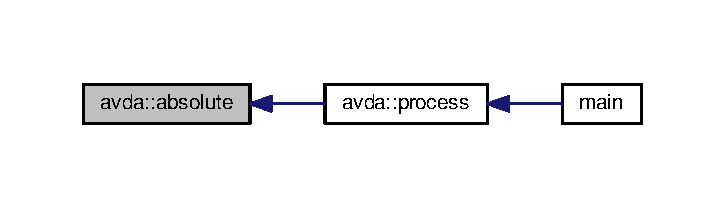
\includegraphics[width=348pt]{namespaceavda_aa771d0ed99fc4954c643ea71e91905bf_icgraph}
\end{center}
\end{figure}


\hypertarget{namespaceavda_a2a830f24a59aa2538ea82f6e000cce61}{\index{avda@{avda}!average@{average}}
\index{average@{average}!avda@{avda}}
\subsubsection[{average}]{\setlength{\rightskip}{0pt plus 5cm}{\bf float32} avda\+::average (
\begin{DoxyParamCaption}
\item[{{\bf float32} $\ast$}]{data, }
\item[{{\bf uint32}}]{size}
\end{DoxyParamCaption}
)}}\label{namespaceavda_a2a830f24a59aa2538ea82f6e000cce61}
Takes the average of all elements in an array


\begin{DoxyParams}{Parameters}
{\em data} & the array from which to compute the average\\
\hline
{\em size} & the number of elements in the data array\\
\hline
\end{DoxyParams}
\begin{DoxyReturn}{Returns}
the computed average 
\end{DoxyReturn}


Definition at line \hyperlink{sigmath_8hpp_source_l00129}{129} of file \hyperlink{sigmath_8hpp_source}{sigmath.\+hpp}.


\begin{DoxyCode}
00129                                                 \{
00130         \hyperlink{definitions_8hpp_aacdc525d6f7bddb3ae95d5c311bd06a1}{float32} ave;
00131 
00132         \textcolor{keywordflow}{for}(\hyperlink{definitions_8hpp_a1134b580f8da4de94ca6b1de4d37975e}{uint32} i = 0; i < size; i++) \{
00133             ave += data[i];
00134         \}
00135 
00136         ave = ave / size;
00137         \textcolor{keywordflow}{return} ave;
00138     \}
\end{DoxyCode}


Here is the caller graph for this function\+:
\nopagebreak
\begin{figure}[H]
\begin{center}
\leavevmode
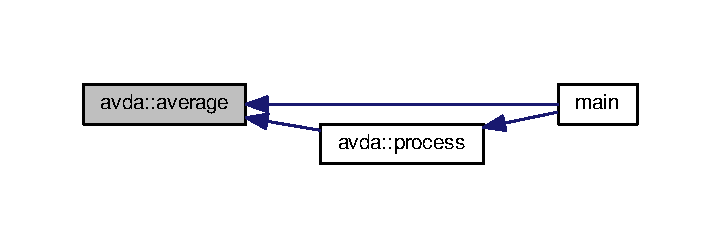
\includegraphics[width=346pt]{namespaceavda_a2a830f24a59aa2538ea82f6e000cce61_icgraph}
\end{center}
\end{figure}


\hypertarget{namespaceavda_a87927e04b25012fa7fa0fe05eefce41a}{\index{avda@{avda}!average@{average}}
\index{average@{average}!avda@{avda}}
\subsubsection[{average}]{\setlength{\rightskip}{0pt plus 5cm}{\bf Data\+Params} avda\+::average (
\begin{DoxyParamCaption}
\item[{{\bf Data\+Params} $\ast$}]{params, }
\item[{{\bf uint8}}]{size}
\end{DoxyParamCaption}
)}}\label{namespaceavda_a87927e04b25012fa7fa0fe05eefce41a}
Finds the averages of the elements of an array of \hyperlink{structDataParams}{Data\+Params}.


\begin{DoxyParams}{Parameters}
{\em params} & the \hyperlink{structDataParams}{Data\+Params} array\\
\hline
{\em size} & the number of elements in the \hyperlink{structDataParams}{Data\+Params} array\\
\hline
\end{DoxyParams}
\begin{DoxyReturn}{Returns}
a \hyperlink{structDataParams}{Data\+Params} structure containing the average values of the structure's elements in the params array 
\end{DoxyReturn}


Definition at line \hyperlink{sigmath_8hpp_source_l00140}{140} of file \hyperlink{sigmath_8hpp_source}{sigmath.\+hpp}.


\begin{DoxyCode}
00140                                                        \{
00141         \hyperlink{structDataParams}{DataParams} ave;
00142 
00143         \textcolor{keywordflow}{for}(\hyperlink{definitions_8hpp_adde6aaee8457bee49c2a92621fe22b79}{uint8} i = 0; i < size; i++) \{
00144             \textcolor{comment}{//freq is an attribute. this is how to add structure attributes}
00145             ave.\hyperlink{structDataParams_a12566e017407647bc8287d62554ad3fb}{freq} += params[i].\hyperlink{structDataParams_a12566e017407647bc8287d62554ad3fb}{freq};
00146             ave.\hyperlink{structDataParams_a4efd1d2231c6fa7c878c9d5e1650738f}{noise} += params[i].\hyperlink{structDataParams_a4efd1d2231c6fa7c878c9d5e1650738f}{noise};
00147         \}
00148 
00149         ave.\hyperlink{structDataParams_a12566e017407647bc8287d62554ad3fb}{freq} /= size;
00150         ave.\hyperlink{structDataParams_a4efd1d2231c6fa7c878c9d5e1650738f}{noise} /= size;
00151         \textcolor{keywordflow}{return} ave;
00152     \}
\end{DoxyCode}
\hypertarget{namespaceavda_a9c0b7f832eace3cbc9c5dddea2ecc9d5}{\index{avda@{avda}!decibels@{decibels}}
\index{decibels@{decibels}!avda@{avda}}
\subsubsection[{decibels}]{\setlength{\rightskip}{0pt plus 5cm}void avda\+::decibels (
\begin{DoxyParamCaption}
\item[{{\bf float32} $\ast$}]{data, }
\item[{{\bf uint32}}]{size}
\end{DoxyParamCaption}
)}}\label{namespaceavda_a9c0b7f832eace3cbc9c5dddea2ecc9d5}
Converts an array of floats to \char`\"{}power decibels\char`\"{}, i.\+e., x\mbox{[}n\mbox{]} = 20$\ast$log10(x\mbox{[}n\mbox{]}). The decibel values are written to the same array that contained the values to be converted. In other words, this function should perform an in-\/place, element-\/wise conversion.


\begin{DoxyParams}{Parameters}
{\em data} & the array of values to be converted as well as the location where the converted values will be written\\
\hline
{\em size} & the number of elements in the data array \\
\hline
\end{DoxyParams}


Definition at line \hyperlink{sigmath_8hpp_source_l00154}{154} of file \hyperlink{sigmath_8hpp_source}{sigmath.\+hpp}.


\begin{DoxyCode}
00154                                               \{
00155         \textcolor{keywordflow}{for}(\hyperlink{definitions_8hpp_a1134b580f8da4de94ca6b1de4d37975e}{uint32} i = 0; i < size; i++) \{
00156             data[i] = 20 * log10(data[i]);
00157         \}
00158     \}
\end{DoxyCode}


Here is the caller graph for this function\+:
\nopagebreak
\begin{figure}[H]
\begin{center}
\leavevmode
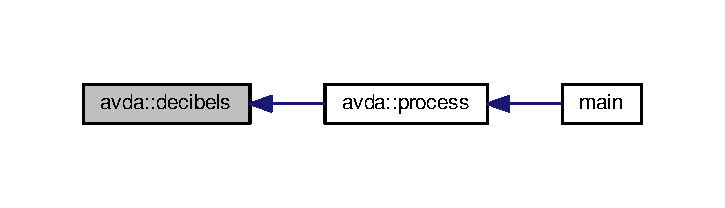
\includegraphics[width=348pt]{namespaceavda_a9c0b7f832eace3cbc9c5dddea2ecc9d5_icgraph}
\end{center}
\end{figure}


\hypertarget{namespaceavda_a3e9b92cfa9d76c4c363e8ed8a4c1a2ce}{\index{avda@{avda}!diff@{diff}}
\index{diff@{diff}!avda@{avda}}
\subsubsection[{diff}]{\setlength{\rightskip}{0pt plus 5cm}void avda\+::diff (
\begin{DoxyParamCaption}
\item[{{\bf float32} $\ast$}]{data, }
\item[{{\bf uint32}}]{size}
\end{DoxyParamCaption}
)}}\label{namespaceavda_a3e9b92cfa9d76c4c363e8ed8a4c1a2ce}
Computes the left-\/handed first derivative of a discrete signal. The first element will be 0.


\begin{DoxyParams}{Parameters}
{\em data} & an array containing the discrete signal data\\
\hline
{\em size} & the number of elements in data \\
\hline
\end{DoxyParams}


Definition at line \hyperlink{sigmath_8hpp_source_l00160}{160} of file \hyperlink{sigmath_8hpp_source}{sigmath.\+hpp}.


\begin{DoxyCode}
00160                                           \{
00161         \hyperlink{definitions_8hpp_aacdc525d6f7bddb3ae95d5c311bd06a1}{float32} temp[size];
00162         temp[0] = 0;
00163 
00164         \textcolor{keywordflow}{for}(\hyperlink{definitions_8hpp_a1134b580f8da4de94ca6b1de4d37975e}{uint32} i = 1; i < size; i++) \{
00165             temp[i] = data[i] - data[i-1];
00166         \}
00167 
00168         \textcolor{keywordflow}{for}(\hyperlink{definitions_8hpp_a1134b580f8da4de94ca6b1de4d37975e}{uint32} i = 0; i < size; i++) \{
00169             data[i] = temp[i];
00170         \}
00171     \}
\end{DoxyCode}


Here is the caller graph for this function\+:
\nopagebreak
\begin{figure}[H]
\begin{center}
\leavevmode
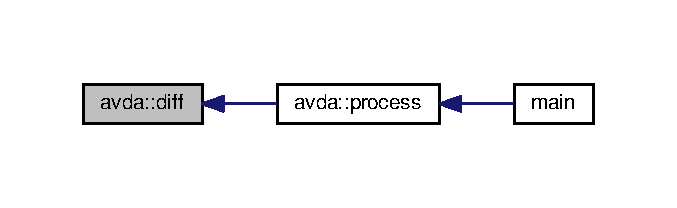
\includegraphics[width=325pt]{namespaceavda_a3e9b92cfa9d76c4c363e8ed8a4c1a2ce_icgraph}
\end{center}
\end{figure}


\hypertarget{namespaceavda_a33a1102422421212ac6b9387c896e864}{\index{avda@{avda}!fft@{fft}}
\index{fft@{fft}!avda@{avda}}
\subsubsection[{fft}]{\setlength{\rightskip}{0pt plus 5cm}void avda\+::fft (
\begin{DoxyParamCaption}
\item[{{\bf cfloat32} $\ast$}]{data, }
\item[{{\bf uint32}}]{size}
\end{DoxyParamCaption}
)}}\label{namespaceavda_a33a1102422421212ac6b9387c896e864}
Replaces the values of an array of cfloat32's with the array's D\+F\+T using a decimation-\/in-\/frequency algorithm.

This code is based on code from \href{http://rosettacode.org/wiki/Fast_Fourier_transform#C.2B.2B}{\tt http\+://rosettacode.\+org/wiki/\+Fast\+\_\+\+Fourier\+\_\+transform\#\+C.\+2\+B.\+2\+B}.


\begin{DoxyParams}{Parameters}
{\em data} & the array whose values should be replaced with its D\+F\+T\\
\hline
{\em size} & the number of elements in the data array \\
\hline
\end{DoxyParams}


Definition at line \hyperlink{sigmath_8hpp_source_l00173}{173} of file \hyperlink{sigmath_8hpp_source}{sigmath.\+hpp}.


\begin{DoxyCode}
00173                                           \{
00174         \textcolor{comment}{// DFT}
00175         \hyperlink{definitions_8hpp_a1134b580f8da4de94ca6b1de4d37975e}{uint32} k = size;
00176         \hyperlink{definitions_8hpp_a1134b580f8da4de94ca6b1de4d37975e}{uint32} n;
00177         \hyperlink{definitions_8hpp_aacdc525d6f7bddb3ae95d5c311bd06a1}{float32} thetaT = M\_PI / size;
00178         \hyperlink{definitions_8hpp_a960be6b6614c08090c16574dba10a421}{cfloat32} phiT(cos(thetaT), sin(thetaT));
00179         \hyperlink{definitions_8hpp_a960be6b6614c08090c16574dba10a421}{cfloat32} T;
00180 
00181         \textcolor{keywordflow}{while}(k > 1) \{
00182             n = k;
00183             k >>= 1;
00184             phiT = phiT * phiT;
00185             T = 1.0L;
00186 
00187             \textcolor{keywordflow}{for}(\hyperlink{definitions_8hpp_a1134b580f8da4de94ca6b1de4d37975e}{uint32} l = 0; l < k; l++) \{
00188                 \textcolor{keywordflow}{for}(\hyperlink{definitions_8hpp_a1134b580f8da4de94ca6b1de4d37975e}{uint32} a = l; a < size; a += n) \{
00189                     \hyperlink{definitions_8hpp_a1134b580f8da4de94ca6b1de4d37975e}{uint32} b = a + k;
00190                     \hyperlink{definitions_8hpp_a960be6b6614c08090c16574dba10a421}{cfloat32} t = data[a] - data[b];
00191                     data[a] += data[b];
00192                     data[b] = t * T;
00193                 \}
00194 
00195                 T *= phiT;
00196             \}
00197         \}
00198 
00199         \textcolor{comment}{// Decimate}
00200         \hyperlink{definitions_8hpp_a1134b580f8da4de94ca6b1de4d37975e}{uint32} m = (\hyperlink{definitions_8hpp_a1134b580f8da4de94ca6b1de4d37975e}{uint32})log2(size);
00201 
00202         \textcolor{keywordflow}{for}(\hyperlink{definitions_8hpp_a1134b580f8da4de94ca6b1de4d37975e}{uint32} a = 0; a < size; a++) \{
00203             \hyperlink{definitions_8hpp_a1134b580f8da4de94ca6b1de4d37975e}{uint32} b = a;
00204 
00205             \textcolor{comment}{// Reverse bits}
00206             b = (((b & 0xaaaaaaaa) >> 1) | ((b & 0x55555555) << 1));
00207             b = (((b & 0xcccccccc) >> 2) | ((b & 0x33333333) << 2));
00208             b = (((b & 0xf0f0f0f0) >> 4) | ((b & 0x0f0f0f0f) << 4));
00209             b = (((b & 0xff00ff00) >> 8) | ((b & 0x00ff00ff) << 8));
00210             b = ((b >> 16) | (b << 16)) >> (32 - m);
00211 
00212             \textcolor{keywordflow}{if} (b > a)
00213             \{
00214                 \hyperlink{definitions_8hpp_a960be6b6614c08090c16574dba10a421}{cfloat32} t = data[a];
00215                 data[a] = data[b];
00216                 data[b] = t;
00217             \}
00218         \}
00219     \}
\end{DoxyCode}


Here is the caller graph for this function\+:
\nopagebreak
\begin{figure}[H]
\begin{center}
\leavevmode
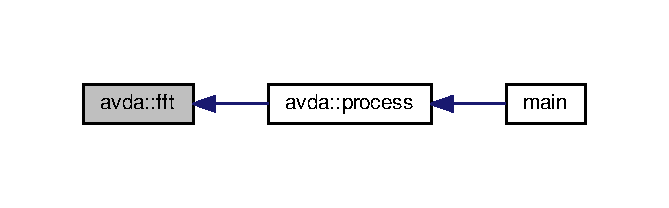
\includegraphics[width=321pt]{namespaceavda_a33a1102422421212ac6b9387c896e864_icgraph}
\end{center}
\end{figure}


\hypertarget{namespaceavda_a213bd6384fc9a330e4db2cecdbcd73ee}{\index{avda@{avda}!mag@{mag}}
\index{mag@{mag}!avda@{avda}}
\subsubsection[{mag}]{\setlength{\rightskip}{0pt plus 5cm}void avda\+::mag (
\begin{DoxyParamCaption}
\item[{{\bf cfloat32} $\ast$}]{orig, }
\item[{{\bf float32} $\ast$}]{newmags, }
\item[{{\bf uint32}}]{size}
\end{DoxyParamCaption}
)}}\label{namespaceavda_a213bd6384fc9a330e4db2cecdbcd73ee}
Computes the magitude of an array of complex numbers.


\begin{DoxyParams}{Parameters}
{\em orig} & the array of complex numbers\\
\hline
{\em newmags} & an array to which the magitudes are to be written\\
\hline
{\em size} & the number of elements in orig and newmags \\
\hline
\end{DoxyParams}


Definition at line \hyperlink{sigmath_8hpp_source_l00221}{221} of file \hyperlink{sigmath_8hpp_source}{sigmath.\+hpp}.


\begin{DoxyCode}
00221                                                             \{
00222         \textcolor{comment}{//loop to run throught the length of array orig}
00223         \textcolor{keywordflow}{for}(\hyperlink{definitions_8hpp_a1134b580f8da4de94ca6b1de4d37975e}{uint32} n = 0; n < size; n++) \{
00224             \textcolor{comment}{/* }
00225 \textcolor{comment}{             * abs should calculate the magnitude of complex array elements.}
00226 \textcolor{comment}{             * saves to new array}
00227 \textcolor{comment}{             */}
00228             newmags[n] = std::abs(orig[n]);     
00229         \}
00230     \}
\end{DoxyCode}


Here is the caller graph for this function\+:
\nopagebreak
\begin{figure}[H]
\begin{center}
\leavevmode
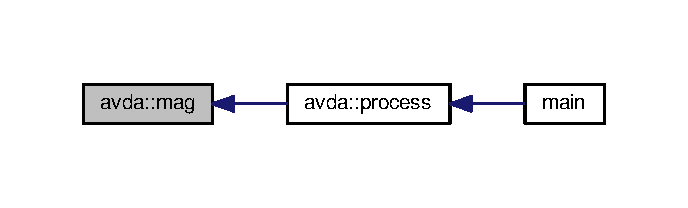
\includegraphics[width=330pt]{namespaceavda_a213bd6384fc9a330e4db2cecdbcd73ee_icgraph}
\end{center}
\end{figure}


\hypertarget{namespaceavda_aa82021c3ee552773c060b1a39caf8aaa}{\index{avda@{avda}!max@{max}}
\index{max@{max}!avda@{avda}}
\subsubsection[{max}]{\setlength{\rightskip}{0pt plus 5cm}{\bf Maximum} avda\+::max (
\begin{DoxyParamCaption}
\item[{{\bf float32} $\ast$}]{data, }
\item[{{\bf uint32}}]{size}
\end{DoxyParamCaption}
)}}\label{namespaceavda_aa82021c3ee552773c060b1a39caf8aaa}
Finds the maximum value in an array.


\begin{DoxyParams}{Parameters}
{\em data} & the array whose maximum value is to be found\\
\hline
{\em uint32} & size the number of elements in the data array\\
\hline
\end{DoxyParams}
\begin{DoxyReturn}{Returns}
the maximum value and its index in a \hyperlink{structMaximum}{Maximum} structure 
\end{DoxyReturn}


Definition at line \hyperlink{sigmath_8hpp_source_l00232}{232} of file \hyperlink{sigmath_8hpp_source}{sigmath.\+hpp}.


\begin{DoxyCode}
00232                                             \{
00233         \hyperlink{structMaximum}{Maximum} m;
00234 
00235         \textcolor{comment}{//loop to run through the length of array data}
00236         \textcolor{keywordflow}{for} (\hyperlink{definitions_8hpp_a1134b580f8da4de94ca6b1de4d37975e}{uint32} i = 0; i < size; i++) \{
00237             \textcolor{comment}{/* }
00238 \textcolor{comment}{             * when value at data[i] is above max.value,}
00239 \textcolor{comment}{             * sets max.value equal to data[i] and max.index equal to i}
00240 \textcolor{comment}{             */}
00241             \textcolor{keywordflow}{if} (data[i] > m.\hyperlink{structMaximum_aa7e84cbf37b694670142670014366969}{value}) \{
00242                 m.\hyperlink{structMaximum_aa7e84cbf37b694670142670014366969}{value} = data[i];
00243                 m.\hyperlink{structMaximum_a2e6aef03795cd285fe542d0861c6e3b5}{index} = i;
00244             \}
00245         \}
00246 
00247         \textcolor{keywordflow}{return} m;
00248     \}
\end{DoxyCode}


Here is the caller graph for this function\+:
\nopagebreak
\begin{figure}[H]
\begin{center}
\leavevmode
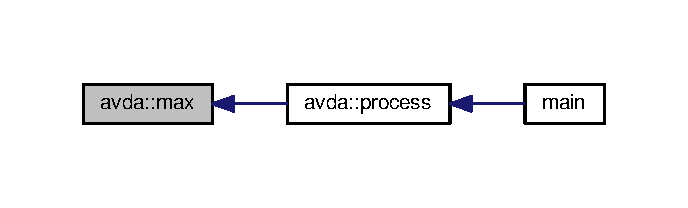
\includegraphics[width=330pt]{namespaceavda_aa82021c3ee552773c060b1a39caf8aaa_icgraph}
\end{center}
\end{figure}


\hypertarget{namespaceavda_ae20728e7e8ae50bf2f74849e538841ea}{\index{avda@{avda}!Patient\+Name@{Patient\+Name}}
\index{Patient\+Name@{Patient\+Name}!avda@{avda}}
\subsubsection[{Patient\+Name}]{\setlength{\rightskip}{0pt plus 5cm}std\+::string avda\+::\+Patient\+Name (
\begin{DoxyParamCaption}
{}
\end{DoxyParamCaption}
)}}\label{namespaceavda_ae20728e7e8ae50bf2f74849e538841ea}
Prompts a user to enter a first, middle, and last name for a patients and creates a file (if necessary) in which all of a patient's data can be saved. A newly created file will contain the C\+S\+V header for the file's data.

Must warn a user if the patient folder does not already exist in order to prevent missaving data.

\begin{DoxyReturn}{Returns}
the file under which all patient data is saved 
\end{DoxyReturn}


Definition at line \hyperlink{fileio_8hpp_source_l00043}{43} of file \hyperlink{fileio_8hpp_source}{fileio.\+hpp}.


\begin{DoxyCode}
00043                             \{
00044         std::string fname = \textcolor{stringliteral}{""};
00045         std::string mname = \textcolor{stringliteral}{""};
00046         std::string lname = \textcolor{stringliteral}{""};
00047         std::string patfil = \textcolor{stringliteral}{""};
00048         std::string patientname = \textcolor{stringliteral}{""};
00049         \hyperlink{definitions_8hpp_a1134b580f8da4de94ca6b1de4d37975e}{uint32} track1 = 0;
00050         \hyperlink{definitions_8hpp_a1134b580f8da4de94ca6b1de4d37975e}{uint32} track2 = 0;
00051         \hyperlink{definitions_8hpp_a1134b580f8da4de94ca6b1de4d37975e}{uint32} track3 = 0;
00052 
00053         \textcolor{keywordflow}{do} \{
00054             std::cout << \textcolor{stringliteral}{"Please enter the patients name."} << std::endl;
00055             std::cout << \textcolor{stringliteral}{"First name: "};
00056             std::cin >> fname;
00057             std::cout << \textcolor{stringliteral}{"Middle name: "};
00058             std::cin >> mname;
00059             std::cout << \textcolor{stringliteral}{"Last name: "};
00060             std::cin >> lname;
00061 
00062             \textcolor{comment}{// creates new std::string with path to patient file}
00063             patientname = \hyperlink{namespaceavda_a8ee73ec0cb55d4a13e89949764dce89d}{PATIENT\_PATH} + lname + \textcolor{stringliteral}{", "} + fname
00064                 + \textcolor{stringliteral}{" "} + mname + \textcolor{stringliteral}{".csv"};
00065 
00066             \textcolor{comment}{// prints out patientname. shows user the path to the patient file}
00067             \textcolor{comment}{//std::cout << patientname << std::endl << std::endl;}
00068             std::ifstream file(patientname.c\_str());
00069 
00070             \textcolor{keywordflow}{if} (file.good()) \{
00071                 track1 = 1;
00072             \}
00073 
00074             \textcolor{comment}{/*}
00075 \textcolor{comment}{             * Compares patientname to existing files and lets user know}
00076 \textcolor{comment}{             * if the file does not exist.}
00077 \textcolor{comment}{             */}
00078             \textcolor{keywordflow}{else} \textcolor{keywordflow}{if} (!file.good()) \{
00079                 \textcolor{comment}{/* }
00080 \textcolor{comment}{                 * Do while statement to continue asking user about the file}
00081 \textcolor{comment}{                 * if their input is not acceptable}
00082 \textcolor{comment}{                 */} 
00083                 \textcolor{keywordflow}{do} \{
00084                     std::cout << \textcolor{stringliteral}{"Patient file does not exist, would you like "}
00085                         \textcolor{stringliteral}{"to create file or re-enter their name?"} << std::endl;
00086                     std::cout << \textcolor{stringliteral}{"  *Type 'create' and press enter key "}
00087                         \textcolor{stringliteral}{"to create the patient file."} << std::endl;
00088                     std::cout << \textcolor{stringliteral}{"  *Type 'reenter' and press enter key "}
00089                         \textcolor{stringliteral}{"to re-enter the patients name."} << std::endl;
00090                     std::cout << std::endl;
00091                     std::cin >> patfil;
00092 
00093                     \textcolor{comment}{/* }
00094 \textcolor{comment}{                     * patfil equals create, track1 and 2 will increase}
00095 \textcolor{comment}{                     * escaping both do while loops}
00096 \textcolor{comment}{                     */}
00097                     \textcolor{keywordflow}{if}(patfil == \textcolor{stringliteral}{"create"}) \{
00098                         std::ofstream createfile(patientname.c\_str());
00099                         track1 = 1;
00100                         track2 = 1;
00101                         track3 = 1;
00102                         createfile << \hyperlink{namespaceavda_ac568a0872c2c176d874b8b12f67f43ea}{CSV\_HEADER} << std::endl;
00103                         createfile.flush();
00104                         createfile.close();
00105                     \}
00106 
00107                     \textcolor{comment}{/*}
00108 \textcolor{comment}{                     *patfil equals renter, track1 will remain zero allowing}
00109 \textcolor{comment}{                     *user to reenter the patient name.}
00110 \textcolor{comment}{                     */}
00111                     \textcolor{keywordflow}{else} \textcolor{keywordflow}{if}(patfil == \textcolor{stringliteral}{"reenter"}) \{
00112                         track1 = 0;
00113                         track2 = 1;
00114                     \}
00115 
00116                     \textcolor{comment}{/*}
00117 \textcolor{comment}{                     *The users input was neither create or reenter. User}
00118 \textcolor{comment}{                     *must enter patient name again.}
00119 \textcolor{comment}{                     */}
00120                     \textcolor{keywordflow}{else} \{
00121                         std::cout << std::endl;
00122                         std::cout << \textcolor{stringliteral}{"Your input is not acceptable."} << std::endl;
00123                         std::cout << std::endl;
00124                     \}
00125                 \}\textcolor{keywordflow}{while}(track2 == 0);
00126             \}
00127         \} \textcolor{keywordflow}{while} (track1 == 0);
00128 
00129         \textcolor{keywordflow}{return} patientname; \textcolor{comment}{//returns the path to the patient file}
00130     \}
\end{DoxyCode}


Here is the caller graph for this function\+:
\nopagebreak
\begin{figure}[H]
\begin{center}
\leavevmode
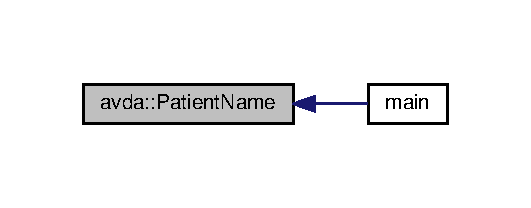
\includegraphics[width=255pt]{namespaceavda_ae20728e7e8ae50bf2f74849e538841ea_icgraph}
\end{center}
\end{figure}


\hypertarget{namespaceavda_a34f661f9a357bb68b0aa3662cc821e4d}{\index{avda@{avda}!play@{play}}
\index{play@{play}!avda@{avda}}
\subsubsection[{play}]{\setlength{\rightskip}{0pt plus 5cm}void avda\+::play (
\begin{DoxyParamCaption}
\item[{auto}]{filename}
\end{DoxyParamCaption}
)}}\label{namespaceavda_a34f661f9a357bb68b0aa3662cc821e4d}
Plays a W\+A\+V\+E file in a loop in a non-\/blocking manner.


\begin{DoxyParams}{Parameters}
{\em filename} & the absolute or relative path to the W\+A\+V\+E file \\
\hline
\end{DoxyParams}


Definition at line \hyperlink{sound_8hpp_source_l00020}{20} of file \hyperlink{sound_8hpp_source}{sound.\+hpp}.


\begin{DoxyCode}
00020                              \{
00021 
00022     \}
\end{DoxyCode}
\hypertarget{namespaceavda_a5196cce27286d08ca144a460caee7839}{\index{avda@{avda}!process@{process}}
\index{process@{process}!avda@{avda}}
\subsubsection[{process}]{\setlength{\rightskip}{0pt plus 5cm}{\bf Data\+Params} avda\+::process (
\begin{DoxyParamCaption}
\item[{{\bf float32} $\ast$}]{data, }
\item[{{\bf uint32}}]{size, }
\item[{{\bf float32}}]{sampling\+Rate}
\end{DoxyParamCaption}
)}}\label{namespaceavda_a5196cce27286d08ca144a460caee7839}
Analyzes a single recording to determine the drop-\/off frequency and average noiseband noise power.

It should be noted that is algorithm is considered the intellectual property of Andrew Wisner and Nicholas Nolan. The \char`\"{}algorithm\char`\"{} is defined as the use of 1) the frequency drop-\/off and/or 2) a noise value from the frequency band above the drop-\/off frequency in order to diagnose (with or without other factors and parameters) the presence of a avdaspasm in a patient. By faculty members and/or students in the U\+A\+B E\+C\+E department using this algorithm, they agree that the presentation of their code or project that uses this algorithm by anyone directly or indirectly related to the code or project, whether verbally or in writing, will reference the development of the initial algorithm by Andrew Wisner and Nicholas Nolan. Furthermore, a failure to meet this stipulation will warrant appropriate action by Andrew Wisner and/or Nicholas Nolan. It should be understood that the purpose of this stipulation is not to protect prioprietary rights; rather, it is to help ensure that the intellectual property of the aforementioned is protected and is neither misrepresented nor claimed implicitly or explicitly by another individual.


\begin{DoxyParams}{Parameters}
{\em data} & array containing float32 samples of audio\\
\hline
{\em size} & number of samples in each recording. M\+U\+S\+T be a power of two.\\
\hline
{\em sampling\+Rate} & the sampling frequency in Hz or Samples/second\\
\hline
\end{DoxyParams}
\begin{DoxyReturn}{Returns}
cut-\/off frequency (Hz) and average noiseband noise power in decibels 
\end{DoxyReturn}


Definition at line \hyperlink{process_8hpp_source_l00048}{48} of file \hyperlink{process_8hpp_source}{process.\+hpp}.


\begin{DoxyCode}
00048                                                                          \{
00049         \textcolor{keywordflow}{if}((size & (size - 1) != 0) || size < 2) \{
00050             \textcolor{keywordflow}{throw} std::invalid\_argument(
00051                     \textcolor{stringliteral}{"The number of samples is not a power of two!"});
00052         \}
00053 
00054         \textcolor{comment}{// declare function-scoped variables}
00055         \hyperlink{definitions_8hpp_a1134b580f8da4de94ca6b1de4d37975e}{uint32} freqSize = size / 2;
00056         \hyperlink{definitions_8hpp_a960be6b6614c08090c16574dba10a421}{cfloat32}* cdata = (\hyperlink{definitions_8hpp_a960be6b6614c08090c16574dba10a421}{cfloat32}*)std::malloc(size * \textcolor{keyword}{sizeof}(
      \hyperlink{definitions_8hpp_a960be6b6614c08090c16574dba10a421}{cfloat32}));
00057         \hyperlink{definitions_8hpp_aacdc525d6f7bddb3ae95d5c311bd06a1}{float32}* fdata = (\hyperlink{definitions_8hpp_aacdc525d6f7bddb3ae95d5c311bd06a1}{float32}*)std::malloc(freqSize * \textcolor{keyword}{sizeof}(
      \hyperlink{definitions_8hpp_aacdc525d6f7bddb3ae95d5c311bd06a1}{float32}));
00058         \hyperlink{definitions_8hpp_aacdc525d6f7bddb3ae95d5c311bd06a1}{float32}* origdata = (\hyperlink{definitions_8hpp_aacdc525d6f7bddb3ae95d5c311bd06a1}{float32}*)std::malloc(freqSize * \textcolor{keyword}{sizeof}(
      \hyperlink{definitions_8hpp_aacdc525d6f7bddb3ae95d5c311bd06a1}{float32}));
00059 
00060         \textcolor{comment}{// convert data to complex numbers for fft()}
00061         \textcolor{keywordflow}{for}(\hyperlink{definitions_8hpp_a1134b580f8da4de94ca6b1de4d37975e}{uint32} i = 0; i < size; i++) \{
00062             cdata[i] = data[i];
00063         \}
00064     
00065         \textcolor{comment}{// find frequency spectrum in relative decibels}
00066         \hyperlink{namespaceavda_a33a1102422421212ac6b9387c896e864}{fft}(cdata, size);
00067         \hyperlink{namespaceavda_a213bd6384fc9a330e4db2cecdbcd73ee}{mag}(cdata, fdata, freqSize);
00068         \hyperlink{structMaximum}{Maximum} maximum = \hyperlink{namespaceavda_aa82021c3ee552773c060b1a39caf8aaa}{max}(fdata, freqSize);
00069 
00070         \textcolor{keywordflow}{for}(\hyperlink{definitions_8hpp_a1134b580f8da4de94ca6b1de4d37975e}{uint32} i = 0; i < freqSize; i++) \{
00071             fdata[i] /= maximum.\hyperlink{structMaximum_aa7e84cbf37b694670142670014366969}{value};
00072         \}
00073 
00074         \hyperlink{namespaceavda_a9c0b7f832eace3cbc9c5dddea2ecc9d5}{decibels}(fdata, freqSize);
00075 
00076         \textcolor{keywordflow}{for}(\hyperlink{definitions_8hpp_a1134b580f8da4de94ca6b1de4d37975e}{uint32} i = 0; i < freqSize; i++) \{
00077             origdata[i] = fdata[i];
00078         \}
00079 
00080         \textcolor{comment}{/*}
00081 \textcolor{comment}{         * Run spectrum values through moving-average filter to smooth the}
00082 \textcolor{comment}{         * curve and make it easier to determine the derivative.}
00083 \textcolor{comment}{         */}
00084         \hyperlink{namespaceavda_a22583ba7f11b69c955b13155bf9a739d}{smooth}(fdata, freqSize, 20);
00085 
00086         \textcolor{comment}{/*}
00087 \textcolor{comment}{         * Find the derivative of the smoothed spectrum. Bote that both this}
00088 \textcolor{comment}{         * filter and the previous are necessary to the algorithm.}
00089 \textcolor{comment}{         */}
00090         \hyperlink{namespaceavda_a3e9b92cfa9d76c4c363e8ed8a4c1a2ce}{diff}(fdata, freqSize);
00091         \hyperlink{namespaceavda_a22583ba7f11b69c955b13155bf9a739d}{smooth}(fdata, freqSize, 100);
00092         \hyperlink{namespaceavda_aa771d0ed99fc4954c643ea71e91905bf}{absolute}(fdata, freqSize);
00093 
00094         \textcolor{comment}{// find the parameters of this specific recording}
00095         \hyperlink{definitions_8hpp_a05f6b0ae8f6a6e135b0e290c25fe0e4e}{uint16} offset = 1000;
00096         \hyperlink{namespaceavda_aa771d0ed99fc4954c643ea71e91905bf}{absolute}(&fdata[offset], freqSize - offset);
00097         maximum = \hyperlink{namespaceavda_aa82021c3ee552773c060b1a39caf8aaa}{max}(&fdata[offset], freqSize - offset);
00098         \hyperlink{definitions_8hpp_a1134b580f8da4de94ca6b1de4d37975e}{uint32} index = maximum.\hyperlink{structMaximum_a2e6aef03795cd285fe542d0861c6e3b5}{index} + offset;
00099         
00100         \hyperlink{structDataParams}{DataParams} params;
00101         params.\hyperlink{structDataParams_a12566e017407647bc8287d62554ad3fb}{freq} = index * (float)\hyperlink{definitions_8hpp_a8ace559345ecba7978591ac2ef22aea4}{SAMPLE\_FREQ} / freqSize / 2;
00102         params.\hyperlink{structDataParams_a4efd1d2231c6fa7c878c9d5e1650738f}{noise} = \hyperlink{namespaceavda_a2a830f24a59aa2538ea82f6e000cce61}{average}(&origdata[index + offset],
00103                 freqSize - offset - index);
00104 
00105         free(cdata);
00106         free(fdata);
00107 
00108         \textcolor{keywordflow}{return} params;
00109 
00110     \}
\end{DoxyCode}


Here is the call graph for this function\+:
\nopagebreak
\begin{figure}[H]
\begin{center}
\leavevmode
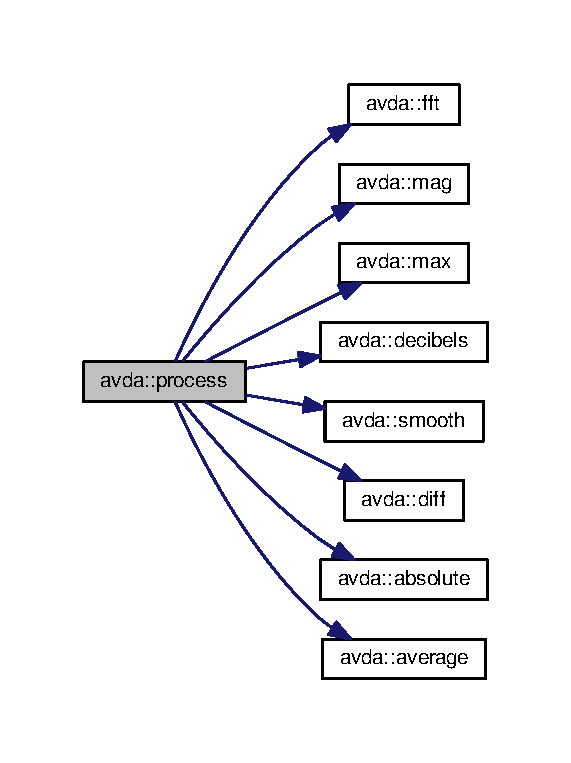
\includegraphics[width=274pt]{namespaceavda_a5196cce27286d08ca144a460caee7839_cgraph}
\end{center}
\end{figure}




Here is the caller graph for this function\+:
\nopagebreak
\begin{figure}[H]
\begin{center}
\leavevmode
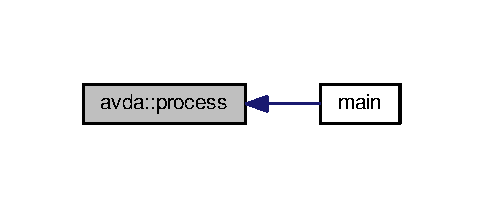
\includegraphics[width=232pt]{namespaceavda_a5196cce27286d08ca144a460caee7839_icgraph}
\end{center}
\end{figure}


\hypertarget{namespaceavda_a46dc980b65ddfc24749ce25c1290e158}{\index{avda@{avda}!Read\+Params@{Read\+Params}}
\index{Read\+Params@{Read\+Params}!avda@{avda}}
\subsubsection[{Read\+Params}]{\setlength{\rightskip}{0pt plus 5cm}std\+::map$<${\bf Side}, {\bf Data\+Params}$>$ avda\+::\+Read\+Params (
\begin{DoxyParamCaption}
\item[{auto}]{filename}
\end{DoxyParamCaption}
)}}\label{namespaceavda_a46dc980b65ddfc24749ce25c1290e158}
Reads the previously computated parameters found in the specified file.


\begin{DoxyParams}{Parameters}
{\em filename} & the absolute or relative path to the file containing the patient data to read\\
\hline
\end{DoxyParams}
\begin{DoxyReturn}{Returns}
the patient parameters read for each side 
\end{DoxyReturn}


Definition at line \hyperlink{fileio_8hpp_source_l00141}{141} of file \hyperlink{fileio_8hpp_source}{fileio.\+hpp}.


\begin{DoxyCode}
00141                                                        \{
00142         std::map<Side, DataParams> myMap;
00143         \hyperlink{structDataParams}{DataParams} leftparams;
00144         \hyperlink{structDataParams}{DataParams} rightparams;
00145 
00146         std::ifstream file(filename.c\_str());
00147         std::string leftline;
00148         std::string rightline;
00149         std::string leftsearch = \textcolor{stringliteral}{"Left"};
00150         std::string rightsearch = \textcolor{stringliteral}{"Right"};
00151         std::string paramstring;
00152         std::string lfreqstr;
00153         std::string lnoisestr;
00154         std::string rfreqstr;
00155         std::string rnoisestr;
00156         \hyperlink{definitions_8hpp_a1134b580f8da4de94ca6b1de4d37975e}{uint32} lcnt = 0;
00157         \hyperlink{definitions_8hpp_a1134b580f8da4de94ca6b1de4d37975e}{uint32} rcnt = 0;
00158         \hyperlink{definitions_8hpp_aacdc525d6f7bddb3ae95d5c311bd06a1}{float32} lfreqval;
00159         \hyperlink{definitions_8hpp_aacdc525d6f7bddb3ae95d5c311bd06a1}{float32} lnoiseval;
00160         \hyperlink{definitions_8hpp_aacdc525d6f7bddb3ae95d5c311bd06a1}{float32} rfreqval;
00161         \hyperlink{definitions_8hpp_aacdc525d6f7bddb3ae95d5c311bd06a1}{float32} rnoiseval;
00162 
00163         \textcolor{comment}{/*}
00164 \textcolor{comment}{         * if statement which uses ifstream function to open patient file }
00165 \textcolor{comment}{         * filename)}
00166 \textcolor{comment}{         */}
00167         \textcolor{keywordflow}{if}(file.is\_open()) \{
00168             \textcolor{comment}{/*}
00169 \textcolor{comment}{             * While statement to find the first Left line and save to }
00170 \textcolor{comment}{             *leftline as string.}
00171 \textcolor{comment}{             */}
00172             \textcolor{keywordflow}{while} (getline(file, leftline)) \{
00173                 \textcolor{keywordflow}{if}(leftline.find(leftsearch, 0) != std::string::npos) \{
00174                     \textcolor{keywordflow}{break};
00175                 \}
00176 
00177             \}
00178 
00179             \textcolor{comment}{/*}
00180 \textcolor{comment}{             * While statement to find first right line and save to rightline}
00181 \textcolor{comment}{             * as string.}
00182 \textcolor{comment}{             */}
00183             \textcolor{keywordflow}{while} (getline(file,rightline)) \{
00184                 \textcolor{keywordflow}{if}(rightline.find(rightsearch, 0) != std::string::npos) \{
00185                     \textcolor{keywordflow}{break};
00186                 \}
00187             \}
00188 
00189             \textcolor{comment}{// Code to break leftline and rightline into its parts}
00190             std::stringstream lss(leftline);
00191             std::stringstream rss(rightline);
00192 
00193             \textcolor{keywordflow}{while}(getline(lss,paramstring, \textcolor{charliteral}{','})) \{
00194                 lcnt++;
00195 
00196                 \textcolor{keywordflow}{if}(lcnt == 3) \{
00197                     lfreqstr = paramstring;
00198                 \}
00199 
00200                 \textcolor{keywordflow}{else} \textcolor{keywordflow}{if}(lcnt == 4) \{
00201                     lnoisestr = paramstring;
00202                 \}
00203             \}
00204 
00205             \textcolor{keywordflow}{while}(getline(rss,paramstring, \textcolor{charliteral}{','})) \{
00206                 rcnt++;
00207 
00208                 \textcolor{keywordflow}{if}(rcnt == 3) \{
00209                     rfreqstr = paramstring;
00210                 \}
00211 
00212                 \textcolor{keywordflow}{else} \textcolor{keywordflow}{if}(rcnt == 4) \{
00213                     rnoisestr = paramstring;
00214                 \}
00215             \}
00216 
00217             \textcolor{comment}{/*}
00218 \textcolor{comment}{             * Statement to convert lfreq, lnoise, rfreq, and rnoise from}
00219 \textcolor{comment}{             * strings to floats.}
00220 \textcolor{comment}{             * */}
00221             lfreqval = atof(lfreqstr.c\_str());
00222             lnoiseval = atof(lnoisestr.c\_str());
00223             rfreqval = atof(rfreqstr.c\_str());
00224             rnoiseval = atof(rnoisestr.c\_str());
00225 
00226             file.close();
00227         \}
00228 
00229         \textcolor{keywordflow}{else} \{
00230             \textcolor{keywordflow}{throw} std::runtime\_error(\textcolor{stringliteral}{"The patient file could not be opened."});
00231         \}
00232 
00233         leftparams.\hyperlink{structDataParams_a12566e017407647bc8287d62554ad3fb}{freq} = lfreqval;
00234         leftparams.\hyperlink{structDataParams_a4efd1d2231c6fa7c878c9d5e1650738f}{noise} = lnoiseval;
00235         rightparams.\hyperlink{structDataParams_a12566e017407647bc8287d62554ad3fb}{freq} = rfreqval;
00236         rightparams.\hyperlink{structDataParams_a4efd1d2231c6fa7c878c9d5e1650738f}{noise} = rnoiseval;
00237 
00238         myMap[Side::Left] = leftparams;
00239         myMap[Side::Right] = rightparams;
00240 
00241         \textcolor{keywordflow}{return} myMap;
00242     \}
\end{DoxyCode}


Here is the caller graph for this function\+:
\nopagebreak
\begin{figure}[H]
\begin{center}
\leavevmode
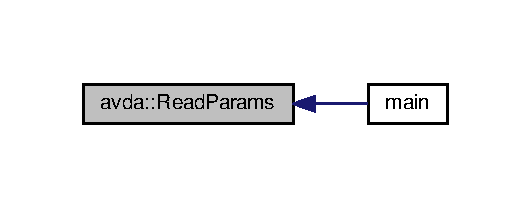
\includegraphics[width=255pt]{namespaceavda_a46dc980b65ddfc24749ce25c1290e158_icgraph}
\end{center}
\end{figure}


\hypertarget{namespaceavda_a22583ba7f11b69c955b13155bf9a739d}{\index{avda@{avda}!smooth@{smooth}}
\index{smooth@{smooth}!avda@{avda}}
\subsubsection[{smooth}]{\setlength{\rightskip}{0pt plus 5cm}void avda\+::smooth (
\begin{DoxyParamCaption}
\item[{{\bf float32} $\ast$}]{data, }
\item[{{\bf uint32}}]{size, }
\item[{{\bf uint16}}]{order}
\end{DoxyParamCaption}
)}}\label{namespaceavda_a22583ba7f11b69c955b13155bf9a739d}
Applies an nth-\/order moving-\/average filter to a discrete signal.


\begin{DoxyParams}{Parameters}
{\em data} & the array containing the signal to which the filter should be applied\\
\hline
{\em size} & the number of elements in the data array\\
\hline
{\em order} & the order of the filter \\
\hline
\end{DoxyParams}


Definition at line \hyperlink{sigmath_8hpp_source_l00250}{250} of file \hyperlink{sigmath_8hpp_source}{sigmath.\+hpp}.


\begin{DoxyCode}
00250                                                           \{
00251         \hyperlink{definitions_8hpp_aacdc525d6f7bddb3ae95d5c311bd06a1}{float32} coeff = 1 / (\hyperlink{definitions_8hpp_aacdc525d6f7bddb3ae95d5c311bd06a1}{float32})order;
00252         \hyperlink{definitions_8hpp_aacdc525d6f7bddb3ae95d5c311bd06a1}{float32} temp[size];
00253 
00254         \textcolor{keywordflow}{for}(\hyperlink{definitions_8hpp_a1134b580f8da4de94ca6b1de4d37975e}{uint32} i = 0; i < size; i++) \{
00255             temp[i] = 0;
00256 
00257             \textcolor{keywordflow}{for}(\hyperlink{definitions_8hpp_a05f6b0ae8f6a6e135b0e290c25fe0e4e}{uint16} j = 0; j < order && j <= i; j++) \{
00258                 temp[i] += data[i - j];
00259             \}
00260 
00261             temp[i] *= coeff;
00262         \}
00263 
00264         \textcolor{keywordflow}{for}(\hyperlink{definitions_8hpp_a1134b580f8da4de94ca6b1de4d37975e}{uint32} i = 0; i < size; i++) \{
00265             data[i] = temp[i];
00266         \}
00267     \}
\end{DoxyCode}


Here is the caller graph for this function\+:
\nopagebreak
\begin{figure}[H]
\begin{center}
\leavevmode
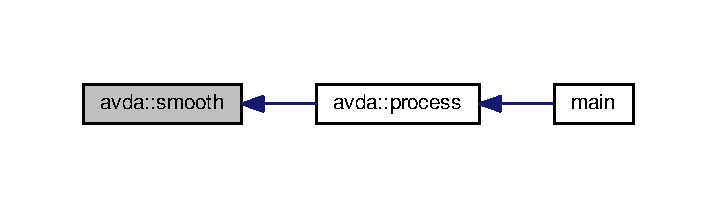
\includegraphics[width=344pt]{namespaceavda_a22583ba7f11b69c955b13155bf9a739d_icgraph}
\end{center}
\end{figure}


\hypertarget{namespaceavda_aba04a08b41833ced32ec803d55a63bee}{\index{avda@{avda}!Write\+Params@{Write\+Params}}
\index{Write\+Params@{Write\+Params}!avda@{avda}}
\subsubsection[{Write\+Params}]{\setlength{\rightskip}{0pt plus 5cm}void avda\+::\+Write\+Params (
\begin{DoxyParamCaption}
\item[{std\+::map$<$ Side, {\bf Data\+Params} $>$}]{my\+Map, }
\item[{auto}]{filename}
\end{DoxyParamCaption}
)}}\label{namespaceavda_aba04a08b41833ced32ec803d55a63bee}
Writes (appends) the passed parameters to the specified file.


\begin{DoxyParams}{Parameters}
{\em my\+Map} & contains the parameters to be written\\
\hline
\end{DoxyParams}
the patient C\+S\+V file's filename 

Definition at line \hyperlink{fileio_8hpp_source_l00251}{251} of file \hyperlink{fileio_8hpp_source}{fileio.\+hpp}.


\begin{DoxyCode}
00251                                                                     \{
00252         \textcolor{keywordtype}{char} temp[80];
00253         std::ofstream file(filename.c\_str(),
00254                 std::ofstream::out | std::ofstream::app);
00255 
00256         \textcolor{comment}{//Gives pointer measurementtime a data type of time\_t.}
00257         time\_t measurementtime;
00258         time(&measurementtime); \textcolor{comment}{//Gets the current time.}
00259         strftime(temp, 80, \textcolor{stringliteral}{"%c"}, localtime(&measurementtime));
00260         std::string fTime = std::string(temp);
00261 
00262         \textcolor{comment}{//if statement to print the Left side parameters to the patient file.}
00263         \textcolor{keywordflow}{if}(file.is\_open()) \{
00264             file << fTime + \textcolor{stringliteral}{","} + \textcolor{stringliteral}{"Left"} + \textcolor{stringliteral}{","}
00265                 + std::to\_string(myMap[Side::Left].freq) 
00266                 + \textcolor{stringliteral}{", "} + std::to\_string(myMap[Side::Left].noise) << std::endl;
00267         \}
00268 
00269         \textcolor{comment}{//if statement to print the Right side parameters to the patient file.}
00270         \textcolor{keywordflow}{if}(file.is\_open()) \{
00271             file << fTime + \textcolor{stringliteral}{","} + \textcolor{stringliteral}{"Right"} + \textcolor{stringliteral}{","}
00272                 + std::to\_string(myMap[Side::Right].freq) 
00273                 + \textcolor{stringliteral}{", "} + std::to\_string(myMap[Side::Right].noise) << std::endl;
00274         \}
00275 
00276         \textcolor{keywordflow}{else} \{
00277             std::cout << \textcolor{stringliteral}{"Patient file can not be opened!"} << std::endl;
00278         \}
00279 
00280         file.close();
00281     \}
\end{DoxyCode}


Here is the caller graph for this function\+:
\nopagebreak
\begin{figure}[H]
\begin{center}
\leavevmode
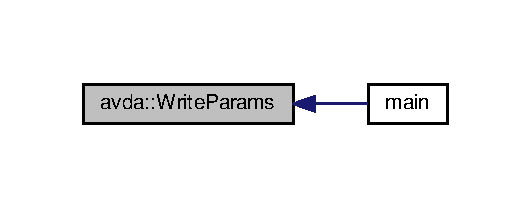
\includegraphics[width=255pt]{namespaceavda_aba04a08b41833ced32ec803d55a63bee_icgraph}
\end{center}
\end{figure}




\subsection{Variable Documentation}
\hypertarget{namespaceavda_ac568a0872c2c176d874b8b12f67f43ea}{\index{avda@{avda}!C\+S\+V\+\_\+\+H\+E\+A\+D\+E\+R@{C\+S\+V\+\_\+\+H\+E\+A\+D\+E\+R}}
\index{C\+S\+V\+\_\+\+H\+E\+A\+D\+E\+R@{C\+S\+V\+\_\+\+H\+E\+A\+D\+E\+R}!avda@{avda}}
\subsubsection[{C\+S\+V\+\_\+\+H\+E\+A\+D\+E\+R}]{\setlength{\rightskip}{0pt plus 5cm}const std\+::string avda\+::\+C\+S\+V\+\_\+\+H\+E\+A\+D\+E\+R = \char`\"{}Time,{\bf Side},Frequency,Noise Level\char`\"{}}}\label{namespaceavda_ac568a0872c2c176d874b8b12f67f43ea}
First line of C\+S\+V data file, which declares columns. 

Definition at line \hyperlink{fileio_8hpp_source_l00025}{25} of file \hyperlink{fileio_8hpp_source}{fileio.\+hpp}.

\hypertarget{namespaceavda_a8ee73ec0cb55d4a13e89949764dce89d}{\index{avda@{avda}!P\+A\+T\+I\+E\+N\+T\+\_\+\+P\+A\+T\+H@{P\+A\+T\+I\+E\+N\+T\+\_\+\+P\+A\+T\+H}}
\index{P\+A\+T\+I\+E\+N\+T\+\_\+\+P\+A\+T\+H@{P\+A\+T\+I\+E\+N\+T\+\_\+\+P\+A\+T\+H}!avda@{avda}}
\subsubsection[{P\+A\+T\+I\+E\+N\+T\+\_\+\+P\+A\+T\+H}]{\setlength{\rightskip}{0pt plus 5cm}const std\+::string avda\+::\+P\+A\+T\+I\+E\+N\+T\+\_\+\+P\+A\+T\+H = \char`\"{}/home/pi/patients/\char`\"{}}}\label{namespaceavda_a8ee73ec0cb55d4a13e89949764dce89d}
Absolute path to the folder containing the patients' data 

Definition at line \hyperlink{fileio_8hpp_source_l00030}{30} of file \hyperlink{fileio_8hpp_source}{fileio.\+hpp}.


\chapter{Class Documentation}
\hypertarget{structDataParams}{\section{Data\+Params Struct Reference}
\label{structDataParams}\index{Data\+Params@{Data\+Params}}
}


{\ttfamily \#include $<$definitions.\+hpp$>$}



\subsection{Detailed Description}
A structure containing the calculated results from processing the audio recordings. 

Definition at line 40 of file definitions.\+hpp.



The documentation for this struct was generated from the following file\+:\begin{DoxyCompactItemize}
\item 
src/\hyperlink{definitions_8hpp}{definitions.\+hpp}\end{DoxyCompactItemize}

\hypertarget{structMaximum}{\section{Maximum Struct Reference}
\label{structMaximum}\index{Maximum@{Maximum}}
}


{\ttfamily \#include $<$definitions.\+hpp$>$}

\subsection*{Public Attributes}
\begin{DoxyCompactItemize}
\item 
\hyperlink{definitions_8hpp_aacdc525d6f7bddb3ae95d5c311bd06a1}{float32} \hyperlink{structMaximum_aa7e84cbf37b694670142670014366969}{value}
\item 
\hyperlink{definitions_8hpp_a1134b580f8da4de94ca6b1de4d37975e}{uint32} \hyperlink{structMaximum_a2e6aef03795cd285fe542d0861c6e3b5}{index}
\end{DoxyCompactItemize}


\subsection{Detailed Description}
Contains the maximum value found in an array and the value's index in that array. 

Definition at line \hyperlink{definitions_8hpp_source_l00053}{53} of file \hyperlink{definitions_8hpp_source}{definitions.\+hpp}.



\subsection{Member Data Documentation}
\hypertarget{structMaximum_a2e6aef03795cd285fe542d0861c6e3b5}{\index{Maximum@{Maximum}!index@{index}}
\index{index@{index}!Maximum@{Maximum}}
\subsubsection[{index}]{\setlength{\rightskip}{0pt plus 5cm}{\bf uint32} Maximum\+::index}}\label{structMaximum_a2e6aef03795cd285fe542d0861c6e3b5}


Definition at line \hyperlink{definitions_8hpp_source_l00055}{55} of file \hyperlink{definitions_8hpp_source}{definitions.\+hpp}.

\hypertarget{structMaximum_aa7e84cbf37b694670142670014366969}{\index{Maximum@{Maximum}!value@{value}}
\index{value@{value}!Maximum@{Maximum}}
\subsubsection[{value}]{\setlength{\rightskip}{0pt plus 5cm}{\bf float32} Maximum\+::value}}\label{structMaximum_aa7e84cbf37b694670142670014366969}


Definition at line \hyperlink{definitions_8hpp_source_l00054}{54} of file \hyperlink{definitions_8hpp_source}{definitions.\+hpp}.



The documentation for this struct was generated from the following file\+:\begin{DoxyCompactItemize}
\item 
src/\hyperlink{definitions_8hpp}{definitions.\+hpp}\end{DoxyCompactItemize}

\chapter{File Documentation}
\hypertarget{doxygen_8config}{\section{etc/doxygen.config File Reference}
\label{doxygen_8config}\index{etc/doxygen.\+config@{etc/doxygen.\+config}}
}

\hypertarget{doxygen_8config_source}{\section{doxygen.\+config}
\label{doxygen_8config_source}\index{etc/doxygen.\+config@{etc/doxygen.\+config}}
}

\begin{DoxyCode}
00001 PROJECT\_NAME = "Andrew and Nick's Project"
00002 
00003 INPUT = src/ etc/doxygen.config makefile 
00004 OUTPUT\_DIRECTORY = doc/
00005 
00006 GENERATE\_HTML = YES
00007 GENERATE\_RTF = YES
00008 GENERATE\_LATEX = YES
00009 GENERATE\_MAN = YES
00010 GENERATE\_XML = NO
00011 GENERATE\_DOCBOOK = NO
00012 
00013 USE\_PDF\_LATEX = YES
00014 USE\_PDF\_HYPERLINKS = YES
00015 
00016 RECURSIVE = YES
00017 SOURCE\_BROWSER = YES
00018 SOURCE\_TOOLTIPS = YES
00019 EXTRACT\_ALL = YES
00020 DISABLE\_INDEX = NO
00021 GENERATE\_TREEVIEW = YES
00022 SEARCHENGINE = YES
00023 SERVER\_BASED\_SEARCH = NO
00024 
00025 LATEX\_SOURCE\_CODE = YES
00026 STRIP\_CODE\_COMMENTS = YES
00027 INLINE\_SOURCES = YES
00028 
00029 HAVE\_DOT = YES
00030 CALL\_GRAPH = YES
00031 CALLER\_GRAPH = YES
\end{DoxyCode}

\hypertarget{makefile}{\section{makefile File Reference}
\label{makefile}\index{makefile@{makefile}}
}


Contains recipes for building the test applications, the main application, and the documentation.  




\subsection{Detailed Description}
Contains recipes for building the test applications, the main application, and the documentation. 

\begin{DoxyAuthor}{Author}
Samuel Andrew Wisner, \href{mailto:awisner94@gmail.com}{\tt awisner94@gmail.\+com} 
\end{DoxyAuthor}


Definition in file \hyperlink{makefile_source}{makefile}.


\hypertarget{makefile_source}{\section{makefile}
}

\begin{DoxyCode}
00001 GCC = g++ -g -std=gnu++14
00002 
00003 avda:
00004    $(GCC) src/main.cpp -o bin/avda
00005 
00006 count:
00007    grep -r "src/" -e "Samuel Andrew Wisner" -l | xargs wc -l
00008 
00009 docs:
00010    rm -r doc/
00011    doxygen etc/doxygen.config
00012    cd doc/latex; make pdf;
00013    git reset
00014    git add doc/.
00015    git commit -m "Updated documentation."
00016    git push
00017 
00018 fileio-test:
00019    $(GCC) src/fileio\_test.cpp -o bin/fileiotest
00020 
00021 patient-name-test:
00022    $(GCC) src/patient\_name\_test.cpp -o bin/patnametest
00023 
00024 process-test:
00025    $(GCC) src/process\_test.cpp -o bin/proctest
00026 
00027 read-params-test:
00028    $(GCC) src/read\_params\_test.cpp -o bin/rptest
00029 
00030 stdin-clear-test:
00031    $(GCC) src/stdin\_clear\_test.cpp -o bin/cleartest
\end{DoxyCode}

\hypertarget{README_8md}{\section{R\+E\+A\+D\+M\+E.\+md File Reference}
\label{README_8md}\index{R\+E\+A\+D\+M\+E.\+md@{R\+E\+A\+D\+M\+E.\+md}}
}


Contains the readme text as markdown, which also doubles as the main page.  




\subsection{Detailed Description}
Contains the readme text as markdown, which also doubles as the main page. 

\begin{DoxyAuthor}{Author}
Samuel Andrew Wisner, \href{mailto:awisner94@gmail.com}{\tt awisner94@gmail.\+com} 
\end{DoxyAuthor}


Definition in file \hyperlink{README_8md_source}{R\+E\+A\+D\+M\+E.\+md}.


\hypertarget{README_8md_source}{\section{R\+E\+A\+D\+M\+E.\+md}
}

\begin{DoxyCode}
00001 # vasospasm-detector
00002 
00003 ## Introduction
00004 The Automatic Vasospasm Detection Application (or Algorithm, depending on the
00005 usage), AVDA, is an application to objectively detect the presence of vasospasms
00006 based on comparisons of parameters extracted from transcranial doppler audio.
00007 
00008 ## Setup
00009 AVDA is intended to be compiled on machines running Linux, though it could
00010 likely be adapter for other environments. It must be downloaded from GitHub.com
00011 and compiled locally. To do this, navigate to the directory in which AVDA should
00012 be placed, then execute the following commands
00013 
00014    git clone https://github.com/sawbg/avda
00015    cd avda
00016    make
00017 
00018 Sucessfully cloning, compilation, and execution of AVDA requires up-to-date
00019 versions of the following executables:
00020 
00021 * git
00022 * make
00023 * gcc (4.9)
00024 * arecord
00025 
00026 ## FAQ
00027 
00028 * **Why was this project developed?** This project was developed as a course 
00029 project by two gradute students at the University of Alabama at Birmingham
00030 School of Engineering, Nicholas Nolan and Andrew Wisner.
00031 
00032 * **Is AVDA an active project?** Though it is not planned to develop AVDA
00033 further in the near future, it is hoped that the algorithm discovered and
00034 implemented can be used and built upon by researchers to fully automate the
00035 detection of vasospasms.
00036 
00037 * **AVDA is returning unusually low or high parameters. Why might this be?** In
00038   development, this occured when the mic-in volume was set too high. It is
00039 likely in this senario that clipping is happening or that the signal (or a
00040 strong enough signal) has no been received.
00041 
00042 * **How will AVDA be affected by the machine uprising?** The University
00043   supercomputer, Cheaha, has assured us that AVDA will not be needed after the
00044 uprising occures.
00045 
00046 * **What about more specific questions?** Questions relating to AVDA not
00047 covered in this FAQ may be sent to the AVDA team via awisner94@gmail.com.
00048 
00049 ## License
00050 
00051                     GNU GENERAL PUBLIC LICENSE
00052                        Version 3, 29 June 2007
00053 
00054  Copyright (C) 2007 Free Software Foundation, Inc. <http://fsf.org/>
00055  Everyone is permitted to copy and distribute verbatim copies
00056  of this license document, but changing it is not allowed.
00057 
00058                             Preamble
00059 
00060   The GNU General Public License is a free, copyleft license for
00061 software and other kinds of works.
00062 
00063   The licenses for most software and other practical works are designed
00064 to take away your freedom to share and change the works.  By contrast,
00065 the GNU General Public License is intended to guarantee your freedom to
00066 share and change all versions of a program--to make sure it remains free
00067 software for all its users.  We, the Free Software Foundation, use the
00068 GNU General Public License for most of our software; it applies also to
00069 any other work released this way by its authors.  You can apply it to
00070 your programs, too.
00071 
00072   When we speak of free software, we are referring to freedom, not
00073 price.  Our General Public Licenses are designed to make sure that you
00074 have the freedom to distribute copies of free software (and charge for
00075 them if you wish), that you receive source code or can get it if you
00076 want it, that you can change the software or use pieces of it in new
00077 free programs, and that you know you can do these things.
00078 
00079   To protect your rights, we need to prevent others from denying you
00080 these rights or asking you to surrender the rights.  Therefore, you have
00081 certain responsibilities if you distribute copies of the software, or if
00082 you modify it: responsibilities to respect the freedom of others.
00083 
00084   For example, if you distribute copies of such a program, whether
00085 gratis or for a fee, you must pass on to the recipients the same
00086 freedoms that you received.  You must make sure that they, too, receive
00087 or can get the source code.  And you must show them these terms so they
00088 know their rights.
00089 
00090   Developers that use the GNU GPL protect your rights with two steps:
00091 (1) assert copyright on the software, and (2) offer you this License
00092 giving you legal permission to copy, distribute and/or modify it.
00093 
00094   For the developers' and authors' protection, the GPL clearly explains
00095 that there is no warranty for this free software.  For both users' and
00096 authors' sake, the GPL requires that modified versions be marked as
00097 changed, so that their problems will not be attributed erroneously to
00098 authors of previous versions.
00099 
00100   Some devices are designed to deny users access to install or run
00101 modified versions of the software inside them, although the manufacturer
00102 can do so.  This is fundamentally incompatible with the aim of
00103 protecting users' freedom to change the software.  The systematic
00104 pattern of such abuse occurs in the area of products for individuals to
00105 use, which is precisely where it is most unacceptable.  Therefore, we
00106 have designed this version of the GPL to prohibit the practice for those
00107 products.  If such problems arise substantially in other domains, we
00108 stand ready to extend this provision to those domains in future versions
00109 of the GPL, as needed to protect the freedom of users.
00110 
00111   Finally, every program is threatened constantly by software patents.
00112 States should not allow patents to restrict development and use of
00113 software on general-purpose computers, but in those that do, we wish to
00114 avoid the special danger that patents applied to a free program could
00115 make it effectively proprietary.  To prevent this, the GPL assures that
00116 patents cannot be used to render the program non-free.
00117 
00118   The precise terms and conditions for copying, distribution and
00119 modification follow.
00120 
00121                        TERMS AND CONDITIONS
00122 
00123   0. Definitions.
00124 
00125   "This License" refers to version 3 of the GNU General Public License.
00126 
00127   "Copyright" also means copyright-like laws that apply to other kinds of
00128 works, such as semiconductor masks.
00129 
00130   "The Program" refers to any copyrightable work licensed under this
00131 License.  Each licensee is addressed as "you".  "Licensees" and
00132 "recipients" may be individuals or organizations.
00133 
00134   To "modify" a work means to copy from or adapt all or part of the work
00135 in a fashion requiring copyright permission, other than the making of an
00136 exact copy.  The resulting work is called a "modified version" of the
00137 earlier work or a work "based on" the earlier work.
00138 
00139   A "covered work" means either the unmodified Program or a work based
00140 on the Program.
00141 
00142   To "propagate" a work means to do anything with it that, without
00143 permission, would make you directly or secondarily liable for
00144 infringement under applicable copyright law, except executing it on a
00145 computer or modifying a private copy.  Propagation includes copying,
00146 distribution (with or without modification), making available to the
00147 public, and in some countries other activities as well.
00148 
00149   To "convey" a work means any kind of propagation that enables other
00150 parties to make or receive copies.  Mere interaction with a user through
00151 a computer network, with no transfer of a copy, is not conveying.
00152 
00153   An interactive user interface displays "Appropriate Legal Notices"
00154 to the extent that it includes a convenient and prominently visible
00155 feature that (1) displays an appropriate copyright notice, and (2)
00156 tells the user that there is no warranty for the work (except to the
00157 extent that warranties are provided), that licensees may convey the
00158 work under this License, and how to view a copy of this License.  If
00159 the interface presents a list of user commands or options, such as a
00160 menu, a prominent item in the list meets this criterion.
00161 
00162   1. Source Code.
00163 
00164   The "source code" for a work means the preferred form of the work
00165 for making modifications to it.  "Object code" means any non-source
00166 form of a work.
00167 
00168   A "Standard Interface" means an interface that either is an official
00169 standard defined by a recognized standards body, or, in the case of
00170 interfaces specified for a particular programming language, one that
00171 is widely used among developers working in that language.
00172 
00173   The "System Libraries" of an executable work include anything, other
00174 than the work as a whole, that (a) is included in the normal form of
00175 packaging a Major Component, but which is not part of that Major
00176 Component, and (b) serves only to enable use of the work with that
00177 Major Component, or to implement a Standard Interface for which an
00178 implementation is available to the public in source code form.  A
00179 "Major Component", in this context, means a major essential component
00180 (kernel, window system, and so on) of the specific operating system
00181 (if any) on which the executable work runs, or a compiler used to
00182 produce the work, or an object code interpreter used to run it.
00183 
00184   The "Corresponding Source" for a work in object code form means all
00185 the source code needed to generate, install, and (for an executable
00186 work) run the object code and to modify the work, including scripts to
00187 control those activities.  However, it does not include the work's
00188 System Libraries, or general-purpose tools or generally available free
00189 programs which are used unmodified in performing those activities but
00190 which are not part of the work.  For example, Corresponding Source
00191 includes interface definition files associated with source files for
00192 the work, and the source code for shared libraries and dynamically
00193 linked subprograms that the work is specifically designed to require,
00194 such as by intimate data communication or control flow between those
00195 subprograms and other parts of the work.
00196 
00197   The Corresponding Source need not include anything that users
00198 can regenerate automatically from other parts of the Corresponding
00199 Source.
00200 
00201   The Corresponding Source for a work in source code form is that
00202 same work.
00203 
00204   2. Basic Permissions.
00205 
00206   All rights granted under this License are granted for the term of
00207 copyright on the Program, and are irrevocable provided the stated
00208 conditions are met.  This License explicitly affirms your unlimited
00209 permission to run the unmodified Program.  The output from running a
00210 covered work is covered by this License only if the output, given its
00211 content, constitutes a covered work.  This License acknowledges your
00212 rights of fair use or other equivalent, as provided by copyright law.
00213 
00214   You may make, run and propagate covered works that you do not
00215 convey, without conditions so long as your license otherwise remains
00216 in force.  You may convey covered works to others for the sole purpose
00217 of having them make modifications exclusively for you, or provide you
00218 with facilities for running those works, provided that you comply with
00219 the terms of this License in conveying all material for which you do
00220 not control copyright.  Those thus making or running the covered works
00221 for you must do so exclusively on your behalf, under your direction
00222 and control, on terms that prohibit them from making any copies of
00223 your copyrighted material outside their relationship with you.
00224 
00225   Conveying under any other circumstances is permitted solely under
00226 the conditions stated below.  Sublicensing is not allowed; section 10
00227 makes it unnecessary.
00228 
00229   3. Protecting Users' Legal Rights From Anti-Circumvention Law.
00230 
00231   No covered work shall be deemed part of an effective technological
00232 measure under any applicable law fulfilling obligations under article
00233 11 of the WIPO copyright treaty adopted on 20 December 1996, or
00234 similar laws prohibiting or restricting circumvention of such
00235 measures.
00236 
00237   When you convey a covered work, you waive any legal power to forbid
00238 circumvention of technological measures to the extent such circumvention
00239 is effected by exercising rights under this License with respect to
00240 the covered work, and you disclaim any intention to limit operation or
00241 modification of the work as a means of enforcing, against the work's
00242 users, your or third parties' legal rights to forbid circumvention of
00243 technological measures.
00244 
00245   4. Conveying Verbatim Copies.
00246 
00247   You may convey verbatim copies of the Program's source code as you
00248 receive it, in any medium, provided that you conspicuously and
00249 appropriately publish on each copy an appropriate copyright notice;
00250 keep intact all notices stating that this License and any
00251 non-permissive terms added in accord with section 7 apply to the code;
00252 keep intact all notices of the absence of any warranty; and give all
00253 recipients a copy of this License along with the Program.
00254 
00255   You may charge any price or no price for each copy that you convey,
00256 and you may offer support or warranty protection for a fee.
00257 
00258   5. Conveying Modified Source Versions.
00259 
00260   You may convey a work based on the Program, or the modifications to
00261 produce it from the Program, in the form of source code under the
00262 terms of section 4, provided that you also meet all of these conditions:
00263 
00264     a) The work must carry prominent notices stating that you modified
00265     it, and giving a relevant date.
00266 
00267     b) The work must carry prominent notices stating that it is
00268     released under this License and any conditions added under section
00269     7.  This requirement modifies the requirement in section 4 to
00270     "keep intact all notices".
00271 
00272     c) You must license the entire work, as a whole, under this
00273     License to anyone who comes into possession of a copy.  This
00274     License will therefore apply, along with any applicable section 7
00275     additional terms, to the whole of the work, and all its parts,
00276     regardless of how they are packaged.  This License gives no
00277     permission to license the work in any other way, but it does not
00278     invalidate such permission if you have separately received it.
00279 
00280     d) If the work has interactive user interfaces, each must display
00281     Appropriate Legal Notices; however, if the Program has interactive
00282     interfaces that do not display Appropriate Legal Notices, your
00283     work need not make them do so.
00284 
00285   A compilation of a covered work with other separate and independent
00286 works, which are not by their nature extensions of the covered work,
00287 and which are not combined with it such as to form a larger program,
00288 in or on a volume of a storage or distribution medium, is called an
00289 "aggregate" if the compilation and its resulting copyright are not
00290 used to limit the access or legal rights of the compilation's users
00291 beyond what the individual works permit.  Inclusion of a covered work
00292 in an aggregate does not cause this License to apply to the other
00293 parts of the aggregate.
00294 
00295   6. Conveying Non-Source Forms.
00296 
00297   You may convey a covered work in object code form under the terms
00298 of sections 4 and 5, provided that you also convey the
00299 machine-readable Corresponding Source under the terms of this License,
00300 in one of these ways:
00301 
00302     a) Convey the object code in, or embodied in, a physical product
00303     (including a physical distribution medium), accompanied by the
00304     Corresponding Source fixed on a durable physical medium
00305     customarily used for software interchange.
00306 
00307     b) Convey the object code in, or embodied in, a physical product
00308     (including a physical distribution medium), accompanied by a
00309     written offer, valid for at least three years and valid for as
00310     long as you offer spare parts or customer support for that product
00311     model, to give anyone who possesses the object code either (1) a
00312     copy of the Corresponding Source for all the software in the
00313     product that is covered by this License, on a durable physical
00314     medium customarily used for software interchange, for a price no
00315     more than your reasonable cost of physically performing this
00316     conveying of source, or (2) access to copy the
00317     Corresponding Source from a network server at no charge.
00318 
00319     c) Convey individual copies of the object code with a copy of the
00320     written offer to provide the Corresponding Source.  This
00321     alternative is allowed only occasionally and noncommercially, and
00322     only if you received the object code with such an offer, in accord
00323     with subsection 6b.
00324 
00325     d) Convey the object code by offering access from a designated
00326     place (gratis or for a charge), and offer equivalent access to the
00327     Corresponding Source in the same way through the same place at no
00328     further charge.  You need not require recipients to copy the
00329     Corresponding Source along with the object code.  If the place to
00330     copy the object code is a network server, the Corresponding Source
00331     may be on a different server (operated by you or a third party)
00332     that supports equivalent copying facilities, provided you maintain
00333     clear directions next to the object code saying where to find the
00334     Corresponding Source.  Regardless of what server hosts the
00335     Corresponding Source, you remain obligated to ensure that it is
00336     available for as long as needed to satisfy these requirements.
00337 
00338     e) Convey the object code using peer-to-peer transmission, provided
00339     you inform other peers where the object code and Corresponding
00340     Source of the work are being offered to the general public at no
00341     charge under subsection 6d.
00342 
00343   A separable portion of the object code, whose source code is excluded
00344 from the Corresponding Source as a System Library, need not be
00345 included in conveying the object code work.
00346 
00347   A "User Product" is either (1) a "consumer product", which means any
00348 tangible personal property which is normally used for personal, family,
00349 or household purposes, or (2) anything designed or sold for incorporation
00350 into a dwelling.  In determining whether a product is a consumer product,
00351 doubtful cases shall be resolved in favor of coverage.  For a particular
00352 product received by a particular user, "normally used" refers to a
00353 typical or common use of that class of product, regardless of the status
00354 of the particular user or of the way in which the particular user
00355 actually uses, or expects or is expected to use, the product.  A product
00356 is a consumer product regardless of whether the product has substantial
00357 commercial, industrial or non-consumer uses, unless such uses represent
00358 the only significant mode of use of the product.
00359 
00360   "Installation Information" for a User Product means any methods,
00361 procedures, authorization keys, or other information required to install
00362 and execute modified versions of a covered work in that User Product from
00363 a modified version of its Corresponding Source.  The information must
00364 suffice to ensure that the continued functioning of the modified object
00365 code is in no case prevented or interfered with solely because
00366 modification has been made.
00367 
00368   If you convey an object code work under this section in, or with, or
00369 specifically for use in, a User Product, and the conveying occurs as
00370 part of a transaction in which the right of possession and use of the
00371 User Product is transferred to the recipient in perpetuity or for a
00372 fixed term (regardless of how the transaction is characterized), the
00373 Corresponding Source conveyed under this section must be accompanied
00374 by the Installation Information.  But this requirement does not apply
00375 if neither you nor any third party retains the ability to install
00376 modified object code on the User Product (for example, the work has
00377 been installed in ROM).
00378 
00379   The requirement to provide Installation Information does not include a
00380 requirement to continue to provide support service, warranty, or updates
00381 for a work that has been modified or installed by the recipient, or for
00382 the User Product in which it has been modified or installed.  Access to a
00383 network may be denied when the modification itself materially and
00384 adversely affects the operation of the network or violates the rules and
00385 protocols for communication across the network.
00386 
00387   Corresponding Source conveyed, and Installation Information provided,
00388 in accord with this section must be in a format that is publicly
00389 documented (and with an implementation available to the public in
00390 source code form), and must require no special password or key for
00391 unpacking, reading or copying.
00392 
00393   7. Additional Terms.
00394 
00395   "Additional permissions" are terms that supplement the terms of this
00396 License by making exceptions from one or more of its conditions.
00397 Additional permissions that are applicable to the entire Program shall
00398 be treated as though they were included in this License, to the extent
00399 that they are valid under applicable law.  If additional permissions
00400 apply only to part of the Program, that part may be used separately
00401 under those permissions, but the entire Program remains governed by
00402 this License without regard to the additional permissions.
00403 
00404   When you convey a copy of a covered work, you may at your option
00405 remove any additional permissions from that copy, or from any part of
00406 it.  (Additional permissions may be written to require their own
00407 removal in certain cases when you modify the work.)  You may place
00408 additional permissions on material, added by you to a covered work,
00409 for which you have or can give appropriate copyright permission.
00410 
00411   Notwithstanding any other provision of this License, for material you
00412 add to a covered work, you may (if authorized by the copyright holders of
00413 that material) supplement the terms of this License with terms:
00414 
00415     a) Disclaiming warranty or limiting liability differently from the
00416     terms of sections 15 and 16 of this License; or
00417 
00418     b) Requiring preservation of specified reasonable legal notices or
00419     author attributions in that material or in the Appropriate Legal
00420     Notices displayed by works containing it; or
00421 
00422     c) Prohibiting misrepresentation of the origin of that material, or
00423     requiring that modified versions of such material be marked in
00424     reasonable ways as different from the original version; or
00425 
00426     d) Limiting the use for publicity purposes of names of licensors or
00427     authors of the material; or
00428 
00429     e) Declining to grant rights under trademark law for use of some
00430     trade names, trademarks, or service marks; or
00431 
00432     f) Requiring indemnification of licensors and authors of that
00433     material by anyone who conveys the material (or modified versions of
00434     it) with contractual assumptions of liability to the recipient, for
00435     any liability that these contractual assumptions directly impose on
00436     those licensors and authors.
00437 
00438   All other non-permissive additional terms are considered "further
00439 restrictions" within the meaning of section 10.  If the Program as you
00440 received it, or any part of it, contains a notice stating that it is
00441 governed by this License along with a term that is a further
00442 restriction, you may remove that term.  If a license document contains
00443 a further restriction but permits relicensing or conveying under this
00444 License, you may add to a covered work material governed by the terms
00445 of that license document, provided that the further restriction does
00446 not survive such relicensing or conveying.
00447 
00448   If you add terms to a covered work in accord with this section, you
00449 must place, in the relevant source files, a statement of the
00450 additional terms that apply to those files, or a notice indicating
00451 where to find the applicable terms.
00452 
00453   Additional terms, permissive or non-permissive, may be stated in the
00454 form of a separately written license, or stated as exceptions;
00455 the above requirements apply either way.
00456 
00457   8. Termination.
00458 
00459   You may not propagate or modify a covered work except as expressly
00460 provided under this License.  Any attempt otherwise to propagate or
00461 modify it is void, and will automatically terminate your rights under
00462 this License (including any patent licenses granted under the third
00463 paragraph of section 11).
00464 
00465   However, if you cease all violation of this License, then your
00466 license from a particular copyright holder is reinstated (a)
00467 provisionally, unless and until the copyright holder explicitly and
00468 finally terminates your license, and (b) permanently, if the copyright
00469 holder fails to notify you of the violation by some reasonable means
00470 prior to 60 days after the cessation.
00471 
00472   Moreover, your license from a particular copyright holder is
00473 reinstated permanently if the copyright holder notifies you of the
00474 violation by some reasonable means, this is the first time you have
00475 received notice of violation of this License (for any work) from that
00476 copyright holder, and you cure the violation prior to 30 days after
00477 your receipt of the notice.
00478 
00479   Termination of your rights under this section does not terminate the
00480 licenses of parties who have received copies or rights from you under
00481 this License.  If your rights have been terminated and not permanently
00482 reinstated, you do not qualify to receive new licenses for the same
00483 material under section 10.
00484 
00485   9. Acceptance Not Required for Having Copies.
00486 
00487   You are not required to accept this License in order to receive or
00488 run a copy of the Program.  Ancillary propagation of a covered work
00489 occurring solely as a consequence of using peer-to-peer transmission
00490 to receive a copy likewise does not require acceptance.  However,
00491 nothing other than this License grants you permission to propagate or
00492 modify any covered work.  These actions infringe copyright if you do
00493 not accept this License.  Therefore, by modifying or propagating a
00494 covered work, you indicate your acceptance of this License to do so.
00495 
00496   10. Automatic Licensing of Downstream Recipients.
00497 
00498   Each time you convey a covered work, the recipient automatically
00499 receives a license from the original licensors, to run, modify and
00500 propagate that work, subject to this License.  You are not responsible
00501 for enforcing compliance by third parties with this License.
00502 
00503   An "entity transaction" is a transaction transferring control of an
00504 organization, or substantially all assets of one, or subdividing an
00505 organization, or merging organizations.  If propagation of a covered
00506 work results from an entity transaction, each party to that
00507 transaction who receives a copy of the work also receives whatever
00508 licenses to the work the party's predecessor in interest had or could
00509 give under the previous paragraph, plus a right to possession of the
00510 Corresponding Source of the work from the predecessor in interest, if
00511 the predecessor has it or can get it with reasonable efforts.
00512 
00513   You may not impose any further restrictions on the exercise of the
00514 rights granted or affirmed under this License.  For example, you may
00515 not impose a license fee, royalty, or other charge for exercise of
00516 rights granted under this License, and you may not initiate litigation
00517 (including a cross-claim or counterclaim in a lawsuit) alleging that
00518 any patent claim is infringed by making, using, selling, offering for
00519 sale, or importing the Program or any portion of it.
00520 
00521   11. Patents.
00522 
00523   A "contributor" is a copyright holder who authorizes use under this
00524 License of the Program or a work on which the Program is based.  The
00525 work thus licensed is called the contributor's "contributor version".
00526 
00527   A contributor's "essential patent claims" are all patent claims
00528 owned or controlled by the contributor, whether already acquired or
00529 hereafter acquired, that would be infringed by some manner, permitted
00530 by this License, of making, using, or selling its contributor version,
00531 but do not include claims that would be infringed only as a
00532 consequence of further modification of the contributor version.  For
00533 purposes of this definition, "control" includes the right to grant
00534 patent sublicenses in a manner consistent with the requirements of
00535 this License.
00536 
00537   Each contributor grants you a non-exclusive, worldwide, royalty-free
00538 patent license under the contributor's essential patent claims, to
00539 make, use, sell, offer for sale, import and otherwise run, modify and
00540 propagate the contents of its contributor version.
00541 
00542   In the following three paragraphs, a "patent license" is any express
00543 agreement or commitment, however denominated, not to enforce a patent
00544 (such as an express permission to practice a patent or covenant not to
00545 sue for patent infringement).  To "grant" such a patent license to a
00546 party means to make such an agreement or commitment not to enforce a
00547 patent against the party.
00548 
00549   If you convey a covered work, knowingly relying on a patent license,
00550 and the Corresponding Source of the work is not available for anyone
00551 to copy, free of charge and under the terms of this License, through a
00552 publicly available network server or other readily accessible means,
00553 then you must either (1) cause the Corresponding Source to be so
00554 available, or (2) arrange to deprive yourself of the benefit of the
00555 patent license for this particular work, or (3) arrange, in a manner
00556 consistent with the requirements of this License, to extend the patent
00557 license to downstream recipients.  "Knowingly relying" means you have
00558 actual knowledge that, but for the patent license, your conveying the
00559 covered work in a country, or your recipient's use of the covered work
00560 in a country, would infringe one or more identifiable patents in that
00561 country that you have reason to believe are valid.
00562 
00563   If, pursuant to or in connection with a single transaction or
00564 arrangement, you convey, or propagate by procuring conveyance of, a
00565 covered work, and grant a patent license to some of the parties
00566 receiving the covered work authorizing them to use, propagate, modify
00567 or convey a specific copy of the covered work, then the patent license
00568 you grant is automatically extended to all recipients of the covered
00569 work and works based on it.
00570 
00571   A patent license is "discriminatory" if it does not include within
00572 the scope of its coverage, prohibits the exercise of, or is
00573 conditioned on the non-exercise of one or more of the rights that are
00574 specifically granted under this License.  You may not convey a covered
00575 work if you are a party to an arrangement with a third party that is
00576 in the business of distributing software, under which you make payment
00577 to the third party based on the extent of your activity of conveying
00578 the work, and under which the third party grants, to any of the
00579 parties who would receive the covered work from you, a discriminatory
00580 patent license (a) in connection with copies of the covered work
00581 conveyed by you (or copies made from those copies), or (b) primarily
00582 for and in connection with specific products or compilations that
00583 contain the covered work, unless you entered into that arrangement,
00584 or that patent license was granted, prior to 28 March 2007.
00585 
00586   Nothing in this License shall be construed as excluding or limiting
00587 any implied license or other defenses to infringement that may
00588 otherwise be available to you under applicable patent law.
00589 
00590   12. No Surrender of Others' Freedom.
00591 
00592   If conditions are imposed on you (whether by court order, agreement or
00593 otherwise) that contradict the conditions of this License, they do not
00594 excuse you from the conditions of this License.  If you cannot convey a
00595 covered work so as to satisfy simultaneously your obligations under this
00596 License and any other pertinent obligations, then as a consequence you may
00597 not convey it at all.  For example, if you agree to terms that obligate you
00598 to collect a royalty for further conveying from those to whom you convey
00599 the Program, the only way you could satisfy both those terms and this
00600 License would be to refrain entirely from conveying the Program.
00601 
00602   13. Use with the GNU Affero General Public License.
00603 
00604   Notwithstanding any other provision of this License, you have
00605 permission to link or combine any covered work with a work licensed
00606 under version 3 of the GNU Affero General Public License into a single
00607 combined work, and to convey the resulting work.  The terms of this
00608 License will continue to apply to the part which is the covered work,
00609 but the special requirements of the GNU Affero General Public License,
00610 section 13, concerning interaction through a network will apply to the
00611 combination as such.
00612 
00613   14. Revised Versions of this License.
00614 
00615   The Free Software Foundation may publish revised and/or new versions of
00616 the GNU General Public License from time to time.  Such new versions will
00617 be similar in spirit to the present version, but may differ in detail to
00618 address new problems or concerns.
00619 
00620   Each version is given a distinguishing version number.  If the
00621 Program specifies that a certain numbered version of the GNU General
00622 Public License "or any later version" applies to it, you have the
00623 option of following the terms and conditions either of that numbered
00624 version or of any later version published by the Free Software
00625 Foundation.  If the Program does not specify a version number of the
00626 GNU General Public License, you may choose any version ever published
00627 by the Free Software Foundation.
00628 
00629   If the Program specifies that a proxy can decide which future
00630 versions of the GNU General Public License can be used, that proxy's
00631 public statement of acceptance of a version permanently authorizes you
00632 to choose that version for the Program.
00633 
00634   Later license versions may give you additional or different
00635 permissions.  However, no additional obligations are imposed on any
00636 author or copyright holder as a result of your choosing to follow a
00637 later version.
00638 
00639   15. Disclaimer of Warranty.
00640 
00641   THERE IS NO WARRANTY FOR THE PROGRAM, TO THE EXTENT PERMITTED BY
00642 APPLICABLE LAW.  EXCEPT WHEN OTHERWISE STATED IN WRITING THE COPYRIGHT
00643 HOLDERS AND/OR OTHER PARTIES PROVIDE THE PROGRAM "AS IS" WITHOUT WARRANTY
00644 OF ANY KIND, EITHER EXPRESSED OR IMPLIED, INCLUDING, BUT NOT LIMITED TO,
00645 THE IMPLIED WARRANTIES OF MERCHANTABILITY AND FITNESS FOR A PARTICULAR
00646 PURPOSE.  THE ENTIRE RISK AS TO THE QUALITY AND PERFORMANCE OF THE PROGRAM
00647 IS WITH YOU.  SHOULD THE PROGRAM PROVE DEFECTIVE, YOU ASSUME THE COST OF
00648 ALL NECESSARY SERVICING, REPAIR OR CORRECTION.
00649 
00650   16. Limitation of Liability.
00651 
00652   IN NO EVENT UNLESS REQUIRED BY APPLICABLE LAW OR AGREED TO IN WRITING
00653 WILL ANY COPYRIGHT HOLDER, OR ANY OTHER PARTY WHO MODIFIES AND/OR CONVEYS
00654 THE PROGRAM AS PERMITTED ABOVE, BE LIABLE TO YOU FOR DAMAGES, INCLUDING ANY
00655 GENERAL, SPECIAL, INCIDENTAL OR CONSEQUENTIAL DAMAGES ARISING OUT OF THE
00656 USE OR INABILITY TO USE THE PROGRAM (INCLUDING BUT NOT LIMITED TO LOSS OF
00657 DATA OR DATA BEING RENDERED INACCURATE OR LOSSES SUSTAINED BY YOU OR THIRD
00658 PARTIES OR A FAILURE OF THE PROGRAM TO OPERATE WITH ANY OTHER PROGRAMS),
00659 EVEN IF SUCH HOLDER OR OTHER PARTY HAS BEEN ADVISED OF THE POSSIBILITY OF
00660 SUCH DAMAGES.
00661 
00662   17. Interpretation of Sections 15 and 16.
00663 
00664   If the disclaimer of warranty and limitation of liability provided
00665 above cannot be given local legal effect according to their terms,
00666 reviewing courts shall apply local law that most closely approximates
00667 an absolute waiver of all civil liability in connection with the
00668 Program, unless a warranty or assumption of liability accompanies a
00669 copy of the Program in return for a fee.
00670 
00671                      END OF TERMS AND CONDITIONS
00672 
00673             How to Apply These Terms to Your New Programs
00674 
00675   If you develop a new program, and you want it to be of the greatest
00676 possible use to the public, the best way to achieve this is to make it
00677 free software which everyone can redistribute and change under these terms.
00678 
00679   To do so, attach the following notices to the program.  It is safest
00680 to attach them to the start of each source file to most effectively
00681 state the exclusion of warranty; and each file should have at least
00682 the "copyright" line and a pointer to where the full notice is found.
00683 
00684     \{one line to give the program's name and a brief idea of what it does.\}
00685     Copyright (C) \{year\}  \{name of author\}
00686 
00687     This program is free software: you can redistribute it and/or modify
00688     it under the terms of the GNU General Public License as published by
00689     the Free Software Foundation, either version 3 of the License, or
00690     (at your option) any later version.
00691 
00692     This program is distributed in the hope that it will be useful,
00693     but WITHOUT ANY WARRANTY; without even the implied warranty of
00694     MERCHANTABILITY or FITNESS FOR A PARTICULAR PURPOSE.  See the
00695     GNU General Public License for more details.
00696 
00697     You should have received a copy of the GNU General Public License
00698     along with this program.  If not, see <http://www.gnu.org/licenses/>.
00699 
00700 Also add information on how to contact you by electronic and paper mail.
00701 
00702   If the program does terminal interaction, make it output a short
00703 notice like this when it starts in an interactive mode:
00704 
00705     \{project\}  Copyright (C) \{year\}  \{fullname\}
00706     This program comes with ABSOLUTELY NO WARRANTY; for details type `show w'.
00707     This is free software, and you are welcome to redistribute it
00708     under certain conditions; type `show c' for details.
00709 
00710 The hypothetical commands `show w' and `show c' should show the appropriate
00711 parts of the General Public License.  Of course, your program's commands
00712 might be different; for a GUI interface, you would use an "about box".
00713 
00714   You should also get your employer (if you work as a programmer) or school,
00715 if any, to sign a "copyright disclaimer" for the program, if necessary.
00716 For more information on this, and how to apply and follow the GNU GPL, see
00717 <http://www.gnu.org/licenses/>.
00718 
00719   The GNU General Public License does not permit incorporating your program
00720 into proprietary programs.  If your program is a subroutine library, you
00721 may consider it more useful to permit linking proprietary applications with
00722 the library.  If this is what you want to do, use the GNU Lesser General
00723 Public License instead of this License.  But first, please read
00724 <http://www.gnu.org/philosophy/why-not-lgpl.html>.
00725 
\end{DoxyCode}

\hypertarget{definitions_8hpp}{\section{src/definitions.hpp File Reference}
\label{definitions_8hpp}\index{src/definitions.\+hpp@{src/definitions.\+hpp}}
}
{\ttfamily \#include $<$complex$>$}\\*
{\ttfamily \#include $<$map$>$}\\*
Include dependency graph for definitions.\+hpp\+:
\nopagebreak
\begin{figure}[H]
\begin{center}
\leavevmode
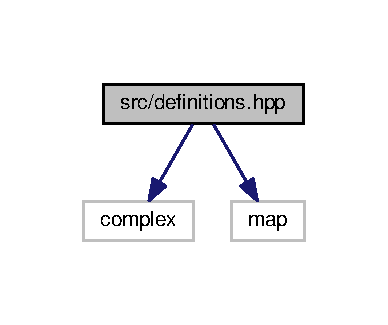
\includegraphics[width=186pt]{definitions_8hpp__incl}
\end{center}
\end{figure}
This graph shows which files directly or indirectly include this file\+:
\nopagebreak
\begin{figure}[H]
\begin{center}
\leavevmode
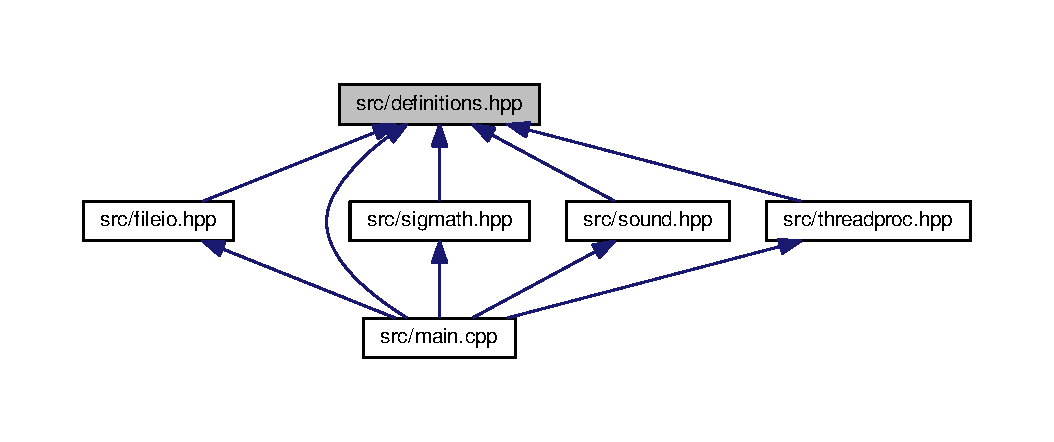
\includegraphics[width=350pt]{definitions_8hpp__dep__incl}
\end{center}
\end{figure}
\subsection*{Classes}
\begin{DoxyCompactItemize}
\item 
struct \hyperlink{structDataParams}{Data\+Params}
\item 
struct \hyperlink{structMaximum}{Maximum}
\item 
struct \hyperlink{structThreadParams}{Thread\+Params}
\end{DoxyCompactItemize}
\subsection*{Namespaces}
\begin{DoxyCompactItemize}
\item 
 \hyperlink{namespacevaso}{vaso}
\begin{DoxyCompactList}\small\item\em contains functions related to the file I/\+O use in this program \end{DoxyCompactList}\end{DoxyCompactItemize}
\subsection*{Macros}
\begin{DoxyCompactItemize}
\item 
\#define \hyperlink{definitions_8hpp_a8fe83ac76edc595f6b98cd4a4127aed5}{E\+R\+R\+O\+R}~-\/1
\begin{DoxyCompactList}\small\item\em Contains declarations of system-\/independant (universal size) integers and float types, shortened type names for some commonly used types, and enumerations. \end{DoxyCompactList}\item 
\#define \hyperlink{definitions_8hpp_aa44e6143be9e89f19be973956c22e134}{R\+E\+C\+\_\+\+C\+O\+U\+N\+T}~8
\item 
\#define \hyperlink{definitions_8hpp_a1682c770d91c5d167b621a782be940d4}{S\+A\+M\+P\+L\+E\+\_\+\+C\+O\+U\+N\+T}~262144
\item 
\#define \hyperlink{definitions_8hpp_a9401e43a8c86acafb31c8e2709baefa1}{S\+A\+M\+P\+L\+E\+\_\+\+F\+R\+E\+Q}~48000
\item 
\#define \hyperlink{definitions_8hpp_a378181c29a641d58f55d647b5a9599f2}{E\+N\+U\+M}~signed char
\end{DoxyCompactItemize}
\subsection*{Typedefs}
\begin{DoxyCompactItemize}
\item 
typedef unsigned char \hyperlink{definitions_8hpp_a0c8186d9b9b7880309c27230bbb5e69d}{byte}
\item 
typedef unsigned char \hyperlink{definitions_8hpp_adde6aaee8457bee49c2a92621fe22b79}{uint8}
\item 
typedef signed char \hyperlink{definitions_8hpp_a1a6408291ee3cfd0760a61ac64084154}{sint8}
\item 
typedef unsigned short \hyperlink{definitions_8hpp_a05f6b0ae8f6a6e135b0e290c25fe0e4e}{uint16}
\item 
typedef signed short \hyperlink{definitions_8hpp_a74df79fde3c518e55b29ce6360a9c76e}{sint16}
\item 
typedef unsigned int \hyperlink{definitions_8hpp_a1134b580f8da4de94ca6b1de4d37975e}{uint32}
\item 
typedef signed int \hyperlink{definitions_8hpp_a0573de65958b4fda3a0460ed417dafb8}{sint32}
\item 
typedef unsigned long long \hyperlink{definitions_8hpp_a29940ae63ec06c9998bba873e25407ad}{uint64}
\item 
typedef signed long long \hyperlink{definitions_8hpp_ad91d7e42d1c1abce1d9eeacd54cc0497}{sint64}
\item 
typedef float \hyperlink{definitions_8hpp_aacdc525d6f7bddb3ae95d5c311bd06a1}{float32}
\item 
typedef double \hyperlink{definitions_8hpp_a232fad1b0d6dcc7c16aabde98b2e2a80}{float64}
\item 
typedef std\+::complex$<$ \hyperlink{definitions_8hpp_aacdc525d6f7bddb3ae95d5c311bd06a1}{float32} $>$ \hyperlink{definitions_8hpp_a960be6b6614c08090c16574dba10a421}{cfloat32}
\end{DoxyCompactItemize}
\subsection*{Enumerations}
\begin{DoxyCompactItemize}
\item 
enum \hyperlink{namespacevaso_a77c5d9704657d49d456f691ddd8abf7c}{vaso\+::\+Side} \{ \hyperlink{namespacevaso_a77c5d9704657d49d456f691ddd8abf7ca945d5e233cf7d6240f6b783b36a374ff}{vaso\+::\+Side\+::\+Left}, 
\hyperlink{namespacevaso_a77c5d9704657d49d456f691ddd8abf7ca92b09c7c48c520c3c55e497875da437c}{vaso\+::\+Side\+::\+Right}
 \}
\end{DoxyCompactItemize}


\subsection{Macro Definition Documentation}
\hypertarget{definitions_8hpp_a378181c29a641d58f55d647b5a9599f2}{\index{definitions.\+hpp@{definitions.\+hpp}!E\+N\+U\+M@{E\+N\+U\+M}}
\index{E\+N\+U\+M@{E\+N\+U\+M}!definitions.\+hpp@{definitions.\+hpp}}
\subsubsection[{E\+N\+U\+M}]{\setlength{\rightskip}{0pt plus 5cm}\#define E\+N\+U\+M~signed char}}\label{definitions_8hpp_a378181c29a641d58f55d647b5a9599f2}


Definition at line \hyperlink{definitions_8hpp_source_l00018}{18} of file \hyperlink{definitions_8hpp_source}{definitions.\+hpp}.

\hypertarget{definitions_8hpp_a8fe83ac76edc595f6b98cd4a4127aed5}{\index{definitions.\+hpp@{definitions.\+hpp}!E\+R\+R\+O\+R@{E\+R\+R\+O\+R}}
\index{E\+R\+R\+O\+R@{E\+R\+R\+O\+R}!definitions.\+hpp@{definitions.\+hpp}}
\subsubsection[{E\+R\+R\+O\+R}]{\setlength{\rightskip}{0pt plus 5cm}\#define E\+R\+R\+O\+R~-\/1}}\label{definitions_8hpp_a8fe83ac76edc595f6b98cd4a4127aed5}


Contains declarations of system-\/independant (universal size) integers and float types, shortened type names for some commonly used types, and enumerations. 

\begin{DoxyAuthor}{Author}
Samuel Andrew Wisner, \href{mailto:awisner94@gmail.com}{\tt awisner94@gmail.\+com} 
\end{DoxyAuthor}


Definition at line \hyperlink{definitions_8hpp_source_l00014}{14} of file \hyperlink{definitions_8hpp_source}{definitions.\+hpp}.

\hypertarget{definitions_8hpp_aa44e6143be9e89f19be973956c22e134}{\index{definitions.\+hpp@{definitions.\+hpp}!R\+E\+C\+\_\+\+C\+O\+U\+N\+T@{R\+E\+C\+\_\+\+C\+O\+U\+N\+T}}
\index{R\+E\+C\+\_\+\+C\+O\+U\+N\+T@{R\+E\+C\+\_\+\+C\+O\+U\+N\+T}!definitions.\+hpp@{definitions.\+hpp}}
\subsubsection[{R\+E\+C\+\_\+\+C\+O\+U\+N\+T}]{\setlength{\rightskip}{0pt plus 5cm}\#define R\+E\+C\+\_\+\+C\+O\+U\+N\+T~8}}\label{definitions_8hpp_aa44e6143be9e89f19be973956c22e134}


Definition at line \hyperlink{definitions_8hpp_source_l00015}{15} of file \hyperlink{definitions_8hpp_source}{definitions.\+hpp}.

\hypertarget{definitions_8hpp_a1682c770d91c5d167b621a782be940d4}{\index{definitions.\+hpp@{definitions.\+hpp}!S\+A\+M\+P\+L\+E\+\_\+\+C\+O\+U\+N\+T@{S\+A\+M\+P\+L\+E\+\_\+\+C\+O\+U\+N\+T}}
\index{S\+A\+M\+P\+L\+E\+\_\+\+C\+O\+U\+N\+T@{S\+A\+M\+P\+L\+E\+\_\+\+C\+O\+U\+N\+T}!definitions.\+hpp@{definitions.\+hpp}}
\subsubsection[{S\+A\+M\+P\+L\+E\+\_\+\+C\+O\+U\+N\+T}]{\setlength{\rightskip}{0pt plus 5cm}\#define S\+A\+M\+P\+L\+E\+\_\+\+C\+O\+U\+N\+T~262144}}\label{definitions_8hpp_a1682c770d91c5d167b621a782be940d4}


Definition at line \hyperlink{definitions_8hpp_source_l00016}{16} of file \hyperlink{definitions_8hpp_source}{definitions.\+hpp}.

\hypertarget{definitions_8hpp_a9401e43a8c86acafb31c8e2709baefa1}{\index{definitions.\+hpp@{definitions.\+hpp}!S\+A\+M\+P\+L\+E\+\_\+\+F\+R\+E\+Q@{S\+A\+M\+P\+L\+E\+\_\+\+F\+R\+E\+Q}}
\index{S\+A\+M\+P\+L\+E\+\_\+\+F\+R\+E\+Q@{S\+A\+M\+P\+L\+E\+\_\+\+F\+R\+E\+Q}!definitions.\+hpp@{definitions.\+hpp}}
\subsubsection[{S\+A\+M\+P\+L\+E\+\_\+\+F\+R\+E\+Q}]{\setlength{\rightskip}{0pt plus 5cm}\#define S\+A\+M\+P\+L\+E\+\_\+\+F\+R\+E\+Q~48000}}\label{definitions_8hpp_a9401e43a8c86acafb31c8e2709baefa1}


Definition at line \hyperlink{definitions_8hpp_source_l00017}{17} of file \hyperlink{definitions_8hpp_source}{definitions.\+hpp}.



\subsection{Typedef Documentation}
\hypertarget{definitions_8hpp_a0c8186d9b9b7880309c27230bbb5e69d}{\index{definitions.\+hpp@{definitions.\+hpp}!byte@{byte}}
\index{byte@{byte}!definitions.\+hpp@{definitions.\+hpp}}
\subsubsection[{byte}]{\setlength{\rightskip}{0pt plus 5cm}typedef unsigned char {\bf byte}}}\label{definitions_8hpp_a0c8186d9b9b7880309c27230bbb5e69d}


Definition at line \hyperlink{definitions_8hpp_source_l00020}{20} of file \hyperlink{definitions_8hpp_source}{definitions.\+hpp}.

\hypertarget{definitions_8hpp_a960be6b6614c08090c16574dba10a421}{\index{definitions.\+hpp@{definitions.\+hpp}!cfloat32@{cfloat32}}
\index{cfloat32@{cfloat32}!definitions.\+hpp@{definitions.\+hpp}}
\subsubsection[{cfloat32}]{\setlength{\rightskip}{0pt plus 5cm}typedef std\+::complex$<${\bf float32}$>$ {\bf cfloat32}}}\label{definitions_8hpp_a960be6b6614c08090c16574dba10a421}
Defines a type for complex float32's. 

Definition at line \hyperlink{definitions_8hpp_source_l00039}{39} of file \hyperlink{definitions_8hpp_source}{definitions.\+hpp}.

\hypertarget{definitions_8hpp_aacdc525d6f7bddb3ae95d5c311bd06a1}{\index{definitions.\+hpp@{definitions.\+hpp}!float32@{float32}}
\index{float32@{float32}!definitions.\+hpp@{definitions.\+hpp}}
\subsubsection[{float32}]{\setlength{\rightskip}{0pt plus 5cm}typedef float {\bf float32}}}\label{definitions_8hpp_aacdc525d6f7bddb3ae95d5c311bd06a1}


Definition at line \hyperlink{definitions_8hpp_source_l00033}{33} of file \hyperlink{definitions_8hpp_source}{definitions.\+hpp}.

\hypertarget{definitions_8hpp_a232fad1b0d6dcc7c16aabde98b2e2a80}{\index{definitions.\+hpp@{definitions.\+hpp}!float64@{float64}}
\index{float64@{float64}!definitions.\+hpp@{definitions.\+hpp}}
\subsubsection[{float64}]{\setlength{\rightskip}{0pt plus 5cm}typedef double {\bf float64}}}\label{definitions_8hpp_a232fad1b0d6dcc7c16aabde98b2e2a80}


Definition at line \hyperlink{definitions_8hpp_source_l00034}{34} of file \hyperlink{definitions_8hpp_source}{definitions.\+hpp}.

\hypertarget{definitions_8hpp_a74df79fde3c518e55b29ce6360a9c76e}{\index{definitions.\+hpp@{definitions.\+hpp}!sint16@{sint16}}
\index{sint16@{sint16}!definitions.\+hpp@{definitions.\+hpp}}
\subsubsection[{sint16}]{\setlength{\rightskip}{0pt plus 5cm}typedef signed short {\bf sint16}}}\label{definitions_8hpp_a74df79fde3c518e55b29ce6360a9c76e}


Definition at line \hyperlink{definitions_8hpp_source_l00025}{25} of file \hyperlink{definitions_8hpp_source}{definitions.\+hpp}.

\hypertarget{definitions_8hpp_a0573de65958b4fda3a0460ed417dafb8}{\index{definitions.\+hpp@{definitions.\+hpp}!sint32@{sint32}}
\index{sint32@{sint32}!definitions.\+hpp@{definitions.\+hpp}}
\subsubsection[{sint32}]{\setlength{\rightskip}{0pt plus 5cm}typedef signed int {\bf sint32}}}\label{definitions_8hpp_a0573de65958b4fda3a0460ed417dafb8}


Definition at line \hyperlink{definitions_8hpp_source_l00028}{28} of file \hyperlink{definitions_8hpp_source}{definitions.\+hpp}.

\hypertarget{definitions_8hpp_ad91d7e42d1c1abce1d9eeacd54cc0497}{\index{definitions.\+hpp@{definitions.\+hpp}!sint64@{sint64}}
\index{sint64@{sint64}!definitions.\+hpp@{definitions.\+hpp}}
\subsubsection[{sint64}]{\setlength{\rightskip}{0pt plus 5cm}typedef signed long long {\bf sint64}}}\label{definitions_8hpp_ad91d7e42d1c1abce1d9eeacd54cc0497}


Definition at line \hyperlink{definitions_8hpp_source_l00031}{31} of file \hyperlink{definitions_8hpp_source}{definitions.\+hpp}.

\hypertarget{definitions_8hpp_a1a6408291ee3cfd0760a61ac64084154}{\index{definitions.\+hpp@{definitions.\+hpp}!sint8@{sint8}}
\index{sint8@{sint8}!definitions.\+hpp@{definitions.\+hpp}}
\subsubsection[{sint8}]{\setlength{\rightskip}{0pt plus 5cm}typedef signed char {\bf sint8}}}\label{definitions_8hpp_a1a6408291ee3cfd0760a61ac64084154}


Definition at line \hyperlink{definitions_8hpp_source_l00022}{22} of file \hyperlink{definitions_8hpp_source}{definitions.\+hpp}.

\hypertarget{definitions_8hpp_a05f6b0ae8f6a6e135b0e290c25fe0e4e}{\index{definitions.\+hpp@{definitions.\+hpp}!uint16@{uint16}}
\index{uint16@{uint16}!definitions.\+hpp@{definitions.\+hpp}}
\subsubsection[{uint16}]{\setlength{\rightskip}{0pt plus 5cm}typedef unsigned short {\bf uint16}}}\label{definitions_8hpp_a05f6b0ae8f6a6e135b0e290c25fe0e4e}


Definition at line \hyperlink{definitions_8hpp_source_l00024}{24} of file \hyperlink{definitions_8hpp_source}{definitions.\+hpp}.

\hypertarget{definitions_8hpp_a1134b580f8da4de94ca6b1de4d37975e}{\index{definitions.\+hpp@{definitions.\+hpp}!uint32@{uint32}}
\index{uint32@{uint32}!definitions.\+hpp@{definitions.\+hpp}}
\subsubsection[{uint32}]{\setlength{\rightskip}{0pt plus 5cm}typedef unsigned int {\bf uint32}}}\label{definitions_8hpp_a1134b580f8da4de94ca6b1de4d37975e}


Definition at line \hyperlink{definitions_8hpp_source_l00027}{27} of file \hyperlink{definitions_8hpp_source}{definitions.\+hpp}.

\hypertarget{definitions_8hpp_a29940ae63ec06c9998bba873e25407ad}{\index{definitions.\+hpp@{definitions.\+hpp}!uint64@{uint64}}
\index{uint64@{uint64}!definitions.\+hpp@{definitions.\+hpp}}
\subsubsection[{uint64}]{\setlength{\rightskip}{0pt plus 5cm}typedef unsigned long long {\bf uint64}}}\label{definitions_8hpp_a29940ae63ec06c9998bba873e25407ad}


Definition at line \hyperlink{definitions_8hpp_source_l00030}{30} of file \hyperlink{definitions_8hpp_source}{definitions.\+hpp}.

\hypertarget{definitions_8hpp_adde6aaee8457bee49c2a92621fe22b79}{\index{definitions.\+hpp@{definitions.\+hpp}!uint8@{uint8}}
\index{uint8@{uint8}!definitions.\+hpp@{definitions.\+hpp}}
\subsubsection[{uint8}]{\setlength{\rightskip}{0pt plus 5cm}typedef unsigned char {\bf uint8}}}\label{definitions_8hpp_adde6aaee8457bee49c2a92621fe22b79}


Definition at line \hyperlink{definitions_8hpp_source_l00021}{21} of file \hyperlink{definitions_8hpp_source}{definitions.\+hpp}.


\hypertarget{definitions_8hpp_source}{\section{definitions.\+hpp}
\label{definitions_8hpp_source}\index{src/definitions.\+hpp@{src/definitions.\+hpp}}
}

\begin{DoxyCode}
00001 
00009 \textcolor{preprocessor}{#ifndef definitions\_H}
00010 \textcolor{preprocessor}{#define definitions\_H}
00011 
00012 \textcolor{preprocessor}{#include <complex>}
00013 \textcolor{preprocessor}{#include <map>}
00014 \textcolor{preprocessor}{#include <string>}
00015 
\hypertarget{definitions_8hpp_source_l00016}{}\hyperlink{definitions_8hpp_a378181c29a641d58f55d647b5a9599f2}{00016} \textcolor{preprocessor}{#define ENUM signed char}
00017 
00018 \textcolor{comment}{// Type definitions}
00019 
\hypertarget{definitions_8hpp_source_l00020}{}\hyperlink{definitions_8hpp_a0c8186d9b9b7880309c27230bbb5e69d}{00020} \textcolor{keyword}{typedef} \textcolor{keywordtype}{unsigned} \textcolor{keywordtype}{char} \hyperlink{definitions_8hpp_a0c8186d9b9b7880309c27230bbb5e69d}{byte};
\hypertarget{definitions_8hpp_source_l00021}{}\hyperlink{definitions_8hpp_adde6aaee8457bee49c2a92621fe22b79}{00021} \textcolor{keyword}{typedef} \textcolor{keywordtype}{unsigned} \textcolor{keywordtype}{char} \hyperlink{definitions_8hpp_adde6aaee8457bee49c2a92621fe22b79}{uint8};
\hypertarget{definitions_8hpp_source_l00022}{}\hyperlink{definitions_8hpp_a1a6408291ee3cfd0760a61ac64084154}{00022} \textcolor{keyword}{typedef} \textcolor{keywordtype}{signed} \textcolor{keywordtype}{char} \hyperlink{definitions_8hpp_a1a6408291ee3cfd0760a61ac64084154}{sint8};
00023 
\hypertarget{definitions_8hpp_source_l00024}{}\hyperlink{definitions_8hpp_a05f6b0ae8f6a6e135b0e290c25fe0e4e}{00024} \textcolor{keyword}{typedef} \textcolor{keywordtype}{unsigned} \textcolor{keywordtype}{short} \hyperlink{definitions_8hpp_a05f6b0ae8f6a6e135b0e290c25fe0e4e}{uint16};
\hypertarget{definitions_8hpp_source_l00025}{}\hyperlink{definitions_8hpp_a74df79fde3c518e55b29ce6360a9c76e}{00025} \textcolor{keyword}{typedef} \textcolor{keywordtype}{signed} \textcolor{keywordtype}{short} \hyperlink{definitions_8hpp_a74df79fde3c518e55b29ce6360a9c76e}{sint16};
00026 
\hypertarget{definitions_8hpp_source_l00027}{}\hyperlink{definitions_8hpp_a1134b580f8da4de94ca6b1de4d37975e}{00027} \textcolor{keyword}{typedef} \textcolor{keywordtype}{unsigned} \textcolor{keywordtype}{int} \hyperlink{definitions_8hpp_a1134b580f8da4de94ca6b1de4d37975e}{uint32};
\hypertarget{definitions_8hpp_source_l00028}{}\hyperlink{definitions_8hpp_a0573de65958b4fda3a0460ed417dafb8}{00028} \textcolor{keyword}{typedef} \textcolor{keywordtype}{signed} \textcolor{keywordtype}{int} \hyperlink{definitions_8hpp_a0573de65958b4fda3a0460ed417dafb8}{sint32};
00029 
\hypertarget{definitions_8hpp_source_l00030}{}\hyperlink{definitions_8hpp_a29940ae63ec06c9998bba873e25407ad}{00030} \textcolor{keyword}{typedef} \textcolor{keywordtype}{unsigned} \textcolor{keywordtype}{long} \textcolor{keywordtype}{long} \hyperlink{definitions_8hpp_a29940ae63ec06c9998bba873e25407ad}{uint64};
\hypertarget{definitions_8hpp_source_l00031}{}\hyperlink{definitions_8hpp_ad91d7e42d1c1abce1d9eeacd54cc0497}{00031} \textcolor{keyword}{typedef} \textcolor{keywordtype}{signed} \textcolor{keywordtype}{long} \textcolor{keywordtype}{long} \hyperlink{definitions_8hpp_ad91d7e42d1c1abce1d9eeacd54cc0497}{sint64};
00032 
\hypertarget{definitions_8hpp_source_l00033}{}\hyperlink{definitions_8hpp_aacdc525d6f7bddb3ae95d5c311bd06a1}{00033} \textcolor{keyword}{typedef} \textcolor{keywordtype}{float} \hyperlink{definitions_8hpp_aacdc525d6f7bddb3ae95d5c311bd06a1}{float32};
\hypertarget{definitions_8hpp_source_l00034}{}\hyperlink{definitions_8hpp_a232fad1b0d6dcc7c16aabde98b2e2a80}{00034} \textcolor{keyword}{typedef} \textcolor{keywordtype}{double} \hyperlink{definitions_8hpp_a232fad1b0d6dcc7c16aabde98b2e2a80}{float64};
00035 
00036 
00037 \textcolor{comment}{// Constants}
00038 
\hypertarget{definitions_8hpp_source_l00042}{}\hyperlink{definitions_8hpp_ac686b5c4edb9968dade15aad6e58bdca}{00042} \textcolor{keyword}{const} std::string \hyperlink{definitions_8hpp_ac686b5c4edb9968dade15aad6e58bdca}{CSV\_HEADER} = \textcolor{stringliteral}{"Time,Side,Frequency,Noise Level"};
00043 
\hypertarget{definitions_8hpp_source_l00048}{}\hyperlink{definitions_8hpp_aa15adfcc96559f1b86210d217edd3afc}{00048} \textcolor{keyword}{const} \hyperlink{definitions_8hpp_a05f6b0ae8f6a6e135b0e290c25fe0e4e}{uint16} \hyperlink{definitions_8hpp_aa15adfcc96559f1b86210d217edd3afc}{DET\_THRESH} = 5000;
00049 
\hypertarget{definitions_8hpp_source_l00053}{}\hyperlink{definitions_8hpp_ada7a88c013312e76596a2000cc8277fb}{00053} \textcolor{keyword}{const} \hyperlink{definitions_8hpp_adde6aaee8457bee49c2a92621fe22b79}{uint8} \hyperlink{definitions_8hpp_ada7a88c013312e76596a2000cc8277fb}{DURATION} = 6;
00054 
\hypertarget{definitions_8hpp_source_l00058}{}\hyperlink{definitions_8hpp_a876fcacb67d51738e846a3312dc08fbb}{00058} \textcolor{keyword}{const} \hyperlink{definitions_8hpp_a1a6408291ee3cfd0760a61ac64084154}{sint8} \hyperlink{definitions_8hpp_a876fcacb67d51738e846a3312dc08fbb}{ERROR} = -1;
00059 
\hypertarget{definitions_8hpp_source_l00063}{}\hyperlink{definitions_8hpp_ab506614aee9be52f401d8d573a8d172c}{00063} \textcolor{keyword}{const} \hyperlink{definitions_8hpp_a05f6b0ae8f6a6e135b0e290c25fe0e4e}{uint16} \hyperlink{definitions_8hpp_ab506614aee9be52f401d8d573a8d172c}{MAX\_DROP\_FREQ} = 7000;
00064 
\hypertarget{definitions_8hpp_source_l00068}{}\hyperlink{definitions_8hpp_a5736990e7ea949fc1971afa00e421f16}{00068} \textcolor{keyword}{const} std::string \hyperlink{definitions_8hpp_a5736990e7ea949fc1971afa00e421f16}{PATIENT\_PATH} = \textcolor{stringliteral}{"/home/pi/patients/"};
00069 
\hypertarget{definitions_8hpp_source_l00073}{}\hyperlink{definitions_8hpp_a2fd18fd694a2918f7d73eba821fd10b2}{00073} \textcolor{keyword}{const} \hyperlink{definitions_8hpp_adde6aaee8457bee49c2a92621fe22b79}{uint8} \hyperlink{definitions_8hpp_a2fd18fd694a2918f7d73eba821fd10b2}{REC\_COUNT} = 6;
00074 
\hypertarget{definitions_8hpp_source_l00079}{}\hyperlink{definitions_8hpp_ad3af99f5e7cbf2af51be580e91faa934}{00079} \textcolor{keyword}{const} \hyperlink{definitions_8hpp_a1134b580f8da4de94ca6b1de4d37975e}{uint32} \hyperlink{definitions_8hpp_ad3af99f5e7cbf2af51be580e91faa934}{SAMPLE\_COUNT} = 131072;\textcolor{comment}{//262144;}
00080 
\hypertarget{definitions_8hpp_source_l00084}{}\hyperlink{definitions_8hpp_a8ace559345ecba7978591ac2ef22aea4}{00084} \textcolor{keyword}{const} \hyperlink{definitions_8hpp_a05f6b0ae8f6a6e135b0e290c25fe0e4e}{uint16} \hyperlink{definitions_8hpp_a8ace559345ecba7978591ac2ef22aea4}{SAMPLE\_FREQ} = 24000;
00085 
\hypertarget{definitions_8hpp_source_l00089}{}\hyperlink{definitions_8hpp_a88f32e97c41b89ff0705d0a0b8566b41}{00089} \textcolor{keyword}{const} std::string \hyperlink{definitions_8hpp_a88f32e97c41b89ff0705d0a0b8566b41}{TEMP\_FILE} = \textcolor{stringliteral}{".temp"};
00090 
\hypertarget{definitions_8hpp_source_l00094}{}\hyperlink{definitions_8hpp_aca681ed285767aaa2353bf3b42dd60ed}{00094} \textcolor{keyword}{const} \hyperlink{definitions_8hpp_a1134b580f8da4de94ca6b1de4d37975e}{uint32} \hyperlink{definitions_8hpp_aca681ed285767aaa2353bf3b42dd60ed}{BUFFER\_SIZE} = \hyperlink{definitions_8hpp_ad3af99f5e7cbf2af51be580e91faa934}{SAMPLE\_COUNT} * \textcolor{keyword}{sizeof}(
      \hyperlink{definitions_8hpp_aacdc525d6f7bddb3ae95d5c311bd06a1}{float32});
00095 
00096 
00097 \textcolor{comment}{// Objective/structural type definitions}
00098 
\hypertarget{definitions_8hpp_source_l00102}{}\hyperlink{definitions_8hpp_a960be6b6614c08090c16574dba10a421}{00102} \textcolor{keyword}{typedef} std::complex<float32> \hyperlink{definitions_8hpp_a960be6b6614c08090c16574dba10a421}{cfloat32};
00103 
\hypertarget{definitions_8hpp_source_l00107}{}\hyperlink{structDataParams}{00107} \textcolor{keyword}{typedef} \textcolor{keyword}{struct }\{
\hypertarget{definitions_8hpp_source_l00111}{}\hyperlink{structDataParams_a12566e017407647bc8287d62554ad3fb}{00111}     \hyperlink{definitions_8hpp_aacdc525d6f7bddb3ae95d5c311bd06a1}{float32} freq = 0;
00112     
\hypertarget{definitions_8hpp_source_l00116}{}\hyperlink{structDataParams_a4efd1d2231c6fa7c878c9d5e1650738f}{00116}     \hyperlink{definitions_8hpp_aacdc525d6f7bddb3ae95d5c311bd06a1}{float32} noise = 0;
00117 \} \hyperlink{structDataParams}{DataParams};
00118 
\hypertarget{definitions_8hpp_source_l00123}{}\hyperlink{structMaximum}{00123} \textcolor{keyword}{typedef} \textcolor{keyword}{struct }\{
\hypertarget{definitions_8hpp_source_l00127}{}\hyperlink{structMaximum_aa7e84cbf37b694670142670014366969}{00127}     \hyperlink{definitions_8hpp_aacdc525d6f7bddb3ae95d5c311bd06a1}{float32} value = 0;
00128     
\hypertarget{definitions_8hpp_source_l00132}{}\hyperlink{structMaximum_a2e6aef03795cd285fe542d0861c6e3b5}{00132}     \hyperlink{definitions_8hpp_a1134b580f8da4de94ca6b1de4d37975e}{uint32} index = 0;
00133 \} \hyperlink{structMaximum}{Maximum};
00134 
00135 
00136 \textcolor{comment}{// Enumerations}
00137 
\hypertarget{definitions_8hpp_source_l00141}{}\hyperlink{namespaceavda}{00141} \textcolor{keyword}{namespace }\hyperlink{namespaceavda}{avda} \{
\hypertarget{definitions_8hpp_source_l00145}{}\hyperlink{namespaceavda_af723e82f0d3d45fda6fdc01f6a492786}{00145}     \textcolor{keyword}{enum class} \hyperlink{namespaceavda_af723e82f0d3d45fda6fdc01f6a492786}{Side} \{ \hyperlink{namespaceavda_af723e82f0d3d45fda6fdc01f6a492786a945d5e233cf7d6240f6b783b36a374ff}{Left}, \hyperlink{namespaceavda_af723e82f0d3d45fda6fdc01f6a492786a92b09c7c48c520c3c55e497875da437c}{Right} \};
00146 \}
00147 
00148 
00149 \textcolor{comment}{// Doxygen documentation for other files.}
00150 
00171 \textcolor{preprocessor}{#endif}
\end{DoxyCode}

\hypertarget{fileio_8hpp}{\section{src/fileio.hpp File Reference}
\label{fileio_8hpp}\index{src/fileio.\+hpp@{src/fileio.\+hpp}}
}


contains functions related to the file I/\+O use in this program  


{\ttfamily \#include $<$fstream$>$}\\*
{\ttfamily \#include $<$iostream$>$}\\*
{\ttfamily \#include $<$sstream$>$}\\*
{\ttfamily \#include $<$string$>$}\\*
{\ttfamily \#include $<$stdexcept$>$}\\*
{\ttfamily \#include $<$time.\+h$>$}\\*
{\ttfamily \#include \char`\"{}definitions.\+hpp\char`\"{}}\\*
Include dependency graph for fileio.\+hpp\+:
\nopagebreak
\begin{figure}[H]
\begin{center}
\leavevmode
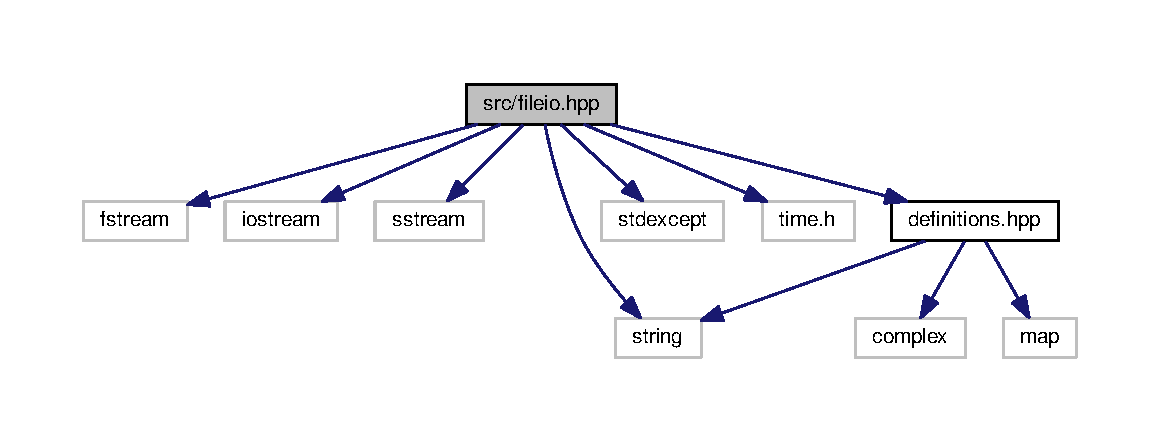
\includegraphics[width=350pt]{fileio_8hpp__incl}
\end{center}
\end{figure}
This graph shows which files directly or indirectly include this file\+:
\nopagebreak
\begin{figure}[H]
\begin{center}
\leavevmode
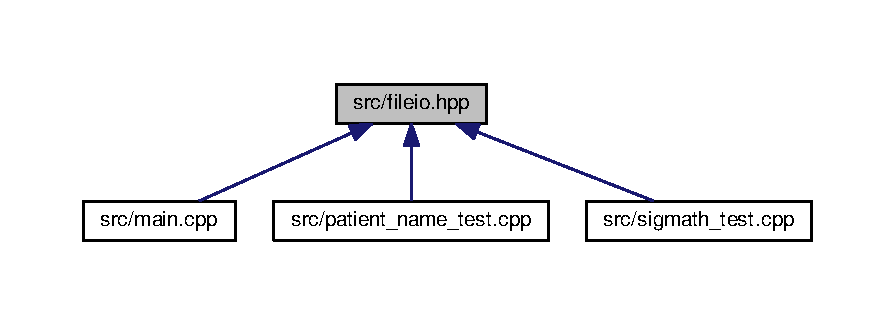
\includegraphics[width=350pt]{fileio_8hpp__dep__incl}
\end{center}
\end{figure}
\subsection*{Namespaces}
\begin{DoxyCompactItemize}
\item 
 \hyperlink{namespaceavda}{avda}
\end{DoxyCompactItemize}
\subsection*{Functions}
\begin{DoxyCompactItemize}
\item 
std\+::string \hyperlink{namespaceavda_ae20728e7e8ae50bf2f74849e538841ea}{avda\+::\+Patient\+Name} ()
\item 
std\+::map$<$ Side, \hyperlink{structDataParams}{Data\+Params} $>$ \hyperlink{namespaceavda_a46dc980b65ddfc24749ce25c1290e158}{avda\+::\+Read\+Params} (auto filename)
\item 
void \hyperlink{namespaceavda_aba04a08b41833ced32ec803d55a63bee}{avda\+::\+Write\+Params} (std\+::map$<$ Side, \hyperlink{structDataParams}{Data\+Params} $>$ my\+Map, auto filename)
\end{DoxyCompactItemize}
\subsection*{Variables}
\begin{DoxyCompactItemize}
\item 
const std\+::string \hyperlink{namespaceavda_ac568a0872c2c176d874b8b12f67f43ea}{avda\+::\+C\+S\+V\+\_\+\+H\+E\+A\+D\+E\+R} = \char`\"{}Time,Side,Frequency,Noise Level\char`\"{}
\item 
const std\+::string \hyperlink{namespaceavda_a8ee73ec0cb55d4a13e89949764dce89d}{avda\+::\+P\+A\+T\+I\+E\+N\+T\+\_\+\+P\+A\+T\+H} = \char`\"{}/home/pi/patients/\char`\"{}
\end{DoxyCompactItemize}


\subsection{Detailed Description}
contains functions related to the file I/\+O use in this program 

\begin{DoxyAuthor}{Author}
Samuel Andrew Wisner, \href{mailto:awisner94@gmail.com}{\tt awisner94@gmail.\+com} 

Nicholas K. Nolan 
\end{DoxyAuthor}
\begin{DoxyRefDesc}{Bug}
\item[\hyperlink{bug__bug000001}{Bug}]file is overly complicated and much more bug-\/prone \end{DoxyRefDesc}


Definition in file \hyperlink{fileio_8hpp_source}{fileio.\+hpp}.


\hypertarget{fileio_8hpp_source}{\section{fileio.\+hpp}
\label{fileio_8hpp_source}\index{src/fileio.\+hpp@{src/fileio.\+hpp}}
}

\begin{DoxyCode}
00001 
00009 \textcolor{preprocessor}{#ifndef fileio\_H}
00010 \textcolor{preprocessor}{#define fileio\_H}
00011 
00012 \textcolor{preprocessor}{#include <fstream>}
00013 \textcolor{preprocessor}{#include <iostream>}
00014 \textcolor{preprocessor}{#include <sstream>}
00015 \textcolor{preprocessor}{#include <string>}
00016 \textcolor{preprocessor}{#include <stdexcept>}
00017 \textcolor{preprocessor}{#include <time.h>}
00018 
00019 \textcolor{preprocessor}{#include "\hyperlink{definitions_8hpp}{definitions.hpp}"}
00020 
00021 \textcolor{keyword}{namespace }\hyperlink{namespaceavda}{avda} \{
\hypertarget{fileio_8hpp_source_l00025}{}\hyperlink{namespaceavda_ac568a0872c2c176d874b8b12f67f43ea}{00025}     \textcolor{keyword}{const} std::string \hyperlink{namespaceavda_ac568a0872c2c176d874b8b12f67f43ea}{CSV\_HEADER} = \textcolor{stringliteral}{"Time,Side,Frequency,Noise Level"};
00026 
\hypertarget{fileio_8hpp_source_l00030}{}\hyperlink{namespaceavda_a8ee73ec0cb55d4a13e89949764dce89d}{00030}     \textcolor{keyword}{const} std::string \hyperlink{namespaceavda_a8ee73ec0cb55d4a13e89949764dce89d}{PATIENT\_PATH} = \textcolor{stringliteral}{"/home/pi/patients/"};
00031 
\hypertarget{fileio_8hpp_source_l00043}{}\hyperlink{namespaceavda_ae20728e7e8ae50bf2f74849e538841ea}{00043}     std::string \hyperlink{namespaceavda_ae20728e7e8ae50bf2f74849e538841ea}{PatientName}() \{
00044         std::string fname = \textcolor{stringliteral}{""};
00045         std::string mname = \textcolor{stringliteral}{""};
00046         std::string lname = \textcolor{stringliteral}{""};
00047         std::string patfil = \textcolor{stringliteral}{""};
00048         std::string patientname = \textcolor{stringliteral}{""};
00049         \hyperlink{definitions_8hpp_a1134b580f8da4de94ca6b1de4d37975e}{uint32} track1 = 0;
00050         \hyperlink{definitions_8hpp_a1134b580f8da4de94ca6b1de4d37975e}{uint32} track2 = 0;
00051         \hyperlink{definitions_8hpp_a1134b580f8da4de94ca6b1de4d37975e}{uint32} track3 = 0;
00052 
00053         \textcolor{keywordflow}{do} \{
00054             std::cout << \textcolor{stringliteral}{"Please enter the patients name."} << std::endl;
00055             std::cout << \textcolor{stringliteral}{"First name: "};
00056             std::cin >> fname;
00057             std::cout << \textcolor{stringliteral}{"Middle name: "};
00058             std::cin >> mname;
00059             std::cout << \textcolor{stringliteral}{"Last name: "};
00060             std::cin >> lname;
00061 
00062             \textcolor{comment}{// creates new std::string with path to patient file}
00063             patientname = PATIENT\_PATH + lname + \textcolor{stringliteral}{", "} + fname
00064                 + \textcolor{stringliteral}{" "} + mname + \textcolor{stringliteral}{".csv"};
00065 
00066             \textcolor{comment}{// prints out patientname. shows user the path to the patient file}
00067             \textcolor{comment}{//std::cout << patientname << std::endl << std::endl;}
00068             std::ifstream file(patientname.c\_str());
00069 
00070             \textcolor{keywordflow}{if} (file.good()) \{
00071                 track1 = 1;
00072             \}
00073 
00074             \textcolor{comment}{/*}
00075 \textcolor{comment}{             * Compares patientname to existing files and lets user know}
00076 \textcolor{comment}{             * if the file does not exist.}
00077 \textcolor{comment}{             */}
00078             \textcolor{keywordflow}{else} \textcolor{keywordflow}{if} (!file.good()) \{
00079                 \textcolor{comment}{/* }
00080 \textcolor{comment}{                 * Do while statement to continue asking user about the file}
00081 \textcolor{comment}{                 * if their input is not acceptable}
00082 \textcolor{comment}{                 */} 
00083                 \textcolor{keywordflow}{do} \{
00084                     std::cout << \textcolor{stringliteral}{"Patient file does not exist, would you like "}
00085                         \textcolor{stringliteral}{"to create file or re-enter their name?"} << std::endl;
00086                     std::cout << \textcolor{stringliteral}{"  *Type 'create' and press enter key "}
00087                         \textcolor{stringliteral}{"to create the patient file."} << std::endl;
00088                     std::cout << \textcolor{stringliteral}{"  *Type 'reenter' and press enter key "}
00089                         \textcolor{stringliteral}{"to re-enter the patients name."} << std::endl;
00090                     std::cout << std::endl;
00091                     std::cin >> patfil;
00092 
00093                     \textcolor{comment}{/* }
00094 \textcolor{comment}{                     * patfil equals create, track1 and 2 will increase}
00095 \textcolor{comment}{                     * escaping both do while loops}
00096 \textcolor{comment}{                     */}
00097                     \textcolor{keywordflow}{if}(patfil == \textcolor{stringliteral}{"create"}) \{
00098                         std::ofstream createfile(patientname.c\_str());
00099                         track1 = 1;
00100                         track2 = 1;
00101                         track3 = 1;
00102                         createfile << CSV\_HEADER << std::endl;
00103                         createfile.flush();
00104                         createfile.close();
00105                     \}
00106 
00107                     \textcolor{comment}{/*}
00108 \textcolor{comment}{                     *patfil equals renter, track1 will remain zero allowing}
00109 \textcolor{comment}{                     *user to reenter the patient name.}
00110 \textcolor{comment}{                     */}
00111                     \textcolor{keywordflow}{else} \textcolor{keywordflow}{if}(patfil == \textcolor{stringliteral}{"reenter"}) \{
00112                         track1 = 0;
00113                         track2 = 1;
00114                     \}
00115 
00116                     \textcolor{comment}{/*}
00117 \textcolor{comment}{                     *The users input was neither create or reenter. User}
00118 \textcolor{comment}{                     *must enter patient name again.}
00119 \textcolor{comment}{                     */}
00120                     \textcolor{keywordflow}{else} \{
00121                         std::cout << std::endl;
00122                         std::cout << \textcolor{stringliteral}{"Your input is not acceptable."} << std::endl;
00123                         std::cout << std::endl;
00124                     \}
00125                 \}\textcolor{keywordflow}{while}(track2 == 0);
00126             \}
00127         \} \textcolor{keywordflow}{while} (track1 == 0);
00128 
00129         \textcolor{keywordflow}{return} patientname; \textcolor{comment}{//returns the path to the patient file}
00130     \}
00131 
\hypertarget{fileio_8hpp_source_l00141}{}\hyperlink{namespaceavda_a46dc980b65ddfc24749ce25c1290e158}{00141}     std::map<Side, DataParams> \hyperlink{namespaceavda_a46dc980b65ddfc24749ce25c1290e158}{ReadParams}(\textcolor{keyword}{auto} filename) \{
00142         std::map<Side, DataParams> myMap;
00143         \hyperlink{structDataParams}{DataParams} leftparams;
00144         \hyperlink{structDataParams}{DataParams} rightparams;
00145 
00146         std::ifstream file(filename.c\_str());
00147         std::string leftline;
00148         std::string rightline;
00149         std::string leftsearch = \textcolor{stringliteral}{"Left"};
00150         std::string rightsearch = \textcolor{stringliteral}{"Right"};
00151         std::string paramstring;
00152         std::string lfreqstr;
00153         std::string lnoisestr;
00154         std::string rfreqstr;
00155         std::string rnoisestr;
00156         \hyperlink{definitions_8hpp_a1134b580f8da4de94ca6b1de4d37975e}{uint32} lcnt = 0;
00157         \hyperlink{definitions_8hpp_a1134b580f8da4de94ca6b1de4d37975e}{uint32} rcnt = 0;
00158         \hyperlink{definitions_8hpp_aacdc525d6f7bddb3ae95d5c311bd06a1}{float32} lfreqval;
00159         \hyperlink{definitions_8hpp_aacdc525d6f7bddb3ae95d5c311bd06a1}{float32} lnoiseval;
00160         \hyperlink{definitions_8hpp_aacdc525d6f7bddb3ae95d5c311bd06a1}{float32} rfreqval;
00161         \hyperlink{definitions_8hpp_aacdc525d6f7bddb3ae95d5c311bd06a1}{float32} rnoiseval;
00162 
00163         \textcolor{comment}{/*}
00164 \textcolor{comment}{         * if statement which uses ifstream function to open patient file }
00165 \textcolor{comment}{         * filename)}
00166 \textcolor{comment}{         */}
00167         \textcolor{keywordflow}{if}(file.is\_open()) \{
00168             \textcolor{comment}{/*}
00169 \textcolor{comment}{             * While statement to find the first Left line and save to }
00170 \textcolor{comment}{             *leftline as string.}
00171 \textcolor{comment}{             */}
00172             \textcolor{keywordflow}{while} (getline(file, leftline)) \{
00173                 \textcolor{keywordflow}{if}(leftline.find(leftsearch, 0) != std::string::npos) \{
00174                     \textcolor{keywordflow}{break};
00175                 \}
00176 
00177             \}
00178 
00179             \textcolor{comment}{/*}
00180 \textcolor{comment}{             * While statement to find first right line and save to rightline}
00181 \textcolor{comment}{             * as string.}
00182 \textcolor{comment}{             */}
00183             \textcolor{keywordflow}{while} (getline(file,rightline)) \{
00184                 \textcolor{keywordflow}{if}(rightline.find(rightsearch, 0) != std::string::npos) \{
00185                     \textcolor{keywordflow}{break};
00186                 \}
00187             \}
00188 
00189             \textcolor{comment}{// Code to break leftline and rightline into its parts}
00190             std::stringstream lss(leftline);
00191             std::stringstream rss(rightline);
00192 
00193             \textcolor{keywordflow}{while}(getline(lss,paramstring, \textcolor{charliteral}{','})) \{
00194                 lcnt++;
00195 
00196                 \textcolor{keywordflow}{if}(lcnt == 3) \{
00197                     lfreqstr = paramstring;
00198                 \}
00199 
00200                 \textcolor{keywordflow}{else} \textcolor{keywordflow}{if}(lcnt == 4) \{
00201                     lnoisestr = paramstring;
00202                 \}
00203             \}
00204 
00205             \textcolor{keywordflow}{while}(getline(rss,paramstring, \textcolor{charliteral}{','})) \{
00206                 rcnt++;
00207 
00208                 \textcolor{keywordflow}{if}(rcnt == 3) \{
00209                     rfreqstr = paramstring;
00210                 \}
00211 
00212                 \textcolor{keywordflow}{else} \textcolor{keywordflow}{if}(rcnt == 4) \{
00213                     rnoisestr = paramstring;
00214                 \}
00215             \}
00216 
00217             \textcolor{comment}{/*}
00218 \textcolor{comment}{             * Statement to convert lfreq, lnoise, rfreq, and rnoise from}
00219 \textcolor{comment}{             * strings to floats.}
00220 \textcolor{comment}{             * */}
00221             lfreqval = atof(lfreqstr.c\_str());
00222             lnoiseval = atof(lnoisestr.c\_str());
00223             rfreqval = atof(rfreqstr.c\_str());
00224             rnoiseval = atof(rnoisestr.c\_str());
00225 
00226             file.close();
00227         \}
00228 
00229         \textcolor{keywordflow}{else} \{
00230             \textcolor{keywordflow}{throw} std::runtime\_error(\textcolor{stringliteral}{"The patient file could not be opened."});
00231         \}
00232 
00233         leftparams.\hyperlink{structDataParams_a12566e017407647bc8287d62554ad3fb}{freq} = lfreqval;
00234         leftparams.\hyperlink{structDataParams_a4efd1d2231c6fa7c878c9d5e1650738f}{noise} = lnoiseval;
00235         rightparams.\hyperlink{structDataParams_a12566e017407647bc8287d62554ad3fb}{freq} = rfreqval;
00236         rightparams.\hyperlink{structDataParams_a4efd1d2231c6fa7c878c9d5e1650738f}{noise} = rnoiseval;
00237 
00238         myMap[\hyperlink{namespaceavda_af723e82f0d3d45fda6fdc01f6a492786a945d5e233cf7d6240f6b783b36a374ff}{Side::Left}] = leftparams;
00239         myMap[\hyperlink{namespaceavda_af723e82f0d3d45fda6fdc01f6a492786a92b09c7c48c520c3c55e497875da437c}{Side::Right}] = rightparams;
00240 
00241         \textcolor{keywordflow}{return} myMap;
00242     \}
00243 
\hypertarget{fileio_8hpp_source_l00251}{}\hyperlink{namespaceavda_aba04a08b41833ced32ec803d55a63bee}{00251}     \textcolor{keywordtype}{void} \hyperlink{namespaceavda_aba04a08b41833ced32ec803d55a63bee}{WriteParams}(std::map<Side, DataParams> myMap, \textcolor{keyword}{auto} filename) \{
00252         \textcolor{keywordtype}{char} temp[80];
00253         std::ofstream file(filename.c\_str(),
00254                 std::ofstream::out | std::ofstream::app);
00255 
00256         \textcolor{comment}{//Gives pointer measurementtime a data type of time\_t.}
00257         time\_t measurementtime;
00258         time(&measurementtime); \textcolor{comment}{//Gets the current time.}
00259         strftime(temp, 80, \textcolor{stringliteral}{"%c"}, localtime(&measurementtime));
00260         std::string fTime = std::string(temp);
00261 
00262         \textcolor{comment}{//if statement to print the Left side parameters to the patient file.}
00263         \textcolor{keywordflow}{if}(file.is\_open()) \{
00264             file << fTime + \textcolor{stringliteral}{","} + \textcolor{stringliteral}{"Left"} + \textcolor{stringliteral}{","}
00265                 + std::to\_string(myMap[\hyperlink{namespaceavda_af723e82f0d3d45fda6fdc01f6a492786a945d5e233cf7d6240f6b783b36a374ff}{Side::Left}].freq) 
00266                 + \textcolor{stringliteral}{", "} + std::to\_string(myMap[\hyperlink{namespaceavda_af723e82f0d3d45fda6fdc01f6a492786a945d5e233cf7d6240f6b783b36a374ff}{Side::Left}].noise) << std::endl;
00267         \}
00268 
00269         \textcolor{comment}{//if statement to print the Right side parameters to the patient file.}
00270         \textcolor{keywordflow}{if}(file.is\_open()) \{
00271             file << fTime + \textcolor{stringliteral}{","} + \textcolor{stringliteral}{"Right"} + \textcolor{stringliteral}{","}
00272                 + std::to\_string(myMap[\hyperlink{namespaceavda_af723e82f0d3d45fda6fdc01f6a492786a92b09c7c48c520c3c55e497875da437c}{Side::Right}].freq) 
00273                 + \textcolor{stringliteral}{", "} + std::to\_string(myMap[\hyperlink{namespaceavda_af723e82f0d3d45fda6fdc01f6a492786a92b09c7c48c520c3c55e497875da437c}{Side::Right}].noise) << std::endl;
00274         \}
00275 
00276         \textcolor{keywordflow}{else} \{
00277             std::cout << \textcolor{stringliteral}{"Patient file can not be opened!"} << std::endl;
00278         \}
00279 
00280         file.close();
00281     \}
00282 \}
00283 
00284 \textcolor{preprocessor}{#endif}
\end{DoxyCode}

\hypertarget{fileio__test_8cpp}{\section{src/fileio\+\_\+test.cpp File Reference}
\label{fileio__test_8cpp}\index{src/fileio\+\_\+test.\+cpp@{src/fileio\+\_\+test.\+cpp}}
}


Contains program that tests the functions in \hyperlink{fileio_8hpp}{fileio.\+hpp}.  


{\ttfamily \#include $<$fstream$>$}\\*
{\ttfamily \#include $<$iostream$>$}\\*
{\ttfamily \#include $<$sstream$>$}\\*
{\ttfamily \#include $<$string$>$}\\*
{\ttfamily \#include $<$time.\+h$>$}\\*
{\ttfamily \#include \char`\"{}definitions.\+hpp\char`\"{}}\\*
{\ttfamily \#include \char`\"{}fileio.\+hpp\char`\"{}}\\*
{\ttfamily \#include \char`\"{}process.\+hpp\char`\"{}}\\*
Include dependency graph for fileio\+\_\+test.\+cpp\+:
\nopagebreak
\begin{figure}[H]
\begin{center}
\leavevmode
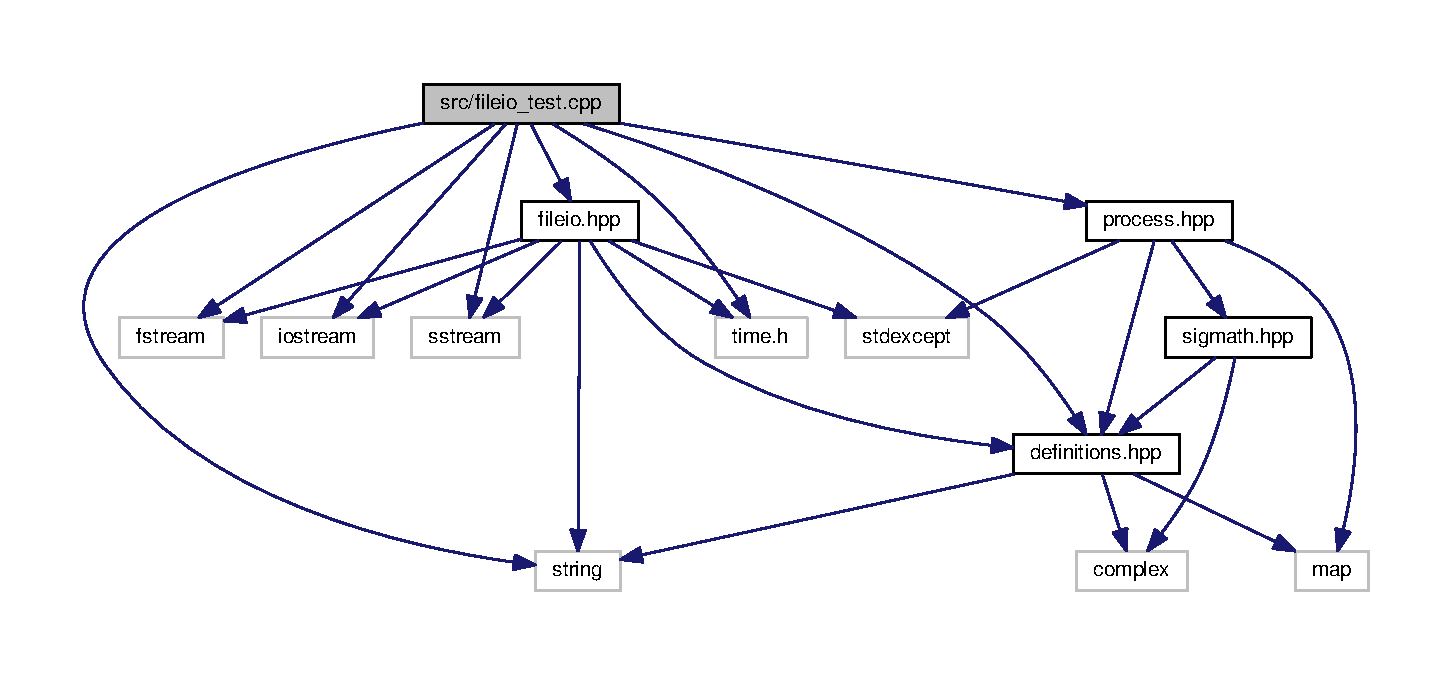
\includegraphics[width=350pt]{fileio__test_8cpp__incl}
\end{center}
\end{figure}
\subsection*{Functions}
\begin{DoxyCompactItemize}
\item 
int \hyperlink{fileio__test_8cpp_ae66f6b31b5ad750f1fe042a706a4e3d4}{main} ()
\end{DoxyCompactItemize}


\subsection{Detailed Description}
Contains program that tests the functions in \hyperlink{fileio_8hpp}{fileio.\+hpp}. 

\begin{DoxyAuthor}{Author}
Samuel Andrew Wisner 

Nicholas K. Nolan 
\end{DoxyAuthor}


Definition in file \hyperlink{fileio__test_8cpp_source}{fileio\+\_\+test.\+cpp}.



\subsection{Function Documentation}
\hypertarget{fileio__test_8cpp_ae66f6b31b5ad750f1fe042a706a4e3d4}{\index{fileio\+\_\+test.\+cpp@{fileio\+\_\+test.\+cpp}!main@{main}}
\index{main@{main}!fileio\+\_\+test.\+cpp@{fileio\+\_\+test.\+cpp}}
\subsubsection[{main}]{\setlength{\rightskip}{0pt plus 5cm}int main (
\begin{DoxyParamCaption}
{}
\end{DoxyParamCaption}
)}}\label{fileio__test_8cpp_ae66f6b31b5ad750f1fe042a706a4e3d4}
Tests the functions in \hyperlink{fileio_8hpp}{fileio.\+hpp}. 

Definition at line \hyperlink{fileio__test_8cpp_source_l00024}{24} of file \hyperlink{fileio__test_8cpp_source}{fileio\+\_\+test.\+cpp}.


\begin{DoxyCode}
00024            \{
00025     \textcolor{keywordtype}{string} path = \hyperlink{namespacevaso_a0f49c8240a13e7d853912ad78d5f53c9}{PATIENT\_PATH} + \textcolor{stringliteral}{"wizmack, sammy andy.csv"};
00026     map<Side, DataParams> laMap = \hyperlink{namespacevaso_afc1435dcb9c37b3ccde589738b26c909}{ReadParams}(path);
00027     cout <<  laMap[Side::Right].freq << endl;
00028     cout << laMap[Side::Right].noise << endl;
00029 
00030     \hyperlink{namespacevaso_ac272f5c7d73f350442d4657ef0258021}{WriteParams}(laMap, path);
00031 \}
\end{DoxyCode}


Here is the call graph for this function\+:
\nopagebreak
\begin{figure}[H]
\begin{center}
\leavevmode
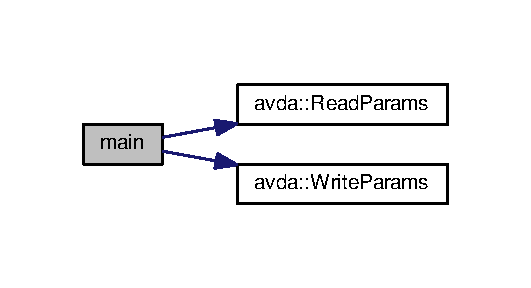
\includegraphics[width=255pt]{fileio__test_8cpp_ae66f6b31b5ad750f1fe042a706a4e3d4_cgraph}
\end{center}
\end{figure}



\hypertarget{fileio__test_8cpp_source}{\section{fileio\+\_\+test.\+cpp}
\label{fileio__test_8cpp_source}\index{src/fileio\+\_\+test.\+cpp@{src/fileio\+\_\+test.\+cpp}}
}

\begin{DoxyCode}
00001 
00008 \textcolor{preprocessor}{#include <fstream>}
00009 \textcolor{preprocessor}{#include <iostream>}
00010 \textcolor{preprocessor}{#include <sstream>}
00011 \textcolor{preprocessor}{#include <string>}
00012 \textcolor{preprocessor}{#include <time.h>}
00013 
00014 \textcolor{preprocessor}{#include "\hyperlink{definitions_8hpp}{definitions.hpp}"}
00015 \textcolor{preprocessor}{#include "\hyperlink{fileio_8hpp}{fileio.hpp}"}
00016 \textcolor{preprocessor}{#include "\hyperlink{process_8hpp}{process.hpp}"}
00017 
00018 \textcolor{keyword}{using namespace }\hyperlink{namespacestd}{std};
00019 \textcolor{keyword}{using namespace }\hyperlink{namespaceavda}{avda};
00020 
\hypertarget{fileio__test_8cpp_source_l00024}{}\hyperlink{fileio__test_8cpp_ae66f6b31b5ad750f1fe042a706a4e3d4}{00024} \textcolor{keywordtype}{int} \hyperlink{fileio__test_8cpp_ae66f6b31b5ad750f1fe042a706a4e3d4}{main}() \{
00025     \textcolor{keywordtype}{string} path = \hyperlink{namespaceavda_a8ee73ec0cb55d4a13e89949764dce89d}{PATIENT\_PATH} + \textcolor{stringliteral}{"wizmack, sammy andy.csv"};
00026     map<Side, DataParams> laMap = \hyperlink{namespaceavda_a46dc980b65ddfc24749ce25c1290e158}{ReadParams}(path);
00027     cout <<  laMap[Side::Right].freq << endl;
00028     cout << laMap[Side::Right].noise << endl;
00029 
00030     \hyperlink{namespaceavda_aba04a08b41833ced32ec803d55a63bee}{WriteParams}(laMap, path);
00031 \}
\end{DoxyCode}

\hypertarget{main_8cpp}{\section{src/main.cpp File Reference}
\label{main_8cpp}\index{src/main.\+cpp@{src/main.\+cpp}}
}
{\ttfamily \#include $<$array$>$}\\*
{\ttfamily \#include $<$cstdlib$>$}\\*
{\ttfamily \#include $<$iostream$>$}\\*
{\ttfamily \#include $<$map$>$}\\*
{\ttfamily \#include $<$pthread.\+h$>$}\\*
{\ttfamily \#include $<$string$>$}\\*
{\ttfamily \#include $<$unistd.\+h$>$}\\*
{\ttfamily \#include \char`\"{}definitions.\+hpp\char`\"{}}\\*
{\ttfamily \#include \char`\"{}fileio.\+hpp\char`\"{}}\\*
{\ttfamily \#include \char`\"{}process.\+hpp\char`\"{}}\\*
Include dependency graph for main.\+cpp\+:
\nopagebreak
\begin{figure}[H]
\begin{center}
\leavevmode
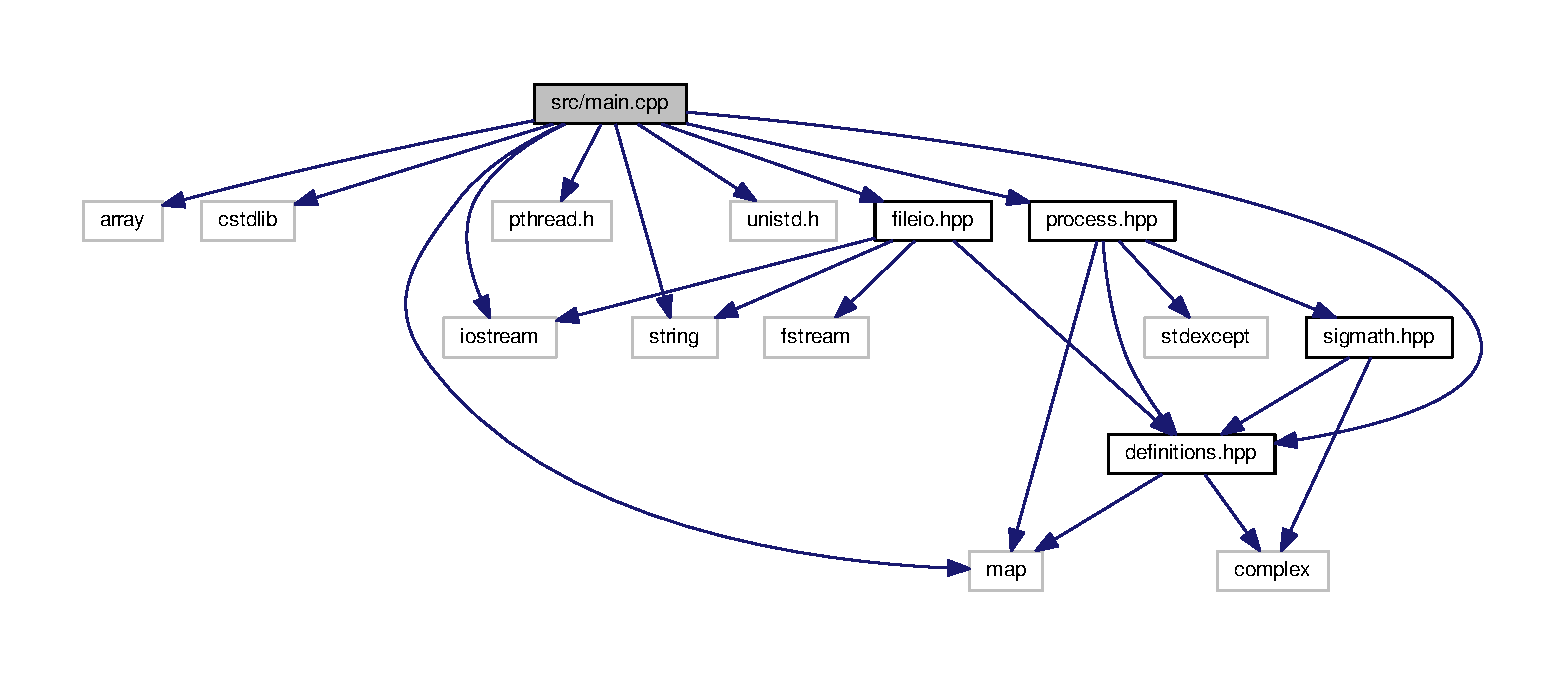
\includegraphics[width=350pt]{main_8cpp__incl}
\end{center}
\end{figure}
\subsection*{Functions}
\begin{DoxyCompactItemize}
\item 
int \hyperlink{main_8cpp_a3c04138a5bfe5d72780bb7e82a18e627}{main} (int argc, char $\ast$$\ast$argv)
\end{DoxyCompactItemize}


\subsection{Function Documentation}
\hypertarget{main_8cpp_a3c04138a5bfe5d72780bb7e82a18e627}{\index{main.\+cpp@{main.\+cpp}!main@{main}}
\index{main@{main}!main.\+cpp@{main.\+cpp}}
\subsubsection[{main}]{\setlength{\rightskip}{0pt plus 5cm}int main (
\begin{DoxyParamCaption}
\item[{int}]{argc, }
\item[{char $\ast$$\ast$}]{argv}
\end{DoxyParamCaption}
)}}\label{main_8cpp_a3c04138a5bfe5d72780bb7e82a18e627}
The main program for this progject. It will detect vasospasms over a period of days. 

Definition at line \hyperlink{main_8cpp_source_l00026}{26} of file \hyperlink{main_8cpp_source}{main.\+cpp}.



Here is the call graph for this function\+:
\nopagebreak
\begin{figure}[H]
\begin{center}
\leavevmode
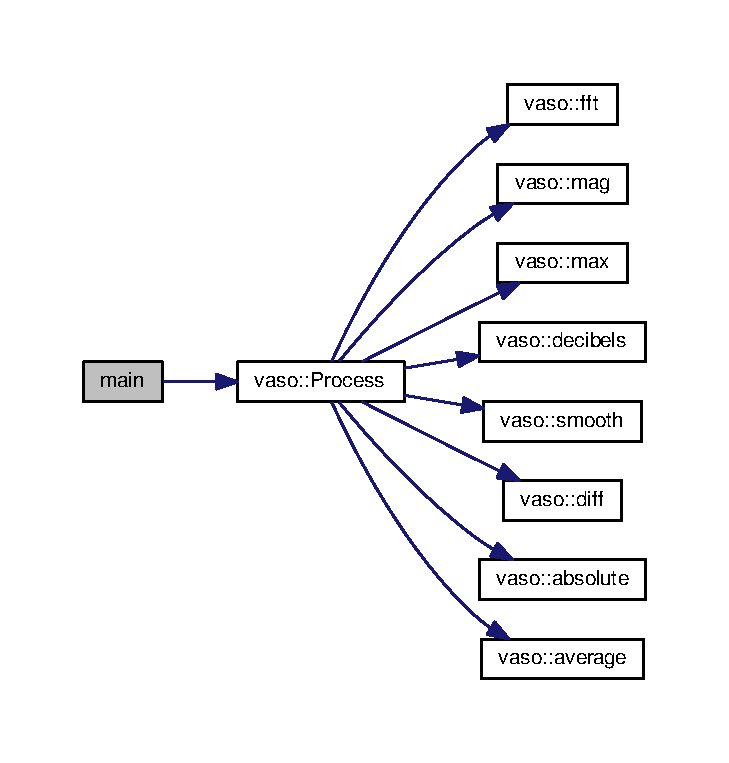
\includegraphics[width=350pt]{main_8cpp_a3c04138a5bfe5d72780bb7e82a18e627_cgraph}
\end{center}
\end{figure}



\hypertarget{main_8cpp_source}{\section{main.\+cpp}
\label{main_8cpp_source}\index{src/main.\+cpp@{src/main.\+cpp}}
}

\begin{DoxyCode}
00001 
00010 \textcolor{preprocessor}{#include <array>}
00011 \textcolor{preprocessor}{#include <cstdio>}
00012 \textcolor{preprocessor}{#include <cstdlib>}
00013 \textcolor{preprocessor}{#include <fcntl.h>}
00014 \textcolor{preprocessor}{#include <iostream>}
00015 \textcolor{preprocessor}{#include <map>}
00016 \textcolor{preprocessor}{#include <pthread.h>}
00017 \textcolor{preprocessor}{#include <string>}
00018 \textcolor{preprocessor}{#include <unistd.h>}
00019 
00020 \textcolor{preprocessor}{#include "\hyperlink{definitions_8hpp}{definitions.hpp}"}
00021 \textcolor{preprocessor}{#include "\hyperlink{fileio_8hpp}{fileio.hpp}"}
00022 \textcolor{preprocessor}{#include "\hyperlink{process_8hpp}{process.hpp}"}
00023 
00024 \textcolor{keyword}{using namespace }\hyperlink{namespacestd}{std};
00025 \textcolor{keyword}{using namespace }\hyperlink{namespaceavda}{avda};
00026 
\hypertarget{main_8cpp_source_l00031}{}\hyperlink{main_8cpp_a3c04138a5bfe5d72780bb7e82a18e627}{00031} \textcolor{keywordtype}{int} \hyperlink{main_8cpp_a3c04138a5bfe5d72780bb7e82a18e627}{main}(\textcolor{keywordtype}{int} argc, \textcolor{keywordtype}{char}** argv) \{
00032     \textcolor{comment}{// Recorded audio buffer}
00033     \hyperlink{definitions_8hpp_aacdc525d6f7bddb3ae95d5c311bd06a1}{float32}* buffer = (\hyperlink{definitions_8hpp_aacdc525d6f7bddb3ae95d5c311bd06a1}{float32}*)std::malloc(\hyperlink{definitions_8hpp_aca681ed285767aaa2353bf3b42dd60ed}{BUFFER\_SIZE});
00034     \textcolor{keywordtype}{bool} cont = \textcolor{keyword}{true};  \textcolor{comment}{// whether to continue in the recording loop}
00035     \hyperlink{structDataParams}{DataParams} params[\hyperlink{definitions_8hpp_a2fd18fd694a2918f7d73eba821fd10b2}{REC\_COUNT}];  \textcolor{comment}{// holds DataParam's from recordings}
00036     \textcolor{keywordtype}{string} filename = \hyperlink{namespaceavda_ae20728e7e8ae50bf2f74849e538841ea}{PatientName}();  \textcolor{comment}{// generate name for patient's file}
00037     map<Side, DataParams> results;  \textcolor{comment}{// parameters by side}
00038 
00039     \textcolor{comment}{// arecord command}
00040     \textcolor{keyword}{const} \textcolor{keywordtype}{string} recCommand = string(\textcolor{stringliteral}{"arecord -t raw -d "})
00041         + to\_string(\hyperlink{definitions_8hpp_ada7a88c013312e76596a2000cc8277fb}{DURATION}) + string(\textcolor{stringliteral}{" -D plughw:1,0 -f FLOAT -q -r "})
00042         + to\_string(\hyperlink{definitions_8hpp_a8ace559345ecba7978591ac2ef22aea4}{SAMPLE\_FREQ}) + string(\textcolor{stringliteral}{" "}) + \hyperlink{definitions_8hpp_a88f32e97c41b89ff0705d0a0b8566b41}{TEMP\_FILE};
00043 
00044     \textcolor{comment}{// Recording}
00045     \textcolor{keywordflow}{while}(cont) \{
00046         \textcolor{keywordflow}{for}(\hyperlink{definitions_8hpp_adde6aaee8457bee49c2a92621fe22b79}{uint8} i = 0; i < \hyperlink{definitions_8hpp_a2fd18fd694a2918f7d73eba821fd10b2}{REC\_COUNT}; i++) \{
00047             \textcolor{comment}{// prompt}
00048             cout << \textcolor{stringliteral}{"Press [ ENTER ] to begin analysis for the "}
00049                 << (i < REC\_COUNT / 2 ? \textcolor{stringliteral}{"left"} : \textcolor{stringliteral}{"right"}) << \textcolor{stringliteral}{" side, depth #"}
00050                 << (((i >= REC\_COUNT / 2) ? (i - REC\_COUNT / 2) : i) + 1)
00051                 << \textcolor{stringliteral}{" "};
00052             getchar();  \textcolor{comment}{// wait for ENTER to be pressed}
00053             cout << \textcolor{stringliteral}{"Analyzing..."} << endl;
00054 
00055             system(recCommand.c\_str());
00056             usleep(\hyperlink{definitions_8hpp_ada7a88c013312e76596a2000cc8277fb}{DURATION}*1000000 + 1500000);  \textcolor{comment}{// sleep DURATION + 1.5 seconds}
00057 
00058             \textcolor{keywordtype}{int} file = open(\hyperlink{definitions_8hpp_a88f32e97c41b89ff0705d0a0b8566b41}{TEMP\_FILE}.c\_str(), O\_RDONLY);  \textcolor{comment}{// open temp file}
00059             \textcolor{keywordtype}{int} retRead = read(file, buffer, \hyperlink{definitions_8hpp_aca681ed285767aaa2353bf3b42dd60ed}{BUFFER\_SIZE});  \textcolor{comment}{// copy to buffer}
00060             close(file);  \textcolor{comment}{// close temp file}
00061             \textcolor{keyword}{remove}(\hyperlink{definitions_8hpp_a88f32e97c41b89ff0705d0a0b8566b41}{TEMP\_FILE}.c\_str());  \textcolor{comment}{// delete temp file}
00062 
00063             \textcolor{comment}{// if something goes wrong reading the temp file, program exits}
00064             \textcolor{keywordflow}{if}(file < 0 || retRead < \hyperlink{definitions_8hpp_aca681ed285767aaa2353bf3b42dd60ed}{BUFFER\_SIZE}) \{
00065                 cerr << \textcolor{stringliteral}{"An error occurred reading the doppler audio! "}
00066                     \textcolor{stringliteral}{"The program will now exit."} << endl;
00067                 \textcolor{keywordflow}{return} \hyperlink{definitions_8hpp_a876fcacb67d51738e846a3312dc08fbb}{ERROR};
00068             \}
00069 
00070             \textcolor{comment}{// process and store parameters}
00071             params[i] = \hyperlink{namespaceavda_a5196cce27286d08ca144a460caee7839}{process}(buffer, \hyperlink{definitions_8hpp_ad3af99f5e7cbf2af51be580e91faa934}{SAMPLE\_COUNT}, 
      \hyperlink{definitions_8hpp_a8ace559345ecba7978591ac2ef22aea4}{SAMPLE\_FREQ});
00072             cout << \textcolor{stringliteral}{"The analysis is complete."} << endl << endl;
00073         \}
00074 
00075         \textcolor{comment}{// calculate averaged parameters}
00076         results[Side::Left] = \hyperlink{namespaceavda_a2a830f24a59aa2538ea82f6e000cce61}{average}(params, REC\_COUNT / 2);
00077         results[Side::Right] = \hyperlink{namespaceavda_a2a830f24a59aa2538ea82f6e000cce61}{average}(&params[REC\_COUNT / 2], REC\_COUNT / 2);
00078 
00079         cout << \textcolor{stringliteral}{"Analysis is complete."} << endl << endl;
00080 
00081         \textcolor{comment}{// print averaged side analysis}
00082         \textcolor{keywordflow}{for}(\textcolor{keywordtype}{int} i = 0; i < 2; i++) \{
00083             \hyperlink{namespaceavda_af723e82f0d3d45fda6fdc01f6a492786}{Side} side = (\hyperlink{namespaceavda_af723e82f0d3d45fda6fdc01f6a492786}{Side})i;
00084             cout << (side == Side::Left ? \textcolor{stringliteral}{"[LEFT]"} : \textcolor{stringliteral}{"[RIGHT]"}) << endl;
00085             cout << \textcolor{stringliteral}{"Drop-off frequency: "} << (\hyperlink{definitions_8hpp_a05f6b0ae8f6a6e135b0e290c25fe0e4e}{uint16})(results[side].freq + 0.5)
00086                 << \textcolor{stringliteral}{" Hz"} << endl;
00087             cout << \textcolor{stringliteral}{"Average relative noiseband power: "}
00088                 << (\hyperlink{definitions_8hpp_a74df79fde3c518e55b29ce6360a9c76e}{sint16})(results[side].noise - 0.5) << \textcolor{stringliteral}{" dB"} << endl <<endl;
00089         \}
00090 
00091         cont = results[Side::Left].freq > \hyperlink{definitions_8hpp_ab506614aee9be52f401d8d573a8d172c}{MAX\_DROP\_FREQ}
00092             || results[Side::Right].freq > \hyperlink{definitions_8hpp_ab506614aee9be52f401d8d573a8d172c}{MAX\_DROP\_FREQ};
00093 
00094         \textcolor{keywordflow}{if}(cont) \{
00095             cout << \textcolor{stringliteral}{"An error in aquisition of the doppler audio has occurred! "}
00096                 \textcolor{stringliteral}{"Ensure the connection from the doppler machine to this device "}
00097                 \textcolor{stringliteral}{"is secure and the connection uninterruptable."} << endl << endl;
00098         \}
00099     \}
00100 
00101     free(buffer);  \textcolor{comment}{// free buffer to prevent memory leak}
00102     \hyperlink{namespaceavda_aba04a08b41833ced32ec803d55a63bee}{WriteParams}(results, filename);
00103 
00104     \textcolor{comment}{// examine likelihood of avdaspasm}
00105     \textcolor{keywordflow}{try} \{
00106         map<Side, DataParams> baseParams = \hyperlink{namespaceavda_a46dc980b65ddfc24749ce25c1290e158}{ReadParams}(filename);
00107         map<Side, bool> comparison;
00108 
00109         \textcolor{keywordflow}{for}(\hyperlink{definitions_8hpp_adde6aaee8457bee49c2a92621fe22b79}{uint8} i = 0; i < 2; i++) \{
00110             \hyperlink{namespaceavda_af723e82f0d3d45fda6fdc01f6a492786}{Side} side = (\hyperlink{namespaceavda_af723e82f0d3d45fda6fdc01f6a492786}{Side})i;
00111             \textcolor{keywordtype}{float} comp = (results[side].freq - baseParams[side].freq) 
00112                 * (baseParams[side].noise - results[side].noise);
00113             comparison[side] = comp > \hyperlink{definitions_8hpp_aa15adfcc96559f1b86210d217edd3afc}{DET\_THRESH};
00114         \}
00115 
00116         \textcolor{keywordtype}{string} which;
00117 
00118         \textcolor{keywordflow}{if}(comparison[Side::Left] && !comparison[Side::Right]) \{
00119             which = \textcolor{stringliteral}{"The left"};
00120         \} \textcolor{keywordflow}{else} \textcolor{keywordflow}{if}(!comparison[Side::Left] && comparison[Side::Right]) \{
00121             which = \textcolor{stringliteral}{"The right"};
00122         \} \textcolor{keywordflow}{else} \textcolor{keywordflow}{if} (comparison[Side::Left] && comparison[Side::Right]) \{
00123             which = \textcolor{stringliteral}{"Both"};
00124         \} \textcolor{keywordflow}{else} \{
00125             which = \textcolor{stringliteral}{"Neither"};
00126         \}
00127 
00128         cout << which << \textcolor{stringliteral}{" side seems to show evidence of a vasospasm."} << endl;
00129     \} \textcolor{keywordflow}{catch}(runtime\_error ex) \{
00130         cout << \textcolor{stringliteral}{"These values will be stored as the baseline parameters to "}
00131             \textcolor{stringliteral}{"which all future parameters are compared."} << endl;
00132     \}
00133 \}
\end{DoxyCode}

\hypertarget{patient__name__test_8cpp}{\section{src/patient\+\_\+name\+\_\+test.cpp File Reference}
\label{patient__name__test_8cpp}\index{src/patient\+\_\+name\+\_\+test.\+cpp@{src/patient\+\_\+name\+\_\+test.\+cpp}}
}
{\ttfamily \#include $<$string$>$}\\*
{\ttfamily \#include \char`\"{}definitions.\+hpp\char`\"{}}\\*
{\ttfamily \#include \char`\"{}fileio.\+hpp\char`\"{}}\\*
{\ttfamily \#include \char`\"{}process.\+hpp\char`\"{}}\\*
Include dependency graph for patient\+\_\+name\+\_\+test.\+cpp\+:
\nopagebreak
\begin{figure}[H]
\begin{center}
\leavevmode
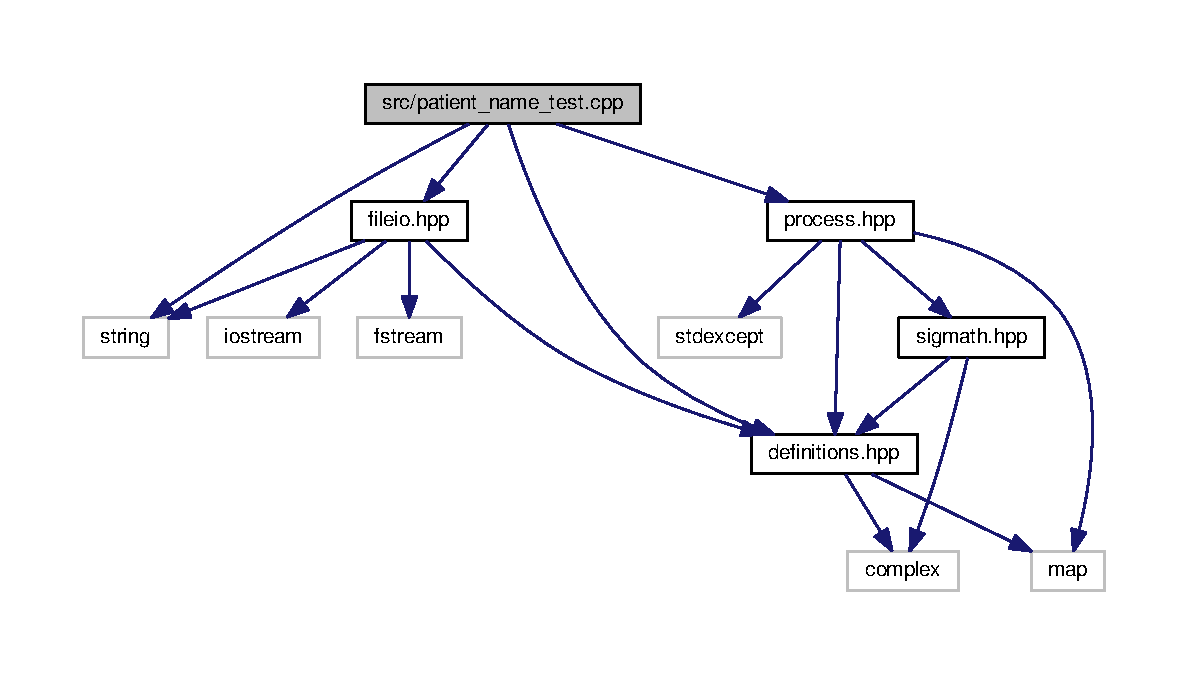
\includegraphics[width=350pt]{patient__name__test_8cpp__incl}
\end{center}
\end{figure}
\subsection*{Functions}
\begin{DoxyCompactItemize}
\item 
int \hyperlink{patient__name__test_8cpp_a3c04138a5bfe5d72780bb7e82a18e627}{main} (int argc, char $\ast$$\ast$argv)
\end{DoxyCompactItemize}


\subsection{Function Documentation}
\hypertarget{patient__name__test_8cpp_a3c04138a5bfe5d72780bb7e82a18e627}{\index{patient\+\_\+name\+\_\+test.\+cpp@{patient\+\_\+name\+\_\+test.\+cpp}!main@{main}}
\index{main@{main}!patient\+\_\+name\+\_\+test.\+cpp@{patient\+\_\+name\+\_\+test.\+cpp}}
\subsubsection[{main}]{\setlength{\rightskip}{0pt plus 5cm}int main (
\begin{DoxyParamCaption}
\item[{int}]{argc, }
\item[{char $\ast$$\ast$}]{argv}
\end{DoxyParamCaption}
)}}\label{patient__name__test_8cpp_a3c04138a5bfe5d72780bb7e82a18e627}


Definition at line \hyperlink{patient__name__test_8cpp_source_l00020}{20} of file \hyperlink{patient__name__test_8cpp_source}{patient\+\_\+name\+\_\+test.\+cpp}.



Here is the call graph for this function\+:
\nopagebreak
\begin{figure}[H]
\begin{center}
\leavevmode
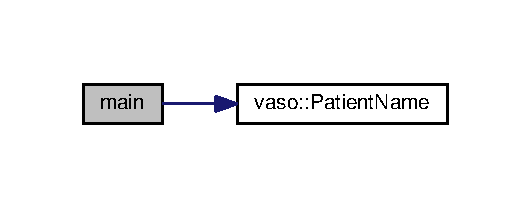
\includegraphics[width=255pt]{patient__name__test_8cpp_a3c04138a5bfe5d72780bb7e82a18e627_cgraph}
\end{center}
\end{figure}



\hypertarget{patient__name__test_8cpp_source}{\section{patient\+\_\+name\+\_\+test.\+cpp}
\label{patient__name__test_8cpp_source}\index{src/patient\+\_\+name\+\_\+test.\+cpp@{src/patient\+\_\+name\+\_\+test.\+cpp}}
}

\begin{DoxyCode}
00001 
00007 \textcolor{preprocessor}{#include <string>}
00008 
00009 \textcolor{preprocessor}{#include "\hyperlink{fileio_8hpp}{fileio.hpp}"}
00010 
00011 \textcolor{keyword}{using namespace }\hyperlink{namespacestd}{std};
00012 \textcolor{keyword}{using namespace }\hyperlink{namespaceavda}{avda};
00013 
\hypertarget{patient__name__test_8cpp_source_l00017}{}\hyperlink{patient__name__test_8cpp_a3c04138a5bfe5d72780bb7e82a18e627}{00017} \textcolor{keywordtype}{int} \hyperlink{patient__name__test_8cpp_a3c04138a5bfe5d72780bb7e82a18e627}{main}(\textcolor{keywordtype}{int} argc, \textcolor{keywordtype}{char}** argv) \{
00018     \textcolor{keywordtype}{string} filename = \hyperlink{namespaceavda_ae20728e7e8ae50bf2f74849e538841ea}{PatientName}();
00019     cout << filename;
00020 \}
\end{DoxyCode}

\hypertarget{process_8hpp}{\section{src/process.hpp File Reference}
\label{process_8hpp}\index{src/process.\+hpp@{src/process.\+hpp}}
}
{\ttfamily \#include $<$map$>$}\\*
{\ttfamily \#include $<$stdexcept$>$}\\*
{\ttfamily \#include \char`\"{}definitions.\+hpp\char`\"{}}\\*
{\ttfamily \#include \char`\"{}sigmath.\+hpp\char`\"{}}\\*
Include dependency graph for process.\+hpp\+:
\nopagebreak
\begin{figure}[H]
\begin{center}
\leavevmode
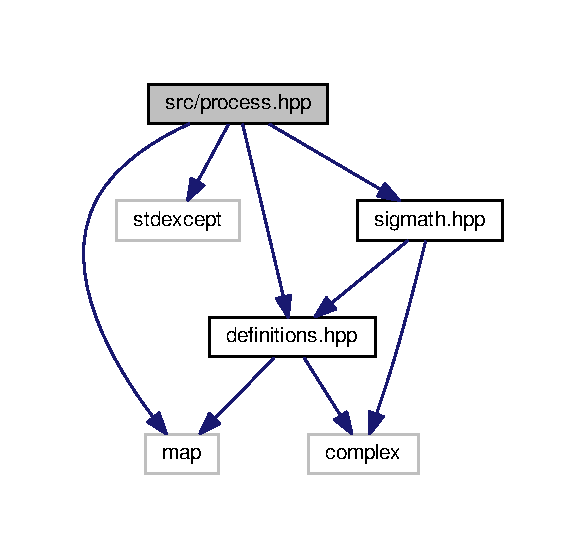
\includegraphics[width=281pt]{process_8hpp__incl}
\end{center}
\end{figure}
This graph shows which files directly or indirectly include this file\+:
\nopagebreak
\begin{figure}[H]
\begin{center}
\leavevmode
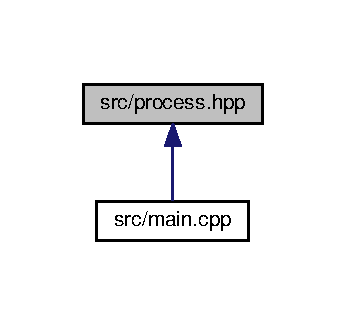
\includegraphics[width=350pt]{process_8hpp__dep__incl}
\end{center}
\end{figure}
\subsection*{Namespaces}
\begin{DoxyCompactItemize}
\item 
 \hyperlink{namespacevaso}{vaso}
\begin{DoxyCompactList}\small\item\em contains function()s related to the program's threaded processing of audio data \end{DoxyCompactList}\end{DoxyCompactItemize}
\subsection*{Functions}
\begin{DoxyCompactItemize}
\item 
std\+::map$<$ Side, \hyperlink{structDataParams}{Data\+Params} $>$ \hyperlink{namespacevaso_a0a7aa548b31b50c92be5b08bcb1df9a0}{vaso\+::\+Process} (\hyperlink{definitions_8hpp_aacdc525d6f7bddb3ae95d5c311bd06a1}{float32} $\ast$$\ast$data)
\item 
\hyperlink{structDataParams}{Data\+Params} \hyperlink{namespacevaso_a8136a2891983f7a41768330e018e3232}{vaso\+::process} (\hyperlink{definitions_8hpp_aacdc525d6f7bddb3ae95d5c311bd06a1}{float32} $\ast$data, \hyperlink{definitions_8hpp_a1134b580f8da4de94ca6b1de4d37975e}{uint32} size, \hyperlink{definitions_8hpp_aacdc525d6f7bddb3ae95d5c311bd06a1}{float32} sampling\+Rate)
\end{DoxyCompactItemize}

\hypertarget{process_8hpp_source}{\section{process.\+hpp}
\label{process_8hpp_source}\index{src/process.\+hpp@{src/process.\+hpp}}
}

\begin{DoxyCode}
00001 
00008 \textcolor{preprocessor}{#ifndef process\_H}
00009 \textcolor{preprocessor}{#define process\_H}
00010 
00011 \textcolor{preprocessor}{#include <map>}
00012 \textcolor{preprocessor}{#include <stdexcept>}
00013 
00014 \textcolor{preprocessor}{#include "\hyperlink{definitions_8hpp}{definitions.hpp}"}
00015 \textcolor{preprocessor}{#include "\hyperlink{sigmath_8hpp}{sigmath.hpp}"}
00016 
00017 \textcolor{keyword}{namespace }\hyperlink{namespaceavda}{avda} \{    
\hypertarget{process_8hpp_source_l00048}{}\hyperlink{namespaceavda_a5196cce27286d08ca144a460caee7839}{00048}     \hyperlink{structDataParams}{DataParams} \hyperlink{namespaceavda_a5196cce27286d08ca144a460caee7839}{process}(\hyperlink{definitions_8hpp_aacdc525d6f7bddb3ae95d5c311bd06a1}{float32}* data, \hyperlink{definitions_8hpp_a1134b580f8da4de94ca6b1de4d37975e}{uint32} size, 
      \hyperlink{definitions_8hpp_aacdc525d6f7bddb3ae95d5c311bd06a1}{float32} samplingRate) \{
00049         \textcolor{keywordflow}{if}((size & (size - 1) != 0) || size < 2) \{
00050             \textcolor{keywordflow}{throw} std::invalid\_argument(
00051                     \textcolor{stringliteral}{"The number of samples is not a power of two!"});
00052         \}
00053 
00054         \textcolor{comment}{// declare function-scoped variables}
00055         \hyperlink{definitions_8hpp_a1134b580f8da4de94ca6b1de4d37975e}{uint32} freqSize = size / 2;
00056         \hyperlink{definitions_8hpp_a960be6b6614c08090c16574dba10a421}{cfloat32}* cdata = (\hyperlink{definitions_8hpp_a960be6b6614c08090c16574dba10a421}{cfloat32}*)std::malloc(size * \textcolor{keyword}{sizeof}(
      \hyperlink{definitions_8hpp_a960be6b6614c08090c16574dba10a421}{cfloat32}));
00057         \hyperlink{definitions_8hpp_aacdc525d6f7bddb3ae95d5c311bd06a1}{float32}* fdata = (\hyperlink{definitions_8hpp_aacdc525d6f7bddb3ae95d5c311bd06a1}{float32}*)std::malloc(freqSize * \textcolor{keyword}{sizeof}(
      \hyperlink{definitions_8hpp_aacdc525d6f7bddb3ae95d5c311bd06a1}{float32}));
00058         \hyperlink{definitions_8hpp_aacdc525d6f7bddb3ae95d5c311bd06a1}{float32}* origdata = (\hyperlink{definitions_8hpp_aacdc525d6f7bddb3ae95d5c311bd06a1}{float32}*)std::malloc(freqSize * \textcolor{keyword}{sizeof}(
      \hyperlink{definitions_8hpp_aacdc525d6f7bddb3ae95d5c311bd06a1}{float32}));
00059 
00060         \textcolor{comment}{// convert data to complex numbers for fft()}
00061         \textcolor{keywordflow}{for}(\hyperlink{definitions_8hpp_a1134b580f8da4de94ca6b1de4d37975e}{uint32} i = 0; i < size; i++) \{
00062             cdata[i] = data[i];
00063         \}
00064     
00065         \textcolor{comment}{// find frequency spectrum in relative decibels}
00066         \hyperlink{namespaceavda_a33a1102422421212ac6b9387c896e864}{fft}(cdata, size);
00067         \hyperlink{namespaceavda_a213bd6384fc9a330e4db2cecdbcd73ee}{mag}(cdata, fdata, freqSize);
00068         \hyperlink{structMaximum}{Maximum} maximum = \hyperlink{namespaceavda_aa82021c3ee552773c060b1a39caf8aaa}{max}(fdata, freqSize);
00069 
00070         \textcolor{keywordflow}{for}(\hyperlink{definitions_8hpp_a1134b580f8da4de94ca6b1de4d37975e}{uint32} i = 0; i < freqSize; i++) \{
00071             fdata[i] /= maximum.\hyperlink{structMaximum_aa7e84cbf37b694670142670014366969}{value};
00072         \}
00073 
00074         \hyperlink{namespaceavda_a9c0b7f832eace3cbc9c5dddea2ecc9d5}{decibels}(fdata, freqSize);
00075 
00076         \textcolor{keywordflow}{for}(\hyperlink{definitions_8hpp_a1134b580f8da4de94ca6b1de4d37975e}{uint32} i = 0; i < freqSize; i++) \{
00077             origdata[i] = fdata[i];
00078         \}
00079 
00080         \textcolor{comment}{/*}
00081 \textcolor{comment}{         * Run spectrum values through moving-average filter to smooth the}
00082 \textcolor{comment}{         * curve and make it easier to determine the derivative.}
00083 \textcolor{comment}{         */}
00084         \hyperlink{namespaceavda_a22583ba7f11b69c955b13155bf9a739d}{smooth}(fdata, freqSize, 20);
00085 
00086         \textcolor{comment}{/*}
00087 \textcolor{comment}{         * Find the derivative of the smoothed spectrum. Bote that both this}
00088 \textcolor{comment}{         * filter and the previous are necessary to the algorithm.}
00089 \textcolor{comment}{         */}
00090         \hyperlink{namespaceavda_a3e9b92cfa9d76c4c363e8ed8a4c1a2ce}{diff}(fdata, freqSize);
00091         \hyperlink{namespaceavda_a22583ba7f11b69c955b13155bf9a739d}{smooth}(fdata, freqSize, 100);
00092         \hyperlink{namespaceavda_aa771d0ed99fc4954c643ea71e91905bf}{absolute}(fdata, freqSize);
00093 
00094         \textcolor{comment}{// find the parameters of this specific recording}
00095         \hyperlink{definitions_8hpp_a05f6b0ae8f6a6e135b0e290c25fe0e4e}{uint16} offset = 1000;
00096         \hyperlink{namespaceavda_aa771d0ed99fc4954c643ea71e91905bf}{absolute}(&fdata[offset], freqSize - offset);
00097         maximum = \hyperlink{namespaceavda_aa82021c3ee552773c060b1a39caf8aaa}{max}(&fdata[offset], freqSize - offset);
00098         \hyperlink{definitions_8hpp_a1134b580f8da4de94ca6b1de4d37975e}{uint32} index = maximum.\hyperlink{structMaximum_a2e6aef03795cd285fe542d0861c6e3b5}{index} + offset;
00099         
00100         \hyperlink{structDataParams}{DataParams} params;
00101         params.\hyperlink{structDataParams_a12566e017407647bc8287d62554ad3fb}{freq} = index * (float)\hyperlink{definitions_8hpp_a8ace559345ecba7978591ac2ef22aea4}{SAMPLE\_FREQ} / freqSize / 2;
00102         params.\hyperlink{structDataParams_a4efd1d2231c6fa7c878c9d5e1650738f}{noise} = \hyperlink{namespaceavda_a2a830f24a59aa2538ea82f6e000cce61}{average}(&origdata[index + offset],
00103                 freqSize - offset - index);
00104 
00105         free(cdata);
00106         free(fdata);
00107 
00108         \textcolor{keywordflow}{return} params;
00109     \}
00110 \}
00111 
00112 \textcolor{preprocessor}{#endif}
\end{DoxyCode}

\hypertarget{process__test_8cpp}{\section{src/process\+\_\+test.cpp File Reference}
\label{process__test_8cpp}\index{src/process\+\_\+test.\+cpp@{src/process\+\_\+test.\+cpp}}
}
{\ttfamily \#include $<$cstdio$>$}\\*
{\ttfamily \#include $<$cstdlib$>$}\\*
{\ttfamily \#include $<$fcntl.\+h$>$}\\*
{\ttfamily \#include $<$iostream$>$}\\*
{\ttfamily \#include $<$string$>$}\\*
{\ttfamily \#include $<$unistd.\+h$>$}\\*
{\ttfamily \#include \char`\"{}definitions.\+hpp\char`\"{}}\\*
{\ttfamily \#include \char`\"{}process.\+hpp\char`\"{}}\\*
Include dependency graph for process\+\_\+test.\+cpp\+:
\nopagebreak
\begin{figure}[H]
\begin{center}
\leavevmode
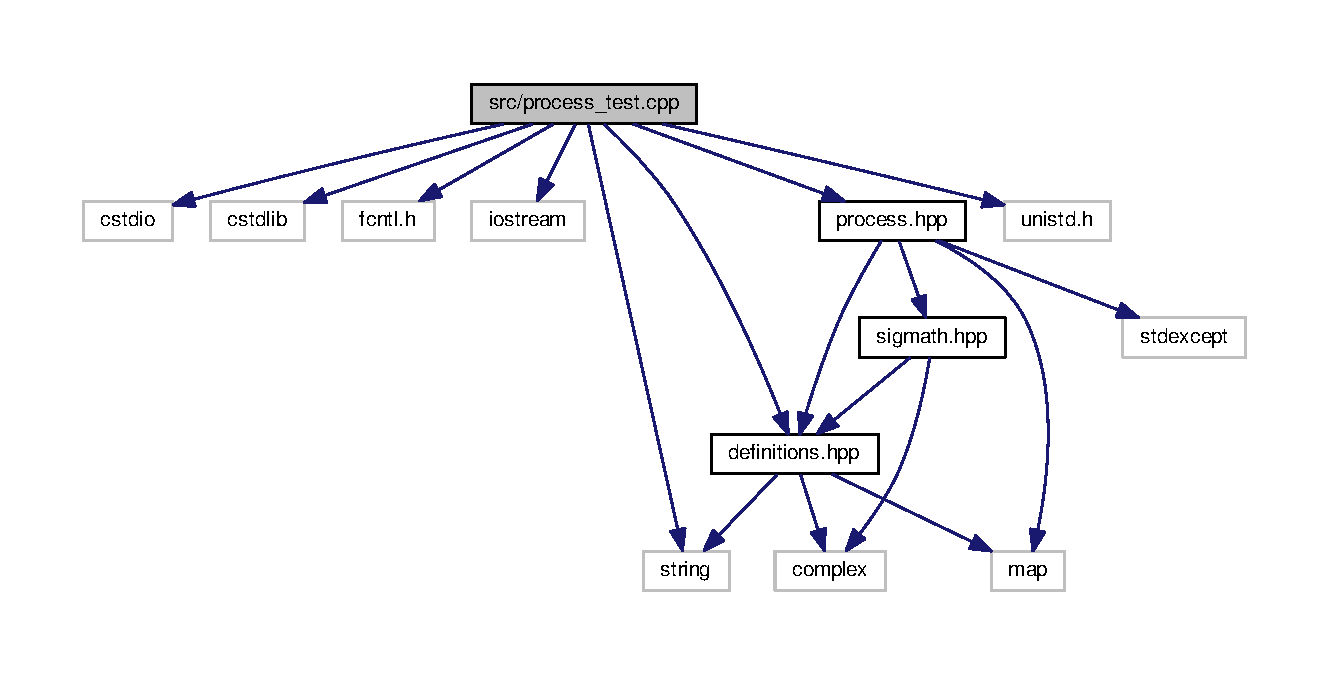
\includegraphics[width=350pt]{process__test_8cpp__incl}
\end{center}
\end{figure}
\subsection*{Macros}
\begin{DoxyCompactItemize}
\item 
\#define \hyperlink{process__test_8cpp_a698c124f1c293f98840449d6c5b9d984}{C\+O\+U\+N\+T}~131072
\end{DoxyCompactItemize}
\subsection*{Functions}
\begin{DoxyCompactItemize}
\item 
int \hyperlink{process__test_8cpp_a3c04138a5bfe5d72780bb7e82a18e627}{main} (int argc, char $\ast$$\ast$argv)
\end{DoxyCompactItemize}


\subsection{Detailed Description}
\begin{DoxyAuthor}{Author}
Samuel Andrew Wisner, \href{mailto:awisner94@gmail.com}{\tt awisner94@gmail.\+com} 

Nicholas K. Nolan 
\end{DoxyAuthor}


Definition in file \hyperlink{process__test_8cpp_source}{process\+\_\+test.\+cpp}.



\subsection{Macro Definition Documentation}
\hypertarget{process__test_8cpp_a698c124f1c293f98840449d6c5b9d984}{\index{process\+\_\+test.\+cpp@{process\+\_\+test.\+cpp}!C\+O\+U\+N\+T@{C\+O\+U\+N\+T}}
\index{C\+O\+U\+N\+T@{C\+O\+U\+N\+T}!process\+\_\+test.\+cpp@{process\+\_\+test.\+cpp}}
\subsubsection[{C\+O\+U\+N\+T}]{\setlength{\rightskip}{0pt plus 5cm}\#define C\+O\+U\+N\+T~131072}}\label{process__test_8cpp_a698c124f1c293f98840449d6c5b9d984}


Definition at line \hyperlink{process__test_8cpp_source_l00018}{18} of file \hyperlink{process__test_8cpp_source}{process\+\_\+test.\+cpp}.



\subsection{Function Documentation}
\hypertarget{process__test_8cpp_a3c04138a5bfe5d72780bb7e82a18e627}{\index{process\+\_\+test.\+cpp@{process\+\_\+test.\+cpp}!main@{main}}
\index{main@{main}!process\+\_\+test.\+cpp@{process\+\_\+test.\+cpp}}
\subsubsection[{main}]{\setlength{\rightskip}{0pt plus 5cm}int main (
\begin{DoxyParamCaption}
\item[{int}]{argc, }
\item[{char $\ast$$\ast$}]{argv}
\end{DoxyParamCaption}
)}}\label{process__test_8cpp_a3c04138a5bfe5d72780bb7e82a18e627}


Definition at line \hyperlink{process__test_8cpp_source_l00026}{26} of file \hyperlink{process__test_8cpp_source}{process\+\_\+test.\+cpp}.



Here is the call graph for this function\+:
\nopagebreak
\begin{figure}[H]
\begin{center}
\leavevmode
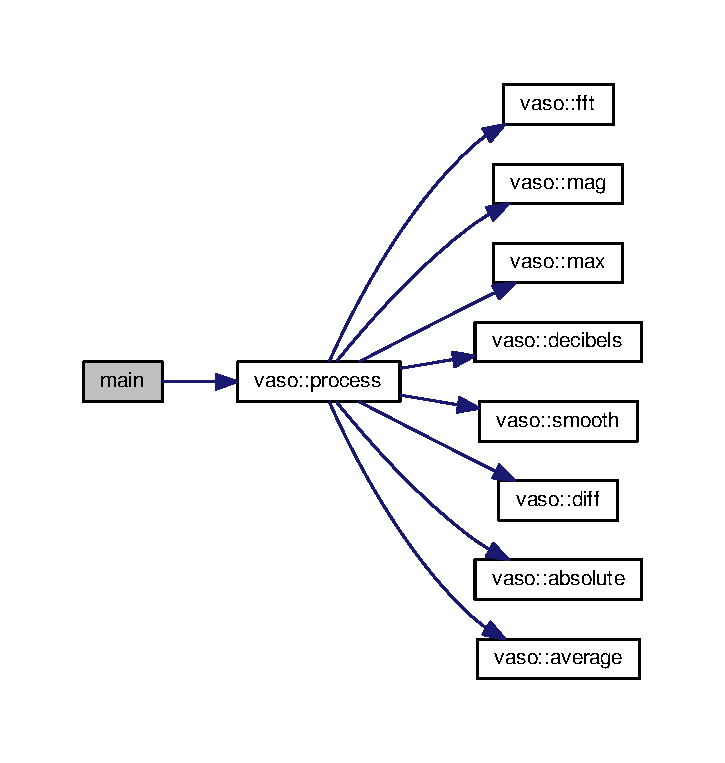
\includegraphics[width=348pt]{process__test_8cpp_a3c04138a5bfe5d72780bb7e82a18e627_cgraph}
\end{center}
\end{figure}



\hypertarget{process__test_8cpp_source}{\section{process\+\_\+test.\+cpp}
\label{process__test_8cpp_source}\index{src/process\+\_\+test.\+cpp@{src/process\+\_\+test.\+cpp}}
}

\begin{DoxyCode}
00001 
00008 \textcolor{preprocessor}{#include <cstdio>}
00009 \textcolor{preprocessor}{#include <cstdlib>}
00010 \textcolor{preprocessor}{#include <fcntl.h>}
00011 \textcolor{preprocessor}{#include <iostream>}
00012 \textcolor{preprocessor}{#include <string>}
00013 \textcolor{preprocessor}{#include <unistd.h>}
00014 
00015 \textcolor{preprocessor}{#include "\hyperlink{definitions_8hpp}{definitions.hpp}"}
00016 \textcolor{preprocessor}{#include "\hyperlink{process_8hpp}{process.hpp}"}
00017 
\hypertarget{process__test_8cpp_source_l00018}{}\hyperlink{process__test_8cpp_a698c124f1c293f98840449d6c5b9d984}{00018} \textcolor{preprocessor}{#define COUNT 131072}
00019 
00020 \textcolor{keyword}{using namespace }\hyperlink{namespacestd}{std};
00021 \textcolor{keyword}{using namespace }\hyperlink{namespacevaso}{vaso};
00022 
\hypertarget{process__test_8cpp_source_l00026}{}\hyperlink{process__test_8cpp_a3c04138a5bfe5d72780bb7e82a18e627}{00026} \textcolor{keywordtype}{int} \hyperlink{process__test_8cpp_a3c04138a5bfe5d72780bb7e82a18e627}{main}(\textcolor{keywordtype}{int} argc, \textcolor{keywordtype}{char}** argv) \{
00027     \textcolor{keywordtype}{int} file = open(\textcolor{stringliteral}{"/home/pi/vaso/etc/audio/test.raw"}, O\_RDONLY);
00028 
00029     \textcolor{keywordflow}{if}(file < 0) \{
00030         cerr << \textcolor{stringliteral}{"File unreadable!"} << endl;
00031         \textcolor{keywordflow}{return} -1;
00032     \}
00033 
00034     \hyperlink{definitions_8hpp_aacdc525d6f7bddb3ae95d5c311bd06a1}{float32}* buffer = (\hyperlink{definitions_8hpp_aacdc525d6f7bddb3ae95d5c311bd06a1}{float32}*)malloc(\hyperlink{process__test_8cpp_a698c124f1c293f98840449d6c5b9d984}{COUNT} * \textcolor{keyword}{sizeof}(\hyperlink{definitions_8hpp_aacdc525d6f7bddb3ae95d5c311bd06a1}{float32}));
00035     \textcolor{keywordtype}{int} charRead = read(file, buffer, \hyperlink{process__test_8cpp_a698c124f1c293f98840449d6c5b9d984}{COUNT} * \textcolor{keyword}{sizeof}(\hyperlink{definitions_8hpp_aacdc525d6f7bddb3ae95d5c311bd06a1}{float32}));
00036 
00037     \textcolor{keywordflow}{if}(charRead < \hyperlink{process__test_8cpp_a698c124f1c293f98840449d6c5b9d984}{COUNT}) \{
00038         cerr << \textcolor{stringliteral}{"Too few bytes read!"} << endl;
00039         \textcolor{keywordflow}{return} -1;
00040     \}
00041 
00042     close(file);
00043 
00044     \hyperlink{structDataParams}{DataParams} params = \hyperlink{namespacevaso_a8136a2891983f7a41768330e018e3232}{process}(buffer, \hyperlink{process__test_8cpp_a698c124f1c293f98840449d6c5b9d984}{COUNT}, \hyperlink{definitions_8hpp_a8ace559345ecba7978591ac2ef22aea4}{SAMPLE\_FREQ});
00045     free(buffer);
00046     cout << \textcolor{stringliteral}{"Cutoff: "} << params.\hyperlink{structDataParams_a12566e017407647bc8287d62554ad3fb}{freq} << endl;
00047     cout << \textcolor{stringliteral}{"Noise: "} << params.\hyperlink{structDataParams_a4efd1d2231c6fa7c878c9d5e1650738f}{noise} << endl;
00048 \}
\end{DoxyCode}

\hypertarget{sigmath_8hpp}{\section{src/sigmath.hpp File Reference}
\label{sigmath_8hpp}\index{src/sigmath.\+hpp@{src/sigmath.\+hpp}}
}
{\ttfamily \#include $<$complex$>$}\\*
{\ttfamily \#include \char`\"{}definitions.\+hpp\char`\"{}}\\*
Include dependency graph for sigmath.\+hpp\+:
\nopagebreak
\begin{figure}[H]
\begin{center}
\leavevmode
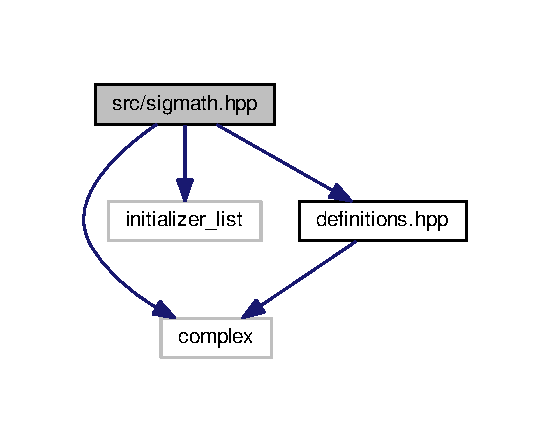
\includegraphics[width=197pt]{sigmath_8hpp__incl}
\end{center}
\end{figure}
This graph shows which files directly or indirectly include this file\+:
\nopagebreak
\begin{figure}[H]
\begin{center}
\leavevmode
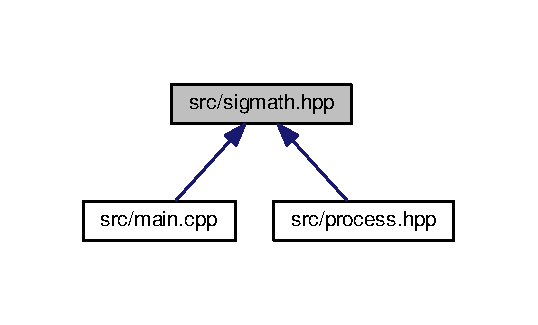
\includegraphics[width=258pt]{sigmath_8hpp__dep__incl}
\end{center}
\end{figure}
\subsection*{Namespaces}
\begin{DoxyCompactItemize}
\item 
 \hyperlink{namespacevaso}{vaso}
\begin{DoxyCompactList}\small\item\em contains functions related to the file I/\+O use in this program \end{DoxyCompactList}\end{DoxyCompactItemize}
\subsection*{Functions}
\begin{DoxyCompactItemize}
\item 
void \hyperlink{namespacevaso_a6ca90add966ce1773fc59a6883e6cd0c}{vaso\+::absolute} (\hyperlink{definitions_8hpp_aacdc525d6f7bddb3ae95d5c311bd06a1}{float32} $\ast$data, \hyperlink{definitions_8hpp_a1134b580f8da4de94ca6b1de4d37975e}{uint32} size)
\item 
\hyperlink{definitions_8hpp_aacdc525d6f7bddb3ae95d5c311bd06a1}{float32} \hyperlink{namespacevaso_ad3205136b1cd04b4c6b9d7be73661796}{vaso\+::average} (\hyperlink{definitions_8hpp_aacdc525d6f7bddb3ae95d5c311bd06a1}{float32} $\ast$data, \hyperlink{definitions_8hpp_a1134b580f8da4de94ca6b1de4d37975e}{uint32} size)
\item 
\hyperlink{structDataParams}{Data\+Params} \hyperlink{namespacevaso_a376413e791defec04a0faf329be1cbf4}{vaso\+::average} (\hyperlink{structDataParams}{Data\+Params} $\ast$params, \hyperlink{definitions_8hpp_adde6aaee8457bee49c2a92621fe22b79}{uint8} size)
\item 
void \hyperlink{namespacevaso_a9d0e5d69685ee494d286db6ece005156}{vaso\+::average} (\hyperlink{definitions_8hpp_aacdc525d6f7bddb3ae95d5c311bd06a1}{float32} $\ast$data, \hyperlink{definitions_8hpp_aacdc525d6f7bddb3ae95d5c311bd06a1}{float32} $\ast$avg, \hyperlink{definitions_8hpp_adde6aaee8457bee49c2a92621fe22b79}{uint8} count, \hyperlink{definitions_8hpp_a1134b580f8da4de94ca6b1de4d37975e}{uint32} size)
\item 
void \hyperlink{namespacevaso_af9bb2211cf3478333dfc1873bf316263}{vaso\+::decibels} (\hyperlink{definitions_8hpp_aacdc525d6f7bddb3ae95d5c311bd06a1}{float32} $\ast$data, \hyperlink{definitions_8hpp_a1134b580f8da4de94ca6b1de4d37975e}{uint32} size)
\item 
void \hyperlink{namespacevaso_a7d108bce812e906d8b1810815774c7ea}{vaso\+::diff} (\hyperlink{definitions_8hpp_aacdc525d6f7bddb3ae95d5c311bd06a1}{float32} $\ast$data, \hyperlink{definitions_8hpp_a1134b580f8da4de94ca6b1de4d37975e}{uint32} size)
\item 
void \hyperlink{namespacevaso_af74f08a8afd7967b6c2b3c2b0e5fb1e9}{vaso\+::fft} (\hyperlink{definitions_8hpp_a960be6b6614c08090c16574dba10a421}{cfloat32} $\ast$data, \hyperlink{definitions_8hpp_a1134b580f8da4de94ca6b1de4d37975e}{uint32} size)
\item 
void \hyperlink{namespacevaso_a5d355b5c326a852e2ce95c258450898c}{vaso\+::mag} (\hyperlink{definitions_8hpp_a960be6b6614c08090c16574dba10a421}{cfloat32} $\ast$orig, \hyperlink{definitions_8hpp_aacdc525d6f7bddb3ae95d5c311bd06a1}{float32} $\ast$newmags, \hyperlink{definitions_8hpp_a1134b580f8da4de94ca6b1de4d37975e}{uint32} size)
\item 
\hyperlink{structMaximum}{Maximum} \hyperlink{namespacevaso_a122846d728be312454a452d379915e10}{vaso\+::max} (\hyperlink{definitions_8hpp_aacdc525d6f7bddb3ae95d5c311bd06a1}{float32} $\ast$data, \hyperlink{definitions_8hpp_a1134b580f8da4de94ca6b1de4d37975e}{uint32} size)
\item 
void \hyperlink{namespacevaso_a5b7fc1a58199e2cac989f417a9faa1ce}{vaso\+::smooth} (\hyperlink{definitions_8hpp_aacdc525d6f7bddb3ae95d5c311bd06a1}{float32} $\ast$data, \hyperlink{definitions_8hpp_a1134b580f8da4de94ca6b1de4d37975e}{uint32} size, \hyperlink{definitions_8hpp_a05f6b0ae8f6a6e135b0e290c25fe0e4e}{uint16} order)
\end{DoxyCompactItemize}

\hypertarget{sigmath_8hpp_source}{\section{sigmath.\+hpp}
\label{sigmath_8hpp_source}\index{src/sigmath.\+hpp@{src/sigmath.\+hpp}}
}

\begin{DoxyCode}
00001 
00008 \textcolor{preprocessor}{#ifndef sigmath\_H}
00009 \textcolor{preprocessor}{#define sigmath\_H}
00010 
00011 \textcolor{preprocessor}{#include <complex>}
00012 
00013 \textcolor{preprocessor}{#include "\hyperlink{definitions_8hpp}{definitions.hpp}"}
00014 
00015 \textcolor{keyword}{namespace }\hyperlink{namespacevaso}{vaso} \{
00016     \textcolor{comment}{// PROTOTYPES}
00017 
00026     \textcolor{keywordtype}{void} \hyperlink{namespacevaso_a6ca90add966ce1773fc59a6883e6cd0c}{absolute}(\hyperlink{definitions_8hpp_aacdc525d6f7bddb3ae95d5c311bd06a1}{float32}* data, \hyperlink{definitions_8hpp_a1134b580f8da4de94ca6b1de4d37975e}{uint32} size);
00027 
00037     \hyperlink{definitions_8hpp_aacdc525d6f7bddb3ae95d5c311bd06a1}{float32} \hyperlink{namespacevaso_ad3205136b1cd04b4c6b9d7be73661796}{average}(\hyperlink{definitions_8hpp_aacdc525d6f7bddb3ae95d5c311bd06a1}{float32}* data, \hyperlink{definitions_8hpp_a1134b580f8da4de94ca6b1de4d37975e}{uint32} size);
00038 
00049     \hyperlink{structDataParams}{DataParams} \hyperlink{namespacevaso_ad3205136b1cd04b4c6b9d7be73661796}{average}(\hyperlink{structDataParams}{DataParams}* params, \hyperlink{definitions_8hpp_adde6aaee8457bee49c2a92621fe22b79}{uint8} size);
00050 
00067     \textcolor{keywordtype}{void} \hyperlink{namespacevaso_ad3205136b1cd04b4c6b9d7be73661796}{average}(\hyperlink{definitions_8hpp_aacdc525d6f7bddb3ae95d5c311bd06a1}{float32}* data, \hyperlink{definitions_8hpp_aacdc525d6f7bddb3ae95d5c311bd06a1}{float32}* avg, \hyperlink{definitions_8hpp_adde6aaee8457bee49c2a92621fe22b79}{uint8} count, 
      \hyperlink{definitions_8hpp_a1134b580f8da4de94ca6b1de4d37975e}{uint32} size);
00068 
00080     \textcolor{keywordtype}{void} \hyperlink{namespacevaso_af9bb2211cf3478333dfc1873bf316263}{decibels}(\hyperlink{definitions_8hpp_aacdc525d6f7bddb3ae95d5c311bd06a1}{float32}* data, \hyperlink{definitions_8hpp_a1134b580f8da4de94ca6b1de4d37975e}{uint32} size);
00081 
00090     \textcolor{keywordtype}{void} \hyperlink{namespacevaso_a7d108bce812e906d8b1810815774c7ea}{diff}(\hyperlink{definitions_8hpp_aacdc525d6f7bddb3ae95d5c311bd06a1}{float32}* data, \hyperlink{definitions_8hpp_a1134b580f8da4de94ca6b1de4d37975e}{uint32} size);
00091 
00103     \textcolor{keywordtype}{void} \hyperlink{namespacevaso_af74f08a8afd7967b6c2b3c2b0e5fb1e9}{fft}(\hyperlink{definitions_8hpp_a960be6b6614c08090c16574dba10a421}{cfloat32}* data, \hyperlink{definitions_8hpp_a1134b580f8da4de94ca6b1de4d37975e}{uint32} size);
00104 
00114     \textcolor{keywordtype}{void} \hyperlink{namespacevaso_a5d355b5c326a852e2ce95c258450898c}{mag}(\hyperlink{definitions_8hpp_a960be6b6614c08090c16574dba10a421}{cfloat32}* orig, \hyperlink{definitions_8hpp_aacdc525d6f7bddb3ae95d5c311bd06a1}{float32}* newmags, \hyperlink{definitions_8hpp_a1134b580f8da4de94ca6b1de4d37975e}{uint32} size);
00115 
00125     \hyperlink{structMaximum}{Maximum} \hyperlink{namespacevaso_a122846d728be312454a452d379915e10}{max}(\hyperlink{definitions_8hpp_aacdc525d6f7bddb3ae95d5c311bd06a1}{float32}* data, \hyperlink{definitions_8hpp_a1134b580f8da4de94ca6b1de4d37975e}{uint32} size);
00126 
00137     \textcolor{keywordtype}{void} \hyperlink{namespacevaso_a5b7fc1a58199e2cac989f417a9faa1ce}{smooth}(\hyperlink{definitions_8hpp_aacdc525d6f7bddb3ae95d5c311bd06a1}{float32}* data, \hyperlink{definitions_8hpp_a1134b580f8da4de94ca6b1de4d37975e}{uint32} size, \hyperlink{definitions_8hpp_a05f6b0ae8f6a6e135b0e290c25fe0e4e}{uint16} order);
00138 
00139     \textcolor{comment}{// DEFINITIONS}
00140 
\hypertarget{sigmath_8hpp_source_l00141}{}\hyperlink{namespacevaso_a6ca90add966ce1773fc59a6883e6cd0c}{00141}     \textcolor{keywordtype}{void} \hyperlink{namespacevaso_a6ca90add966ce1773fc59a6883e6cd0c}{absolute}(\hyperlink{definitions_8hpp_aacdc525d6f7bddb3ae95d5c311bd06a1}{float32}* data, \hyperlink{definitions_8hpp_a1134b580f8da4de94ca6b1de4d37975e}{uint32} size) \{
00142 
00143     \}
00144 
\hypertarget{sigmath_8hpp_source_l00145}{}\hyperlink{namespacevaso_ad3205136b1cd04b4c6b9d7be73661796}{00145}     \hyperlink{definitions_8hpp_aacdc525d6f7bddb3ae95d5c311bd06a1}{float32} \hyperlink{namespacevaso_ad3205136b1cd04b4c6b9d7be73661796}{average}(\hyperlink{definitions_8hpp_aacdc525d6f7bddb3ae95d5c311bd06a1}{float32}* data, \hyperlink{definitions_8hpp_a1134b580f8da4de94ca6b1de4d37975e}{uint32} size) \{
00146 
00147     \}
00148 
\hypertarget{sigmath_8hpp_source_l00149}{}\hyperlink{namespacevaso_a376413e791defec04a0faf329be1cbf4}{00149}     \hyperlink{structDataParams}{DataParams} \hyperlink{namespacevaso_ad3205136b1cd04b4c6b9d7be73661796}{average}(\hyperlink{structDataParams}{DataParams}* params, \hyperlink{definitions_8hpp_adde6aaee8457bee49c2a92621fe22b79}{uint8} size) \{
00150 
00151     \}
00152 
\hypertarget{sigmath_8hpp_source_l00153}{}\hyperlink{namespacevaso_a9d0e5d69685ee494d286db6ece005156}{00153}     \textcolor{keywordtype}{void} \hyperlink{namespacevaso_ad3205136b1cd04b4c6b9d7be73661796}{average}(\hyperlink{definitions_8hpp_aacdc525d6f7bddb3ae95d5c311bd06a1}{float32}* data, \hyperlink{definitions_8hpp_aacdc525d6f7bddb3ae95d5c311bd06a1}{float32}* avg, \hyperlink{definitions_8hpp_adde6aaee8457bee49c2a92621fe22b79}{uint8} count, 
      \hyperlink{definitions_8hpp_a1134b580f8da4de94ca6b1de4d37975e}{uint32} size) \{
00154         \textcolor{comment}{// data is an array. Access like so: data[index]}
00155     \}
00156 
\hypertarget{sigmath_8hpp_source_l00157}{}\hyperlink{namespacevaso_af9bb2211cf3478333dfc1873bf316263}{00157}     \textcolor{keywordtype}{void} \hyperlink{namespacevaso_af9bb2211cf3478333dfc1873bf316263}{decibels}(\hyperlink{definitions_8hpp_aacdc525d6f7bddb3ae95d5c311bd06a1}{float32}* data, \hyperlink{definitions_8hpp_a1134b580f8da4de94ca6b1de4d37975e}{uint32} size) \{
00158         \textcolor{keywordflow}{for}(\hyperlink{definitions_8hpp_a1134b580f8da4de94ca6b1de4d37975e}{uint32} i = 0; i < size; i++) \{
00159             data[i] = 20 * log10(data[i]);
00160         \}
00161     \}
00162 
\hypertarget{sigmath_8hpp_source_l00163}{}\hyperlink{namespacevaso_a7d108bce812e906d8b1810815774c7ea}{00163}     \textcolor{keywordtype}{void} \hyperlink{namespacevaso_a7d108bce812e906d8b1810815774c7ea}{diff}(\hyperlink{definitions_8hpp_aacdc525d6f7bddb3ae95d5c311bd06a1}{float32}* data, \hyperlink{definitions_8hpp_a1134b580f8da4de94ca6b1de4d37975e}{uint32} size) \{
00164 
00165     \}
00166 
\hypertarget{sigmath_8hpp_source_l00167}{}\hyperlink{namespacevaso_af74f08a8afd7967b6c2b3c2b0e5fb1e9}{00167}     \textcolor{keywordtype}{void} \hyperlink{namespacevaso_af74f08a8afd7967b6c2b3c2b0e5fb1e9}{fft}(\hyperlink{definitions_8hpp_a960be6b6614c08090c16574dba10a421}{cfloat32}* data, \hyperlink{definitions_8hpp_a1134b580f8da4de94ca6b1de4d37975e}{uint32} size) \{
00168         \textcolor{comment}{// DFT}
00169         \hyperlink{definitions_8hpp_a1134b580f8da4de94ca6b1de4d37975e}{uint32} k = size;
00170         \hyperlink{definitions_8hpp_a1134b580f8da4de94ca6b1de4d37975e}{uint32} n;
00171         \hyperlink{definitions_8hpp_aacdc525d6f7bddb3ae95d5c311bd06a1}{float32} thetaT = M\_PI / size;
00172         \hyperlink{definitions_8hpp_a960be6b6614c08090c16574dba10a421}{cfloat32} phiT(cos(thetaT), sin(thetaT));
00173         \hyperlink{definitions_8hpp_a960be6b6614c08090c16574dba10a421}{cfloat32} T;
00174 
00175         \textcolor{keywordflow}{while}(k > 1) \{
00176             n = k;
00177             k >>= 1;
00178             phiT = phiT * phiT;
00179             T = 1.0L;
00180 
00181             \textcolor{keywordflow}{for}(\hyperlink{definitions_8hpp_a1134b580f8da4de94ca6b1de4d37975e}{uint32} l = 0; l < k; l++) \{
00182                 \textcolor{keywordflow}{for}(\hyperlink{definitions_8hpp_a1134b580f8da4de94ca6b1de4d37975e}{uint32} a = l; a < size; a += n) \{
00183                     \hyperlink{definitions_8hpp_a1134b580f8da4de94ca6b1de4d37975e}{uint32} b = a + k;
00184                     \hyperlink{definitions_8hpp_a960be6b6614c08090c16574dba10a421}{cfloat32} t = data[a] -data[b];
00185                     data[a] +=data[b];
00186                     data[b] = t * T;
00187                 \}
00188 
00189                 T *= phiT;
00190             \}
00191         \}
00192 
00193         \textcolor{comment}{// Decimate}
00194         \hyperlink{definitions_8hpp_a1134b580f8da4de94ca6b1de4d37975e}{uint32} m = (\hyperlink{definitions_8hpp_a1134b580f8da4de94ca6b1de4d37975e}{uint32})log2(size);
00195 
00196         \textcolor{keywordflow}{for}(\hyperlink{definitions_8hpp_a1134b580f8da4de94ca6b1de4d37975e}{uint32} a = 0; a < size; a++) \{
00197             \hyperlink{definitions_8hpp_a1134b580f8da4de94ca6b1de4d37975e}{uint32} b = a;
00198 
00199             \textcolor{comment}{// Reverse bits}
00200             b = (((b & 0xaaaaaaaa) >> 1) | ((b & 0x55555555) << 1));
00201             b = (((b & 0xcccccccc) >> 2) | ((b & 0x33333333) << 2));
00202             b = (((b & 0xf0f0f0f0) >> 4) | ((b & 0x0f0f0f0f) << 4));
00203             b = (((b & 0xff00ff00) >> 8) | ((b & 0x00ff00ff) << 8));
00204             b = ((b >> 16) | (b << 16)) >> (32 - m);
00205 
00206             \textcolor{keywordflow}{if} (b > a)
00207             \{
00208                 \hyperlink{definitions_8hpp_a960be6b6614c08090c16574dba10a421}{cfloat32} t = data[a];
00209                 data[a] =data[b];
00210                 data[b] = t;
00211             \}
00212         \}
00213     \}
00214 
\hypertarget{sigmath_8hpp_source_l00215}{}\hyperlink{namespacevaso_a5d355b5c326a852e2ce95c258450898c}{00215}     \textcolor{keywordtype}{void} \hyperlink{namespacevaso_a5d355b5c326a852e2ce95c258450898c}{mag}(\hyperlink{definitions_8hpp_a960be6b6614c08090c16574dba10a421}{cfloat32}* orig, \hyperlink{definitions_8hpp_aacdc525d6f7bddb3ae95d5c311bd06a1}{float32}* newmags, \hyperlink{definitions_8hpp_a1134b580f8da4de94ca6b1de4d37975e}{uint32} size) \{
00216 
00217     \}
00218 
\hypertarget{sigmath_8hpp_source_l00219}{}\hyperlink{namespacevaso_a122846d728be312454a452d379915e10}{00219}     \hyperlink{structMaximum}{Maximum} \hyperlink{namespacevaso_a122846d728be312454a452d379915e10}{max}(\hyperlink{definitions_8hpp_aacdc525d6f7bddb3ae95d5c311bd06a1}{float32}* data, \hyperlink{definitions_8hpp_a1134b580f8da4de94ca6b1de4d37975e}{uint32} size) \{
00220 
00221     \}
00222 
\hypertarget{sigmath_8hpp_source_l00223}{}\hyperlink{namespacevaso_a5b7fc1a58199e2cac989f417a9faa1ce}{00223}     \textcolor{keywordtype}{void} \hyperlink{namespacevaso_a5b7fc1a58199e2cac989f417a9faa1ce}{smooth}(\hyperlink{definitions_8hpp_aacdc525d6f7bddb3ae95d5c311bd06a1}{float32}* data, \hyperlink{definitions_8hpp_a1134b580f8da4de94ca6b1de4d37975e}{uint32} size, \hyperlink{definitions_8hpp_a05f6b0ae8f6a6e135b0e290c25fe0e4e}{uint16} order) \{
00224         \hyperlink{definitions_8hpp_aacdc525d6f7bddb3ae95d5c311bd06a1}{float32} coeff = 1 / (\hyperlink{definitions_8hpp_aacdc525d6f7bddb3ae95d5c311bd06a1}{float32})order;
00225         \hyperlink{definitions_8hpp_aacdc525d6f7bddb3ae95d5c311bd06a1}{float32} temp[size];
00226 
00227         \textcolor{keywordflow}{for}(\hyperlink{definitions_8hpp_a1134b580f8da4de94ca6b1de4d37975e}{uint32} i = 0; i < size; i++) \{
00228             temp[i] = 0;
00229 
00230             \textcolor{keywordflow}{for}(\hyperlink{definitions_8hpp_a05f6b0ae8f6a6e135b0e290c25fe0e4e}{uint16} j = 0; j < order && j <= i; j++) \{
00231                 temp[i] += data[i - j];
00232             \}
00233 
00234             temp[i] *= coeff;
00235         \}
00236     \}
00237 \}
00238 
00239 \textcolor{preprocessor}{#endif}
\end{DoxyCode}

\hypertarget{stdin__clear__test_8cpp}{\section{src/stdin\+\_\+clear\+\_\+test.cpp File Reference}
\label{stdin__clear__test_8cpp}\index{src/stdin\+\_\+clear\+\_\+test.\+cpp@{src/stdin\+\_\+clear\+\_\+test.\+cpp}}
}


Contains a program to test clearing the stdin buffer.  


{\ttfamily \#include $<$iostream$>$}\\*
{\ttfamily \#include $<$string$>$}\\*
{\ttfamily \#include $<$unistd.\+h$>$}\\*
{\ttfamily \#include \char`\"{}definitions.\+hpp\char`\"{}}\\*
Include dependency graph for stdin\+\_\+clear\+\_\+test.\+cpp\+:
\nopagebreak
\begin{figure}[H]
\begin{center}
\leavevmode
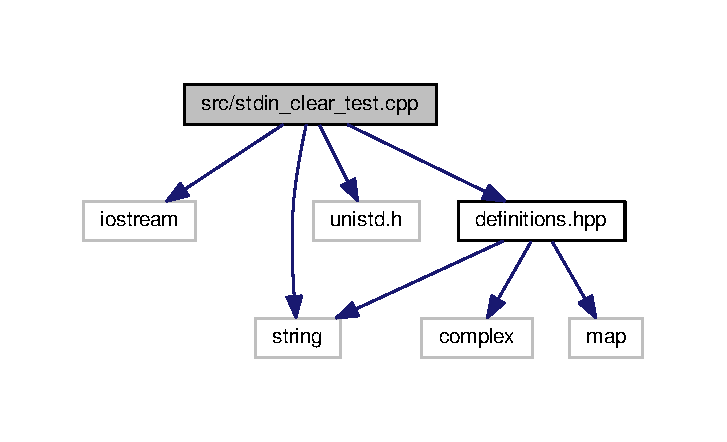
\includegraphics[width=349pt]{stdin__clear__test_8cpp__incl}
\end{center}
\end{figure}
\subsection*{Macros}
\begin{DoxyCompactItemize}
\item 
\#define \hyperlink{stdin__clear__test_8cpp_a698c124f1c293f98840449d6c5b9d984}{C\+O\+U\+N\+T}~80
\end{DoxyCompactItemize}
\subsection*{Functions}
\begin{DoxyCompactItemize}
\item 
int \hyperlink{stdin__clear__test_8cpp_a3c04138a5bfe5d72780bb7e82a18e627}{main} (int argc, char $\ast$$\ast$argv)
\end{DoxyCompactItemize}


\subsection{Detailed Description}
Contains a program to test clearing the stdin buffer. 

\begin{DoxyAuthor}{Author}
Samuel Andrew Wisner, \href{mailto:awisner94@gmail.com}{\tt awisner94@gmail.\+com} 

Nicholas K. Nolan 
\end{DoxyAuthor}


Definition in file \hyperlink{stdin__clear__test_8cpp_source}{stdin\+\_\+clear\+\_\+test.\+cpp}.



\subsection{Macro Definition Documentation}
\hypertarget{stdin__clear__test_8cpp_a698c124f1c293f98840449d6c5b9d984}{\index{stdin\+\_\+clear\+\_\+test.\+cpp@{stdin\+\_\+clear\+\_\+test.\+cpp}!C\+O\+U\+N\+T@{C\+O\+U\+N\+T}}
\index{C\+O\+U\+N\+T@{C\+O\+U\+N\+T}!stdin\+\_\+clear\+\_\+test.\+cpp@{stdin\+\_\+clear\+\_\+test.\+cpp}}
\subsubsection[{C\+O\+U\+N\+T}]{\setlength{\rightskip}{0pt plus 5cm}\#define C\+O\+U\+N\+T~80}}\label{stdin__clear__test_8cpp_a698c124f1c293f98840449d6c5b9d984}


Definition at line \hyperlink{stdin__clear__test_8cpp_source_l00014}{14} of file \hyperlink{stdin__clear__test_8cpp_source}{stdin\+\_\+clear\+\_\+test.\+cpp}.



\subsection{Function Documentation}
\hypertarget{stdin__clear__test_8cpp_a3c04138a5bfe5d72780bb7e82a18e627}{\index{stdin\+\_\+clear\+\_\+test.\+cpp@{stdin\+\_\+clear\+\_\+test.\+cpp}!main@{main}}
\index{main@{main}!stdin\+\_\+clear\+\_\+test.\+cpp@{stdin\+\_\+clear\+\_\+test.\+cpp}}
\subsubsection[{main}]{\setlength{\rightskip}{0pt plus 5cm}int main (
\begin{DoxyParamCaption}
\item[{int}]{argc, }
\item[{char $\ast$$\ast$}]{argv}
\end{DoxyParamCaption}
)}}\label{stdin__clear__test_8cpp_a3c04138a5bfe5d72780bb7e82a18e627}
Tests the ability to clear the stdin buffer. 

Definition at line \hyperlink{stdin__clear__test_8cpp_source_l00022}{22} of file \hyperlink{stdin__clear__test_8cpp_source}{stdin\+\_\+clear\+\_\+test.\+cpp}.


\begin{DoxyCode}
00022                                 \{
00023     \textcolor{keywordtype}{char} text1[\hyperlink{stdin__clear__test_8cpp_a698c124f1c293f98840449d6c5b9d984}{COUNT}];
00024     \textcolor{keywordtype}{char} text2[\hyperlink{stdin__clear__test_8cpp_a698c124f1c293f98840449d6c5b9d984}{COUNT}];
00025 
00026     cout << \textcolor{stringliteral}{"Enter text to ignore: "};
00027     cout.flush();
00028     read(STDIN\_FILENO, &text1, \hyperlink{stdin__clear__test_8cpp_a698c124f1c293f98840449d6c5b9d984}{COUNT});
00029 \textcolor{comment}{//  fflush(stdin);}
00030     cout << endl << \textcolor{stringliteral}{"Enter text to print: "};
00031     cout.flush();
00032     read(STDIN\_FILENO, &text2, \hyperlink{stdin__clear__test_8cpp_a698c124f1c293f98840449d6c5b9d984}{COUNT});
00033     cout << endl << \textcolor{stringliteral}{"In buffer: "} << text2 << endl;
00034 \}
\end{DoxyCode}

\hypertarget{stdin__clear__test_8cpp_source}{\section{stdin\+\_\+clear\+\_\+test.\+cpp}
\label{stdin__clear__test_8cpp_source}\index{src/stdin\+\_\+clear\+\_\+test.\+cpp@{src/stdin\+\_\+clear\+\_\+test.\+cpp}}
}

\begin{DoxyCode}
00001 
00008 \textcolor{preprocessor}{#include <iostream>}
00009 \textcolor{preprocessor}{#include <string>}
00010 \textcolor{preprocessor}{#include <unistd.h>}
00011 
00012 \textcolor{preprocessor}{#include "\hyperlink{definitions_8hpp}{definitions.hpp}"}
00013 
\hypertarget{stdin__clear__test_8cpp_source_l00014}{}\hyperlink{stdin__clear__test_8cpp_a698c124f1c293f98840449d6c5b9d984}{00014} \textcolor{preprocessor}{#define COUNT 80}
00015 
00016 \textcolor{keyword}{using namespace }\hyperlink{namespacestd}{std};
00017 \textcolor{keyword}{using namespace }\hyperlink{namespacevaso}{vaso};
00018 
\hypertarget{stdin__clear__test_8cpp_source_l00022}{}\hyperlink{stdin__clear__test_8cpp_a3c04138a5bfe5d72780bb7e82a18e627}{00022} \textcolor{keywordtype}{int} \hyperlink{stdin__clear__test_8cpp_a3c04138a5bfe5d72780bb7e82a18e627}{main}(\textcolor{keywordtype}{int} argc, \textcolor{keywordtype}{char}** argv) \{
00023     \textcolor{keywordtype}{char} text1[\hyperlink{stdin__clear__test_8cpp_a698c124f1c293f98840449d6c5b9d984}{COUNT}];
00024     \textcolor{keywordtype}{char} text2[\hyperlink{stdin__clear__test_8cpp_a698c124f1c293f98840449d6c5b9d984}{COUNT}];
00025 
00026     cout << \textcolor{stringliteral}{"Enter text to ignore: "};
00027     cout.flush();
00028     read(STDIN\_FILENO, &text1, \hyperlink{stdin__clear__test_8cpp_a698c124f1c293f98840449d6c5b9d984}{COUNT});
00029     fflush(stdin);
00030     cout << endl << \textcolor{stringliteral}{"Enter text to print: "};
00031     cout.flush();
00032     read(STDIN\_FILENO, &text2, \hyperlink{stdin__clear__test_8cpp_a698c124f1c293f98840449d6c5b9d984}{COUNT});
00033     cout << endl << \textcolor{stringliteral}{"In buffer: "} << text2 << endl;
00034 \}
\end{DoxyCode}

%--- End generated contents ---

% Index
\newpage
\phantomsection
\addcontentsline{toc}{chapter}{Index}
\printindex

\end{document}
